%======================================================
% This file is part of
% "AMCOS_booklet"
% Version 1.1 (04/07/2019)
% A LaTeX template for conference books of abstracts
%
% This template is available at:
% https://github.com/maximelucas/AMCOS_booklet
%
% License: GNU General Public License v3.0
%
% Authors:
% Maxime Lucas (ml.maximelucas@gmail.com)
% Pau Clusella
%=======================================================

\documentclass[openany, parskip=full, 12pt, a4]{scrbook}

%======================================================
% This file is part of
% "AMCOS_booklet"
% Version 1.1 (04/07/2019)
% A LaTeX template for conference books of abstracts
%
% This template is available at:
% https://github.com/maximelucas/AMCOS_booklet
%
% License: GNU General Public License v3.0
%
% Authors:
% Maxime Lucas (ml.maximelucas@gmail.com)
% Pau Clusella
%=======================================================

\usepackage[utf8]{inputenc}
\usepackage[T1]{fontenc}
\usepackage{lmodern}

%---------------------------------------------------------
% PACKAGES
%---------------------------------------------------------

% TYPOGRAPHY
\usepackage{xspace}
\usepackage{microtype}
\usepackage{cmbright} % different fonts

% VARIA
\usepackage{color}
\usepackage[table]{xcolor} % loads also »colortbl« %load before tikz if options
\usepackage{scrhack} % fix koma script warning about addtolist
\usepackage{blindtext}
\usepackage{pdfpages} % for cover 
\usepackage{sectsty}

\usepackage{ifthen} % to have online and printed versionw

% GRAPHICS & FIGURES & TABLES
\usepackage{graphicx}
\usepackage{float}
\usepackage{multicol} % for timetable
\usepackage{longtable} % for list of participants over more than 1 page
% \usepackage[top=1.5cm, bottom=1.5cm, right=1.5cm, left=1.5cm]{geometry}
\usepackage[a4paper, margin=2.5cm]{geometry}
\usepackage{setspace}
%\usepackage{wrapfig}
%\usepackage{tikz}
%\tikzset{ar/.style={>=latex, ->}}
%\renewcommand{\arraystretch}{1.2}
%\usepackage[multidot]{grffile}
% \usepackage{booktabs}
\usepackage{caption}

% WANTS TO BE LAST
\usepackage[T1]{fontenc}
\usepackage[utf8]{inputenc}
%\usepackage[ngerman]{babel}
\usepackage[english]{babel}

\renewcommand{\contentsname}{Table of Contents} % Custom table of contents title

\subsectionfont{\large\color{myblue}\underline}  % sets colour of sections



\usepackage[hidelinks]{hyperref}
\hypersetup{pdfpagelayout=TwoPageRight}
% \usepackage[ocgcolorlinks]{hyperref}
% \hypersetup{colorlinks, linkcolor={wolf}, linktocpage=true, citecolor ={tpred}, urlcolor={black}}


%-------------------------------------------------------------
% SETTINGS
%-------------------------------------------------------------
\pagestyle{plain}

\setcounter{secnumdepth}{-2} % remove numbering at any level both for the heading and the toc
%https://tex.stackexchange.com/questions/30122/generate-table-of-contents-when-section-sections-without-numbering-has-been

%-------------------------------------------------------------
% USEFUL DEFINTIONS
%-------------------------------------------------------------

% VARIA 
\newcommand\tab[1][1cm]{\hspace*{#1}}


%======================================================
% This file is part of
% "AMCOS_booklet"
% Version 1.1 (04/07/2019)
% A LaTeX template for conference books of abstracts
%
% This template is available at:
% https://github.com/maximelucas/AMCOS_booklet
%
% License: GNU General Public License v3.0
%
% Authors:
% Maxime Lucas (ml.maximelucas@gmail.com)
% Pau Clusella
%=======================================================

%
% COLORS
%

\definecolor{myorange}{RGB}{255,117,40}
\definecolor{mygray}{RGB}{164, 168, 172}
\definecolor{mywhite}{RGB}{235, 238, 231}
\definecolor{myblue}{RGB}{52, 103, 103}

\newcommand{\primarycolor}{myblue}
\newcommand{\secondarycolor}{mywhite}
\newcommand{\ternarycolor}{mywhite}



\tolerance=1
\emergencystretch=\maxdimen
\hyphenpenalty=10000
\hbadness=10000

%
% BOOKLET VERSIONS
%

% If compilation is done with 'compile.sh', both versions (online and printed) are automatically compiled
% If compilation is done from editor, choose which version to compile below
\makeatletter
\@ifundefined{ifOnline}{% % check if already defined from the command line, if not define \ifOnline
	\expandafter\newif\csname ifOnline\endcsname
	\Onlinefalse %set to \Onlinefalse/\Onlinetrue for printed/online version
}{}
\makeatother

% define \type to input the right version of the abstracts
\ifOnline
\newcommand{\type}{o}
\else
\newcommand{\type}{p}
\fi % end if

%
% ABSTRACT ENVIRONMENTS
%

%----------------------------------------
% online abstract environment
%----------------------------------------
\newenvironment{symposium}[4] %{title}{author}{affiliation}{date}
{\filbreak %avoid page break
	
	{\large \bfseries \textcolor{myblue}{#1}}\newline\vspace{-10pt}\hrule

	{ \bfseries #3}
	\vspace{-10pt}

	{\bfseries \itshape Session chair(s): #2} 
	\vspace{-10pt}

	\textcolor{mygray}{#4}
	
}
{}

\newenvironment{abstract}[4] %{title}{author}{affiliation}{type}
{\filbreak %avoid page break
	
	{\large \bfseries #1}
	
	{\bfseries \itshape #2} 

	{#3}
	
	\textcolor{mygray}{#4}
	
}
{}

\newenvironment{keynote}[4] %{title}{author}{affiliation}{date}
{\filbreak %avoid page break
\begin{flushleft} \setstretch{1.5} 
	
	{\Huge \bfseries \textcolor{myblue}{#1}} 


\setstretch{1} 
\end{flushleft}

	{\large \bfseries \itshape #2}
	\vspace{-10pt}

	\textcolor{mygray}{#4} 

	{ \bfseries #3}\newline\hrule

	
}
{}


\newcommand{\poster}[3] %{title}{author}{affiliation}
{\filbreak %avoid page break
	
	{\bfseries \large #1} \\	
	\tab #2, \textit{#3}
	
}
{}

%----------------------------------------
% tags for talk type (colored circle in abstracts)
%----------------------------------------

\newcommand{\KLtag}{\tikz[baseline={([yshift=-.8ex]current bounding box.center)}]  \node[circle, inner sep=2pt, minimum size=0.5em, color=black, fill=\KLcolor]{\small \bfseries KL};} %colored circle with tag

\newcommand{\IStag}{\tikz[baseline={([yshift=-.8ex]current bounding box.center)}]  \node[circle, inner sep=2pt, minimum size=0.5em, color=black, fill=\IScolor]{\small \bfseries IS};} %colored circle with tag

\newcommand{\CTtag}{\tikz[baseline={([yshift=-.8ex]current bounding box.center)}]  \node[circle, inner sep=2pt, minimum size=0.5em, color=black, fill=\CTcolor]{\small \bfseries CT};} %colored circle with tag

\newcommand{\ITtag}{\tikz[baseline={([yshift=-.8ex]current bounding box.center)}]  \node[circle, inner sep=2pt, minimum size=0.5em, color=black, fill=\ITcolor]{\small \bfseries IT};} %colored circle with tag

%
% PAGE LAYOUT DEFINITIONS
%
\usepackage{etoolbox}

%------------------------------------------------------
% page style: vertical line on the side of each page
%------------------------------------------------------
\usepackage[scale=1,angle=0,opacity=1]{background}
\backgroundsetup{contents={}}

\AddEverypageHook{%
\ifthenelse{%
	\isodd{\thepage} \AND  \thepage>1 % if odd page but not front page
	}{%
	\backgroundsetup{
		color=\secondarycolor,
		position=current page.south east,%
		nodeanchor=south east,
		contents={\rule{10pt}{0.66\paperheight}}
		}
	}{%
	% nothing
	}
%
\ifthenelse{% 
	\NOT \isodd{\thepage} \AND \NOT \thepage=44% if even page
	}{%
	\backgroundsetup{
		color=\secondarycolor,
		position=current page.south west,%
		nodeanchor=south west,
		contents={\rule{10pt}{0.66\paperheight}}
		}
	}{%
	% nothing
	}
\BgMaterial}


%---------------------------------------------------
% chapter heading style
%---------------------------------------------------

\newdimen\mybarpadding
\mybarpadding=1.5em\relax %padding between gcolored bar and chapter name

\RedeclareSectionCommand[%
    ,afterskip=4em plus 1pt minus 1pt%
    ,beforeskip=-1pt%1.2em plus 1pt minus 1pt%
    ,level=0%
    ,toclevel=0%
]{chapter}%

\RedeclareSectionCommand[%
  afterindent=false,
  beforeskip=\baselineskip,
  afterskip=.5\baselineskip
]{section}%

\setkomafont{chapter}{\normalfont\normalsize\bfseries\Huge} % koma-script-specific command

\newcommand*{\mynumberedtest}[1]{% to test whether there is a number
  \if\relax\detokenize{#1}\relax%
  \else%
    #1%
    
  \fi}

%-------------------------------------------------chapter style definition

\renewcommand{\chapterlinesformat}[3]{%
  \Ifthispageodd{%
    \hfill%
    \raisebox{-0.2em}{%
      \makebox[0pt][r]{\textcolor{\primarycolor}{\rule{\paperwidth}{1em}}}%
    }%
    \hspace{\mybarpadding}%
% 	\mynumberedtest{#2}
	\mbox{#3}%
  }{%
%    \hbox{%
%       \mynumberedtest{#2}
      \mbox{#3}%
      \hspace{\mybarpadding}%
      \raisebox{-0.2em}{%
        \makebox[0pt][l]{\textcolor{\primarycolor}{\rule{\paperwidth}{1em}}}%
      }%
%    }%
  }%
}
\makeatother
%---------------------------------------------------------

% TIMETABLE COLORS AND STYLES

% text and backgroud colors
\newcommand{\tbg}{gray} % background
\newcommand{\tfg}{white}
\newcommand{\tbc}{gray!25}

% talk types colors
\newcommand{\IScolor}{myblue!65} % invited speaker
\newcommand{\CTcolor}{white} % contributed talk
\newcommand{\KLcolor}{myorange!45} % keynote lecture
\newcommand{\ITcolor}{yellow!25} %

% row types
\newcommand{\tablebreak}[2]{% {time span}{break name}
	\rowcolor{\tbc} #1 &  \multicolumn{4}{c|}{\bfseries #2} \\ \hline }
\newcommand{\eventtype}[2]{% {time span}{event name}
	#1& \multicolumn{4}{c|}{\cellcolor{\tbg}\color{\tfg}\bfseries #2} \\ \hline }

% column spacing and position
\newcolumntype{L}[1]{%
	>{\raggedright\let\newline\\\arraybackslash\hspace{0pt}}m{#1}}
\newcolumntype{C}[1]{%
	>{\centering\let\newline\\\arraybackslash\hspace{0pt}}m{#1}}
\newcolumntype{R}[1]{%
	>{\raggedleft\let\newline\\\arraybackslash\hspace{0pt}}m{#1}}

%\newcommand{\mytable}{|C{0.15\linewidth}| C{0.05\linewidth}|  C{0.25\linewidth} C{0.1\linewidth} C{0.5\linewidth}|}

\newcommand{\IS}[5]{% {time span}{name}{University}{City, Country}{title}
	#1 &\cellcolor{\IScolor}IS&{\bfseries#2}\newline #4&&#5 \\ \hline}
\newcommand{\CT}[5]{%
	#1 &\cellcolor{\CTcolor}CT&{\bfseries#2}\newline #4&&#5 \\ \hline}
\newcommand{\KL}[5]{%
	#1 &\cellcolor{\KLcolor}KL&{\bfseries#2}\newline #4&&#5 \\ \hline}
\newcommand{\IT}[5]{%
	#1 &\cellcolor{\ITcolor}IT&{\bfseries#2}\newline #4&&#5 \\ \hline}
\newcommand{\tutorial}[5]{%
	#1 && {\bfseries#2}\newline #4 &&#5 \\ \hline}



\usepackage{enumitem}
\setlist[description]{itemsep=-1ex, topsep=0.2pt}

	
\begin{document}


% COVER PAGE
%--------------------------------------------------------------------
% 
\includepdf{pdf_static/cover.pdf}	% our cover was produced with canva.com

	
	
% GENERAL INFORMATION
%---------------------------------------------------------------------
% \vspace*{1cm}
\begin{center}
	\textbf{GENERAL INFORMATION} \\
	\ \\[\baselineskip]

	\textcolor{\primarycolor}{\textbf{Host and Organisers}}	 \\
	Jan Born \\
	\ \\[\baselineskip]
	Max Harkotte \\
	Lisa Bastian \\
	Julia Fechner \\
	\ \\[\baselineskip]
	\vspace*{0.5cm}
	
	\textcolor{\primarycolor}{\textbf {Scientific Committee}}	 \\
	The Psychologie und Gehirn (PuG) 2023 conference is organised in close collaboration with the Fachgruppe Biologische Psychologie und Neuropsychologie of the German Psychological Association (DGPs) and the Deutsche Gesellschaft für Psychophysiologie und ihre Anwendung (DGPA). We thank both speakers, Prof. Hartwigsen (DGPs) and Prof. Hewig (DGPA), for their support in the scientific committee.
	\\[\baselineskip]
	\vspace*{0.5cm}

	\textcolor{\primarycolor}{\textbf {Contact}}	 \\
	\textbf{Website:} https://pug2023.de \\
	\textbf{E-Mail:} organisation@pug2023.de
	\\[\baselineskip]
	\vspace*{0.5cm}

	\textcolor{\primarycolor}{\textbf {Acknowledgementst}}	 \\
	We want to express our thanks to all sponsors for their invaluable financial support. Furthermore, we are grateful for the support of our student assistants in the run-up to the conference and their continuous support during the days of the meeting, ensuring that every question gets answered and every problem gets solved.

	PuG Logo Design by Katja Wahl (kwahl.de)

\end{center}
\mbox{}
\thispagestyle{empty}
\vfill
\begin{center}
	\ \\[20pt] % Please cite us by keeping the following line.
	The open-source \LaTeX{} template, AMCOS\_booklet, used to generate this booklet is available at \url{https://github.com/maximelucas/AMCOS\_booklet}
\end{center}

\newpage


% SPONSORS
%------------------------------------------------------------------
\chapter{Sponsors}
\begin{center}
We thank all our sponsors!
\end{center}

\vfill

\begin{center}
    \begin{tabular}{ c c }
        
\includegraphics[width=0.25\textwidth]{tex/images/sponsors/MES.png} & \hspace*{1cm} \vspace*{0.5cm}
        
\includegraphics[width=0.25\textwidth]{tex/images/sponsors/sr-research.png} \\ 
        
\includegraphics[width=0.25\textwidth]{tex/images/sponsors/Tecan.jpg} & \hspace*{1cm} \vspace*{0.5cm}
        
\includegraphics[width=0.25\textwidth]{tex/images/sponsors/easycap.png} \\ 
        
\includegraphics[width=0.25\textwidth]{tex/images/sponsors/mbt.png} & \hspace*{1cm} \vspace*{0.5cm}
        
\includegraphics[width=0.25\textwidth]{tex/images/sponsors/NIRx.png} \\ 
        \multicolumn{2}{c}{
\includegraphics[width=0.3\textwidth]{tex/images/sponsors/BFA.png}}     
    \end{tabular}
    \end{center}

\vfill

\newpage



% Welcome
%---------------------------------------------------------------------
\chapter{Welcome to Hamburg}
Dear colleagues, or simply put: Moin!
 
It is with great pleasure that we welcome you to the 49th Annual Psychologie und Gehirn (PuG) Conference, which will be held at the Universität Hamburg and the Bürgerhaus Wilhelmsburg from May 29 to June 1, 2024. The PuG is jointly organized with the Fachgruppe Biologische Psychologie und Neuropsychologie (FGBPNP) der Deutschen Gesellschaft für Psychologie  (DGPs) und der Deutschen Gesellschaft für Psychophysiologie und ihre Anwendung (DGPA).
 
We are positively surprised (one might even say overwhelmed) by the huge interest in this year’s PuG conference, and proudly present a program that features a rich set of scientific and networking events, including pre-conference workshops (organized by the Early Career Researchers), 35 scientific symposia with about 150 talks, two poster sessions with over 400 posters, poster flash talks, a Buddy program as well as general assemblies of the organizing societies (DGPs, DGPA) and the Special Interest Group of Open and Reproducible Research (IGOR). Opening and social evenings at the Universität Hamburg and on the historic cargo ship Cap San Diego round off the program. The three keynote lectures given by Karin Roelofs, Katharina von Kriegstein, and Nils Kroemer will certainly be highlights of the conference.
 
We are thrilled to gather an international community of researchers to explore developments and foster collaborations in biological psychology, neuropsychology and adjacent fields. We especially look forward to facilitating meaningful dialogues and collaborations among researchers at all stages of their careers. Hosting this year's conference in Hamburg offers a unique setting known for its dynamic intersection of tradition and innovation. As a city that has long been a gateway to the world, Hamburg mirrors the spirit of discovery and connectivity that we aim to promote in our scientific discussions.
 
Looking forward to welcoming you to Hamburg for an inspiring assembly of minds and ideas!
 
Best regards, the local organizing team of PuG 2024:

Helen Blank, Patrick Bruns, Sebastian Gluth, Tina Lonsdorf, Anja Riesel, Brigitte Röder, Nico Schuck, Lars Schwabe, Jan Wacker

\newpage


% TABLE OF CONTENTS 
%---------------------------------------------------------------------
\tableofcontents


% USEFUL INFO
%------------------------------------------------------------------
\chapter{Useful Information}
% 
\setlength{\parskip}{1em}   

\section*{Conference site plan}

\begin{center}
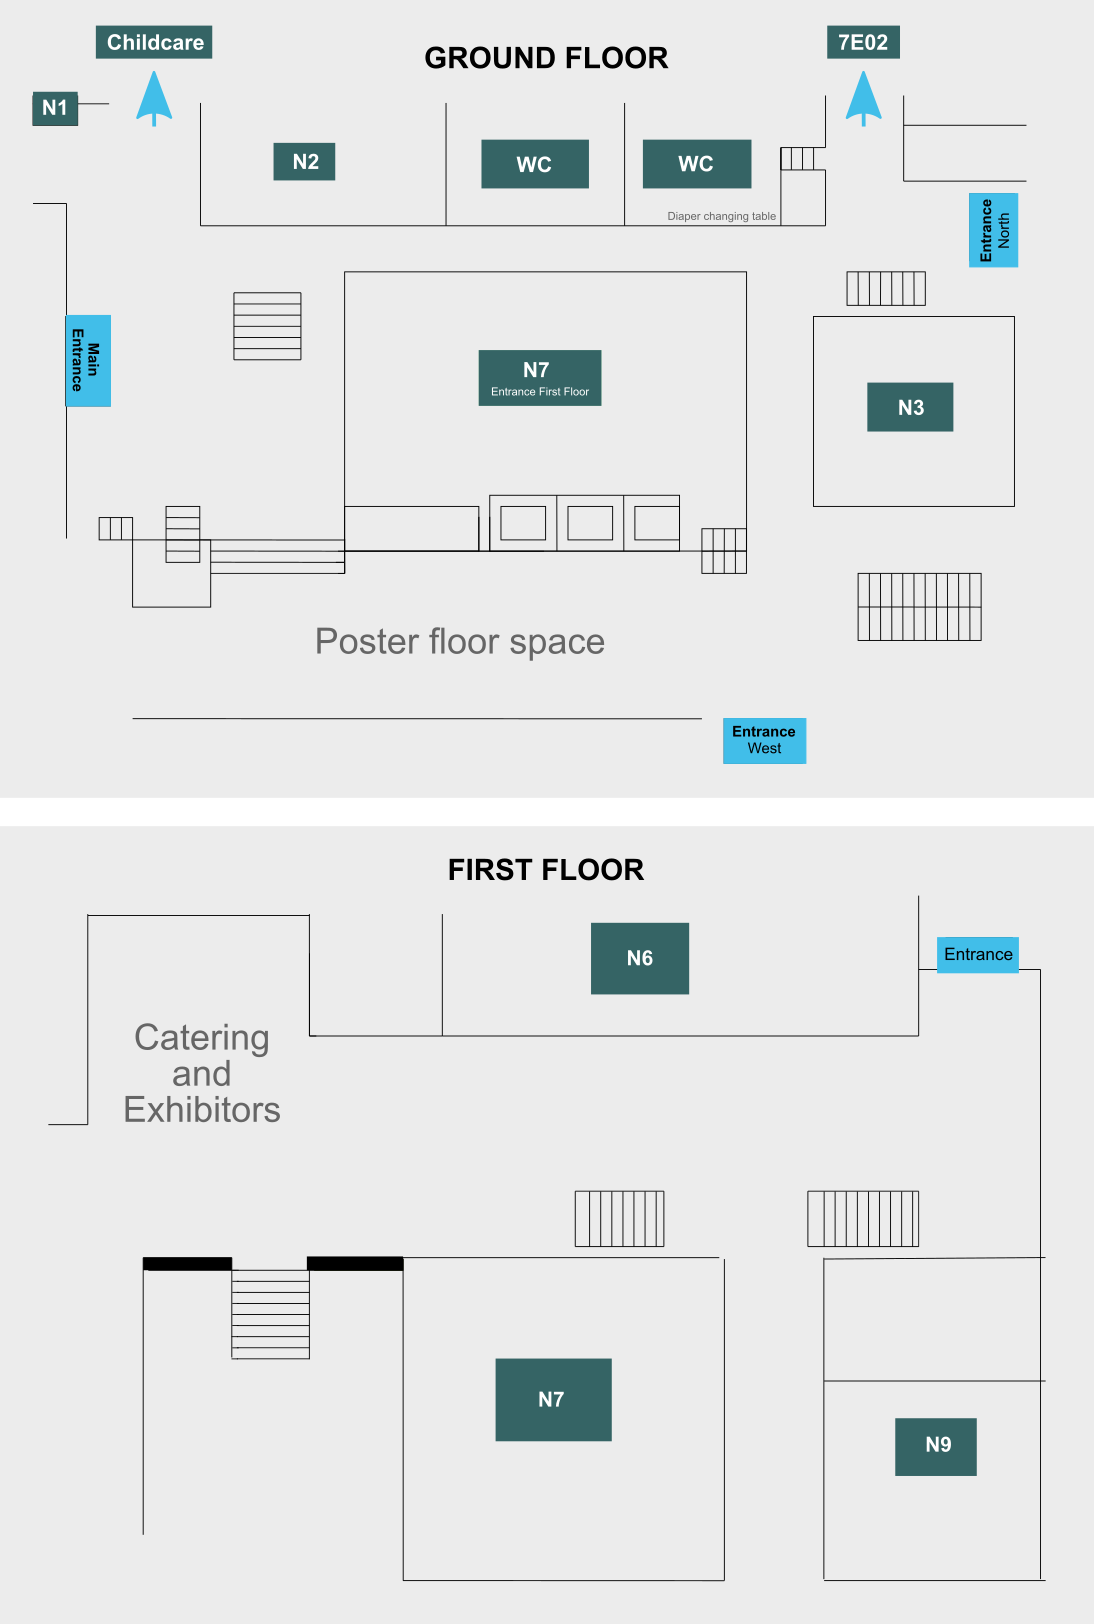
\includegraphics[width=0.8\textwidth]{tex/images/map.png}
\end{center}


\section*{How do I get to the venue?}

In general, we recommend the “Naldo” app, which will show you all the bus times in real time. Additionally, you can find all the bus lines online at https://www.swtue.de/oepnv/fahrplan-und-liniennetz/fahrplaene.html .

The closest bus stop to the venue is called “BG Unfallklinik” and is served by bus lines 5, 13, 14, 17, 18. Central bus stops in the city center are “Hauptbahnhof” (served by all bus lines), “Neckarbrücke” (served by 5, 13, 17, 18) and “Wilhelmstraße” (served by 5, 13, 17, 18).

If you stay in Reutlingen, train MEX 12, MEX 18, IRE 6 and RB 63 will bring you within 10 minutes to the main station in Tübingen. A train departs every half an hour.

\vspace*{-1cm}

\begin{center}
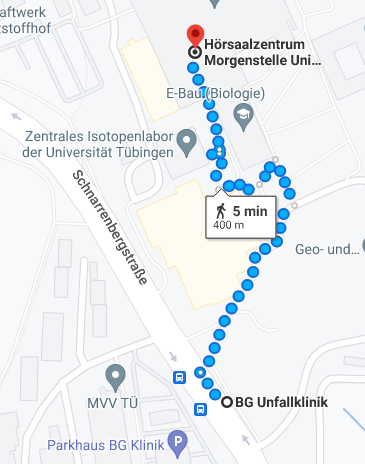
\includegraphics[width=0.5\textwidth]{tex/images/bus.png}
\end{center}

\section*{Accreditation}

Four symposia have been accredited by the Landespsychotherapeutenkammer Baden-Württembergwith with 2 credit points each. If you need a certificate of participation, ask our staff in the respective symposium session: 

\begin{itemize}
\setlength{\itemsep}{-0.8em} 
	\item S04 - Neurobiological Research to Optimize Therapeutic Interventions
	\item S16 - Computational Mechanisms of Learning and Decision-making in Psychiatry
	\item S20 - Prefrontal Cortical Function and Neuromodulation in Mental Disorders
	\item S36 - Deficits in Tactile Perception and their Clinical Implications
\end{itemize}

\section*{Childcare}

We offer childcare in the family room and if the weather is good also outside the conference center. Diaper changing tables can be found on the toilets. If you have any requests don't hesitate to get in touch at the front desk. 

\section*{How do I get to the social evening? And how do I get home later at night?}

The Brauwerk Freistil is located south of the Neckar and easily reachable from the main station or Neckarbrücke within 10 minutes by foot.

\begin{center}
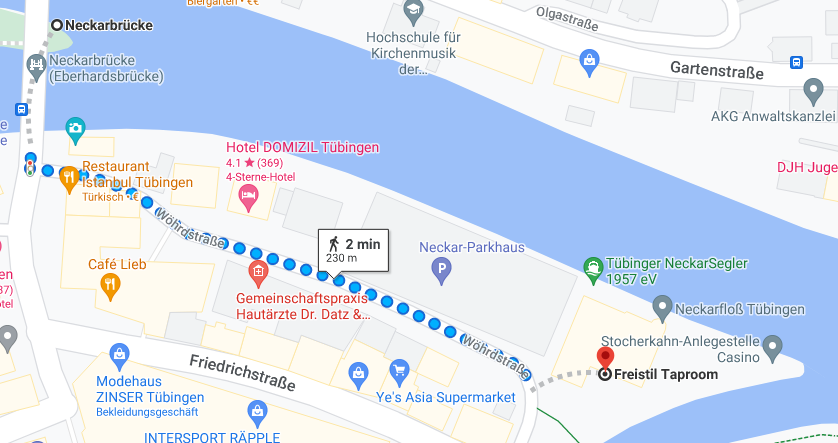
\includegraphics[width=1\textwidth]{tex/images/freistil.png}
\end{center}


Tübingen has a few night busses that run until 3 am. They are marked with an “N”. Alternatively, there are a few taxi companies:

\begin{itemize}
\setlength{\itemsep}{-0.8em} 
	\item Taxi Tübingen 07071 920555 and 0157 80989740
	\item Taxi Akublut 07071 1438591
	\item Taxi Maxi Tübingen 07071 7931064
	\item Taxi Easy 0173 1643229
\end{itemize}


\section*{What is a good place to eat and drink in Tübingen?}

Tübingen has a few nice cafés, restaurants and bars to offer. Coffee places with a nice atmosphere are Café Haag, Café Hanseatica, Willi Tübingen, Suedhang Kaffee and Katesch.
For authentic Swabian food, we recommend Krumme Brücke, Mauganeschtle, Marquardtei, Weinstube Forelle, Ratskeller and Wurstküche. The Neckarmüller is a nice beergarden and the Bären serves Swabian tapas! The Bären and Ratskeller are nice places to stay for one or a few more beers. Other good bars are the Jäger, Stadtpost, Chez Michel and the Irish pub Saints and Scholars.


\section*{And if I need money?}

Contactless payment is available almost everywhere, but some bars still rely on cash. You can find the nearest ATM close to the venue at the BG Klinik at Schnarrenbergstraße.

\begin{center}
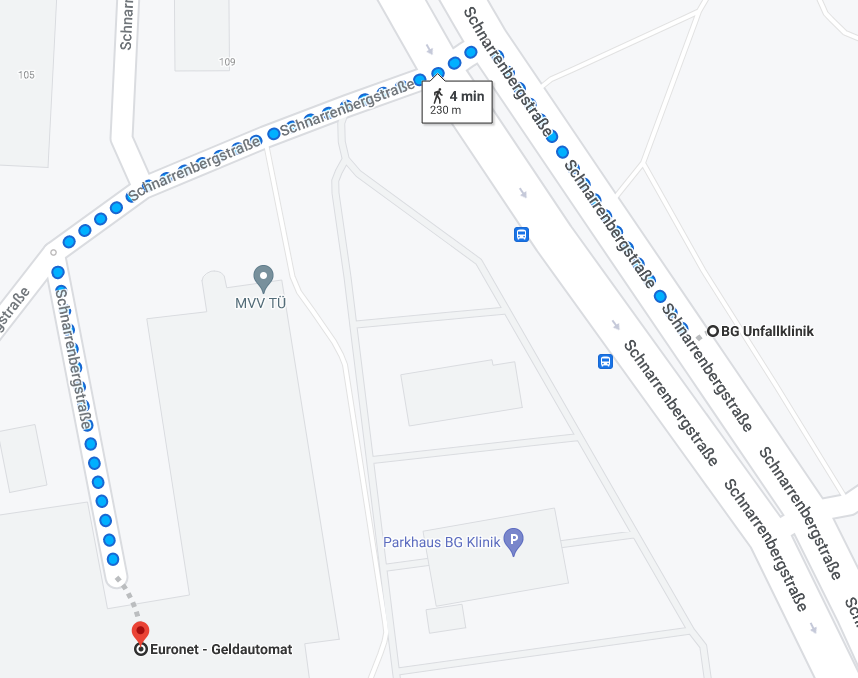
\includegraphics[width=0.8\textwidth]{tex/images/atm.png}
\end{center}


We hope that this information will make your stay as pleasant as possible and that you will enjoy the PuG in Tübingen to the fullest!




% VENUE
%------------------------------------------------------------------
\chapter{Conference Site Plan}
	%Floorplan of the Bürgerhaus Wilhelmsburg
	%\vfill
	\begin{center}
		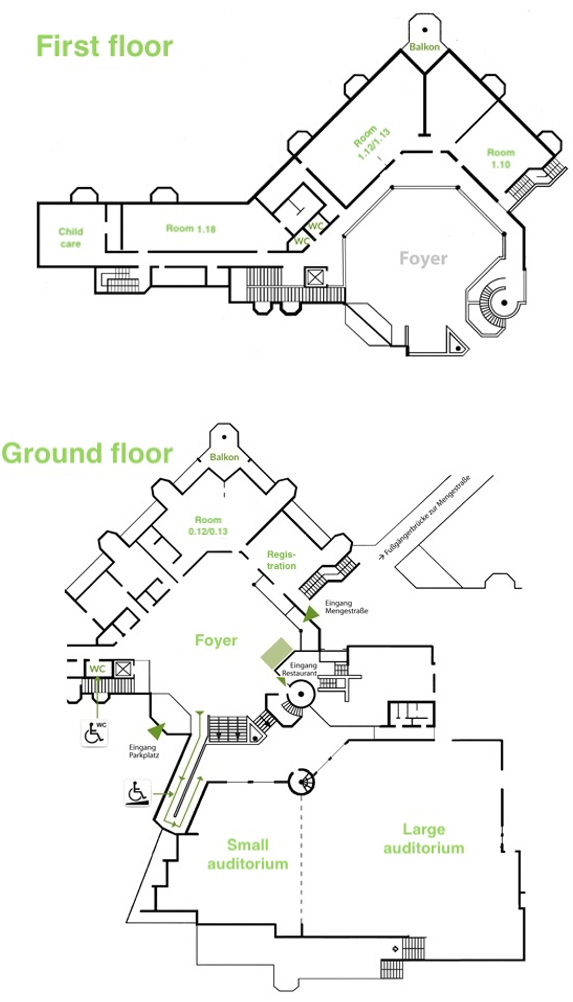
\includegraphics[width=0.8\textwidth]{tex/images/venue/bothfloors.png}
	\end{center}
	
	%\vfill
	
	\newpage


% TIMETABLE 
%---------------------------------------------------------------------
\chapter{Timetable}
% 
\section*{Welcome reception}
We are excited to start the PuG with you on Wednesday, 7th of June, at our welcoming evening! From 6 pm on, you can get your conference documents and register onsite at the front desk at the foyer of the Tagungszentrum Morgenstelle. The evening offers an opportunity for first encounters and to meet your fellow science colleagues. Live music provides a nice ambiance to enjoy free beer, soft drinks and vegetarian/vegan food.

\section*{Social evening}
We look forward to welcoming you to the social evening on Friday at Brauwerk Freistil! The Brauwerk is known for its home-brewed beers, which, unlike its industrial counterparts, make intense flavor experiences instead of simple thirst quenching a priority.

The entrance to the social evening begins directly after the conference program at 6:30 pm. International and local finger food (including vegan options), four free drinks and the beer garden directly at the Neckar are included in the ticket price of 80€. In addition, punting boats, an ice cream and a crepe truck will be provided for a summery ambience in the beer garden. Inside Freistil, you'll find a pool table, dart and shuffle boards, as well as a foosball table to compete against your colleagues. 

From 9:15 pm on there will be live performances by the PuG band and the latin american local band Combo Cumbiale. \textbf{In a short break at around 10 pm, we will award the Poster prizes, the IGOR prize and the prize for the best supervision.} The evening is rounded up by a live set of our DJ. 

Students and PhD students can purchase a party ticket for 35€ for the later part of the evening (entrance from 9:30 pm). Two free drinks are included in the ticket price.

\begin{center}
	
\includegraphics[width=0.3\textwidth]{tex/images/brauwerk.png}
\end{center}

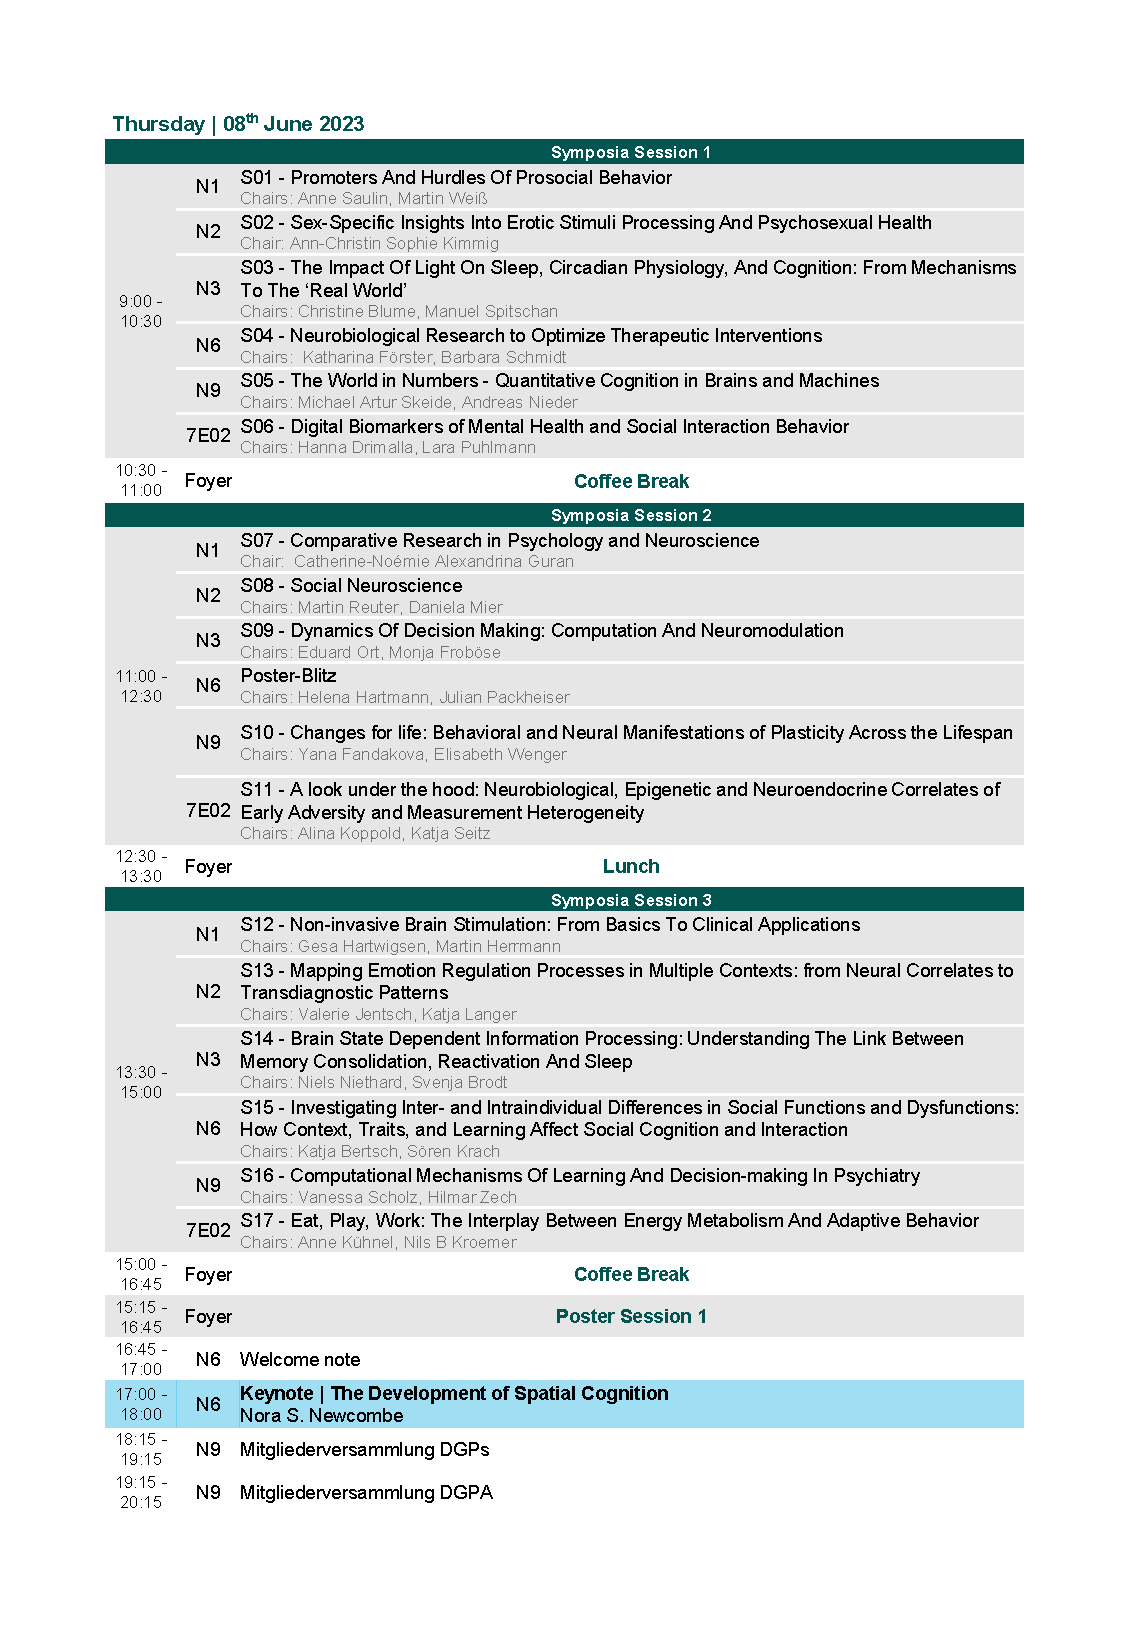
\includepdf[pages=-]{pdf_static/Program.pdf}
\includepdf[scale=0.8]{pdf_static/Social_Event_PuG}


% Definitions of custom environment used here can be found in preamble_booklet.tex file

% The following input commands automatically select the right version 
% (print or online) version of the abstract's .tex
% \type is defined in preamble_booklet.tex and equals:
% 'o' (online) or 'p' (print)


%Thursday
%---------------------------------------------------------------------
\chapter{Thursday | 30. May 2024}
\section{Keynote}

\begin{keynote}
    {Human defensive reactions and their role in approach-avoidance decision making}
    {Karin Roelofs}
    {Thursday 09:15 - 10:15 | ORT}
    {Donders Institute for Brain Cognition and Behavior, Radboud University Nijmegen}

    Behavioural scientists often assume that automatic defensive threat reactions, while essential in explaining animal behavior, only have limited value when it comes to understanding human behavior. There is, however, increasing evidence that defensive reactions, such as freezing, have an impact on subsequent approach-avoidance decisions under acute threat in humans. Understanding the mechanisms that drive such decisions is particularly relevant for patients with anxiety disorders, whose persistent avoidance is key to the maintenance of their anxiety. In recent years, computational psychiatry has made substantial progress formalizing the mechanisms through which we make (mal)adaptive decisions. However, most current models simply ignore the transient psychophysiological state of the decision maker. Here, I argue that the balance between para-sympathetic and sympathetic activity is instrumental in driving the psychophysiological state of freezing, and that it influences approach-avoidance decisions under acute threat in different ways. To illustrate, I first explore the effects of freezing on different kinds of human action decisions under threat. Next, I discuss recent translational (rodent-human) work that has helped to characterize the neural mechanisms implicated in animal and human defensive freezing. Finally, through two prospective longitudinal studies, I show that individual differences in susceptibility to freezing are predictive of the development of anxiety symptoms. 
    Overall, this work suggests that defensive threat reactions and associated psychophysiological states not only affect acute decision making, but also predict long-term symptom development. As such, these factors have great importance for resilience research, and should constitute an integral part of any theory of human decision making.

    % \vspace*{1.0cm}

    \begin{figure}[H]
        \raggedleft
        
\includegraphics[width=0.24\textwidth]{tex/images/keynote_speaker/roeloefs_cropped.png}
    \end{figure}

\end{keynote}


\newpage

\section{Symposia session 1}
\subsection*{Attention and Perception} 
        
                \poster{P.009 - The Influence of Gain and Loss Instruction on Feedback-Processing}
                {A. Kläser}
                {Bergische Universität Wuppertal}
                 
                \poster{P.125 - The interplay of sustained attention and cognitive performance in a Go-NoGo task}
                {L. Stagneth}
                {Universität zu Kiel}
                 
                \poster{P.129 - Interaction of attentional and learning processes during fear acquisition and extinction}
                {E. Tavacioglu}
                {Universität Würzburg }
                 
                \poster{P.151 - The effect of temporal predictability on defensive dynamics during threat anticipation}
                {A. Merscher}
                {Universität Würzburg}
                 
                \poster{P.153 - Neurophysiological Mechanisms of Flexible Integration of Priors in Visual Decisions}
                {G. Iwama}
                {Hertie Institute for Clinical Brain Research, University of Tübingen}
                 
                \poster{P.157 - “Are squirrels as fluffy as they look?” A study of the emergence and relevance of mind wandering in cockpit applications}
                {A. Hamann}
                {Deutsches Zentrum für Luft- und Raumfahrt e.V. DLR}
                 
                \poster{P.193 - Causal inference can explain postdictive multisensory illusions}
                {G. Günaydın}
                {Charité - Universitätzmedizin Berlin}
                 
                \poster{P.197 - Confirmation bias through selective readout of evidence in human cortex}
                {H. Park}
                {Universitätsklinikum Hamburg-Eppendorf}
                 
                \poster{P.231 - Dependence of eye movement-related eardrum oscillations (EMREO) on current sensory input and recent sensory experience}
                {H. Abbasi}
                {Biological Psychology and Neuropsychology, University of Hamburg, Hamburg, Germany}
                 
                \poster{P.311 - Neural correlates of reward-driven attention deployment}
                {T. Feldmann-Wüstefeld}
                {Technische Universität Berlin}
                 
                \poster{P.339 - Causal contributions of prefrontal and intraparietal cortices to audiovisual causal inference}
                {T.  Rohe}
                {Friedrich-Alexander-Universität Erlangen-Nürnberg}
                 
                \poster{P.347 - Variation in neural activity in individuals experiencing minimal and mild-moderate visually induced motion sickness (VIMS)}
                {S.  Berti}
                {Johannes Gutenberg-Universität Mainz}
                 
                \poster{P.389 - Differential effects of self-initiated, externally triggered, and passive movements on action-outcome processing: Insights from EEG and behavior}
                {Y. He}
                {Philipps University Marburg}
                 
                \poster{P.447 - The role of motor representations for working memory when dealing with interference: New evidence by neural oscillations}
                {S.  Ozdemir}
                {Sahcan Ozdemir (Leibniz Research Centre for Working Environment and Human Factors)}
                 
                \poster{P.449 - Resuming after interruptions, to hurry up or to take your time?}
                {S.  Ülkü}
                {Leibniz Research Centre for Working Environment and Human Factors}
                 
                \poster{P.451 - Examining visuomotor expectations in a virtual-reality based hand movement and eye tracking task}
                {F.  Quirmbach}
                {Felix Quirmbach (Technische Universität Dresden)}
                 
                \poster{P.457 - Temporal Prediction in Non-Deterministic Continuous Environments: investigating the role of oscillatory entrainment and interval learning}
                {E.  Hosseini}
                {Max Planck Institute for Biological Cybernetics}
                 
                \poster{P.467 - Effects of reward-based attentional bias modification are unspecific for experimental group and explained by habituation}
                {S.  Kang}
                {Universität Osnabrück}
                 \vspace*{1cm}
        
        \subsection*{Cognition} 
        
                \poster{P.011 - Anticipatory eye movements accompanying prevention and avoidance actions}
                {S. Tonn}
                {Universität Trier}
                 
                \poster{P.017 - Functional segregation of hemispheric asymmetries in EEG across different cognitive domains}
                {P. Reinke}
                {Medical School hamburg }
                 
                \poster{P.049 - Mechanisms of Training-Related Change in Processing Speed: A Drift-Diffusion Model Approach}
                {A. Reinhartz}
                {Medical School Hamburg}
                 
                \poster{P.079 - Individual affective space (Individueller affektiver Raum)}
                {F. Horn}
                {Universität Regensburg}
                 
                \poster{P.099 - Exercise-induced Effects on Neural Correlates of Cognition and Emotion Regulation}
                {L. Wallenwein}
                {Universität Konstanz}
                 
                \poster{P.105 - Implicit and explicit emotion regulation and response inhibition in adult ADHD}
                {A. Sebastian}
                {Universitätsklinikum Mainz}
                 
                \poster{P.113 - Motivational Context and Error Processing in Impulsivity and Compulsivity}
                {R. Overmeyer}
                {TU Dresden }
                 
                \poster{P.143 - Effects of Cortisol on Path Integration}
                {O. Akan}
                {Osman Akan}
                 
                \poster{P.159 - Exploring the Influence of Catecholaminergic Modulation on Event Segmentation: Insights from Pharmacological Manipulation}
                {A. Prochnow}
                {Universitätsklinikum Dresden}
                 
                \poster{P.161 - Modulation of Neural Correlates of Model-based Performance with Impulsivity and Compulsivity}
                {K. Dück}
                {TU Dresden}
                 
                \poster{P.183 - Heuristic pruning of the decision tree at low probabilities and probability discounting in three-step planning in young and older adults}
                {S. Sass}
                {TU Dresden}
                 
                \poster{P.189 - Reward morphs non-spatial cognitive maps in humans}
                {N. Moneta}
                {Universität Hamburg}
                 
                \poster{P.199 - Memory effects of visual and olfactory landmark information in human wayfinding}
                {M. Schwarz}
                {Justus Liebig Universität Gießen}
                 
                \poster{P.205 - Mid-Frontal Brain Signal Variability Predicts Auditory Discrimination Performance}
                {N. Kloosterman}
                {Universität zu Lübeck}
                 
                \poster{P.207 - Does affective self-other distinction require cognitive resources?}
                {K. Döhr}
                {Universität zu Lübeck}
                 
                \poster{P.219 - Neural phase reset as a mechanism of predicting time across different sensory modalities}
                {R. Burke}
                {Rebecca Burke}
                 
                \poster{P.229 - Is rest simply the best? An Investigation of the effectiveness and acceptance of a rest break and a motor task regarding the reduction of Mental Fatigue}
                {V. Rubahn}
                {Deutsches Zentrum für Luft- und Raumfahrt e.V. (DLR)}
                 
                \poster{P.235 - Alterations of Functional Network Topology Underlying Cognitive Flexibility and Stability in Schizophrenia}
                {A. Zahedi}
                {University of Muenster}
                 
                \poster{P.237 - Anyplace, Anywhere, Anytime- Investigating the Pe and its Narcissism-Related Variations Using Cluster-Based Permutation Testing}
                {M. Kückelhaus}
                {Maya Kückelhaus}
                 
                \poster{P.242 - The cerebellum is involved in processing reward prediction errors - evidence from patients with cerebellar stroke}
                {D. Huvermann}
                {Heinrich-Heine-Universität Düsseldorf}
                 
                \poster{P.265 - FEEDBACK MONITORING DURING ACTIVE AND OBSERVATIONAL LEARNING IN OBSESSIVE-COMPULSIVE DISORDER: AN ERP STUDY}
                {J. Vahedi}
                {Julian Vahedi}
                 
                \poster{P.269 - The influence of cardiorespiratory phase locking on voluntary action initiation and sense of agency: preliminary results}
                {M. Gerosa}
                {Max Planck Institute for Human Cognitive and Brain Sciences}
                 
                \poster{P.271 - Negative anticipation leads to a preference for experiencing intense pain earlier rather than later in time}
                {M. Habermann}
                {Universität Hamburg}
                 
                \poster{P.277 - Prediction of individual cognitive test performance based on imaging and non-imaging data in older adults}
                {C. Krämer}
                {Camilla Krämer}
                 
                \poster{P.291 - Is task similarity of functional connectivity across tasks related to modality-specific dual-task interferences?}
                {M. Mückstein}
                {Marie Mückstein}
                 
                \poster{P.297 - It’s about time: Specific and unspecific effects of future simulation on farsighted decisions}
                {H. Schultz}
                {TU Dresden}
                 
                \poster{P.305 - Beyond Expectation: A Novel Paradigm Disentangling Semantic Processing and Predictive Coding}
                {A. Petukhova}
                {Philipps-Universität Marburg}
                 
                \poster{P.319 - The functional form of context-dependence in perceptual multialternative decisions}
                {M.  Tohidimoghaddam}
                {Department of Neurophysiology and Pathophysiology, University Medical Center Hamburg-Eppendorf, Hamburg, Germany}
                 
                \poster{P.325 - An inductive bias for slow features in human reinforcement learning}
                {N. Hedrich}
                {Universität Hamburg}
                 
                \poster{P.327 - Dopamine's role in visual imagery: Pilot data from an experimental pharmacological study}
                {J. Karneboge}
                {Universität Bonn}
                 
                \poster{P.375 - Walk-n-talk: Gait patterns and verbal communication under changing environmental conditions}
                {J.  Herrmann}
                {Universität Lübeck}
                 
                \poster{P.385 - Pupil dilation offers a time-window on prediction error}
                {O. Colizoli}
                {Radboud University}
                 
                \poster{P.395 - Neural dynamics of predicting others' decisions}
                {E. Stuchlý}
                {Erik Stuchlý (University of Hamburg)}
                 
                \poster{P.409 - Prefrontal Cortex and Hippocampus Jointly Guide Flexible Working Memory}
                {M.  Fernandez}
                {Mariana Lomeli Fernandez}
                 
                \poster{P.431 - Tracking Representational Dynamics across Brain States during Actions}
                {P. Wendiggensen}
                {TU Dresden}
                 
                \poster{P.439 - Context-Dependent Choice Biases in Human Reinforcement Learning}
                {B.  Wagner}
                {Ben Jonathan Wagner (Technische Universität Dresden, Professur für Kognitive Computationale Neurowissenschaft)}
                 
                \poster{P.459 - On the trail of the Hot Hand effect in 500 million online card games}
                {M. Guggenmos}
                {Health and Medical University Potsdam}
                 
                \poster{P.461 - Hierarchical representations in flexible planning}
                {R. Bayramova}
                {Rena Bayramova (Max Planck Institute for Human Cognitive and Brain Sciences)}
                 
                \poster{P.471 - The Differential Impact of Gaze Direction and Mouth Expressions on Social Inclusion Perception}
                {Y. Yang}
                {Freie Universität Berlin}
                 \vspace*{1cm}
        
        \subsection*{Brain and Periphery, Neuroendocrinology, and Stress} 
        
                \poster{P.015 - Post-retrieval stress impairs subsequent memory depending on hippocampal memory trace reinstatement during reactivation}
                {H. Heinbockel}
                {Universität Hamburg}
                 
                \poster{P.029 - OpenTSST – An open web platform for large-scale, video-based motion analysis during acute psychosocial stress}
                {M. Kurz}
                {Friedrich-Alexander-Universität Erlangen-Nürnberg}
                 
                \poster{P.089 - Sex-specific associations between acute cortisol and neural stress responses:  The Regensburg Burnout Project}
                {G. Henze}
                {Charité Universitätsmedizin Berlin}
                 
                \poster{P.103 - Mapping the Brain's Stress Response: Network Interactions in Functional Cortical Gradients}
                {A. Patyczek}
                {Max-Planck-Institut für Kognitions- und Neurowissenschaften}
                 
                \poster{P.117 - Effects of emotion regulation on repeated exposure to stress}
                {K. Langer}
                {Ruhr-Universität Bochum}
                 
                \poster{P.121 - Salivary testosterone predicts self-dislike in women with borderline personality disorder}
                {E. Kulakova}
                {Charité Universitätsmedizin Berlin}
                 
                \poster{P.133 - Non-genomic and genomic cortisol effects on the return of fear after contextual extinction generalization}
                {J. Caviola}
                {Ruhr-Universität Bochum}
                 
                \poster{P.137 - Determining the direction of the relationship between burnout symptoms and social support: A cross-lagged panel analysis}
                {M. Wekenborg}
                {TU Dresden}
                 
                \poster{P.141 - Neural correlates associated with cortisol effects on face recognition}
                {L. Poetzl}
                {Ruhr-Universität Bochum}
                 
                \poster{P.145 - Creating strong and context-independent extinction memories with physical exercise vs. psychosocial stress}
                {L. Wolsink}
                {Ruhr-Universität Bochum}
                 
                \poster{P.169 - (f)MRI-based variables as predictors for the identification of cortisol stress response trajectories}
                {R. Lipka}
                {Charité - Universitätsmedizin Berlin}
                 
                \poster{P.191 - Empathic stress in the mother-child dyad: Multimodal evidence for empathic stress in children observing their mothers during direct stress exposure}
                {J. Blasberg}
                {Universitätsklinikum Jena}
                 
                \poster{P.247 - Human vs. AI: The Impact of Simulated Medical Consultations on Individual Subjective Stress and Salivary Cortisol Levels}
                {C. Mayer}
                {Universität Heidelberg}
                 
                \poster{P.273 - Investigation into the relationship between long-term cortisol output and acute stress reactivity}
                {S. Vogel}
                {Medical School Hamburg}
                 
                \poster{P.299 - The influence of glucose on the neural, cardiovascular and endocrine response to stress - an experimental study with near-infrared spectroscopy (fNIRS)}
                {M. Meier}
                {Universität Konstanz, UPK Basel}
                 
                \poster{P.337 - Oscillatory Brain Activity Related to Evoked Phantom Limb Pain}
                {A.  Serian}
                {Zentralinstitut für Seelische Gesundheit Mannheim}
                 
                \poster{P.355 - Habituation of the biological response to repeated psychosocial stress: a systematic review and meta-analysis}
                {M.  Barthel}
                {Medical School Hamburg}
                 
                \poster{P.359 - Stress associated epigenetic changes in saliva (STEPS): a conceptual replication pilot study.}
                {N. Reinsberg}
                {Medical School Hamburg}
                 
                \poster{P.369 - Examining the impact of open-label-placebos on anxiety, stress and cortisol concentration in the context of a real-life stressor}
                {C.  Liedtke}
                {Medical School Berlin}
                 
                \poster{P.387 - The relevance of individual differences in coping styles for cortisol stress reactivity and habituation during repeated psychosocial stress}
                {S.  Illius}
                {Sabrina Illius}
                 
                \poster{P.397 - The Gut Microbiome: A Common Factor in Obesity and Depression}
                {L.  Kubin}
                {Luca Celina Kubin}
                 
                \poster{P.399 - The Romantic Partner’s Chemosensory Presence Increases Psychological and Autonomic Stress Responses}
                {F.  Spengler}
                {Universität Freiburg}
                 
                \poster{P.405 - Unraveling the neuronal mechanisms of Exercise-Induced Hypoalgesia: Insights from High-Intensity Interval Training}
                {M.  Geisler}
                {Universität Jena}
                 
                \poster{P.443 - Study Protocol: Maternal Prenatal Distress, Infant Difficult Temperament and Cortisol as Prenatal Mediator, a Systematic Review and Meta-Analysis}
                {F. Sörensen}
                {Ferdinand Sörensen (Universitätsklinikum Tübingen)}
                 \vspace*{1cm}
        
        \subsection*{Affective Neuroscience} 
        
                \poster{P.031 - Examining the Relationship Between Heart Rate Variability and Frontal Alpha Asymmetry: Do Heart and Brain Align?}
                {A. Sahm}
                {Universität Konstanz}
                 
                \poster{P.081 - Influence of interstimulus variability on processing of selectively attended emotional facial expressions}
                {J. Schmuck}
                {Universität Bonn}
                 
                \poster{P.085 - ERP effects of SOA-modulated spatial pre-cueing of emotional distractors}
                {V. Shivani}
                {Universität Bonn }
                 
                \poster{P.095 - The Impact of Aversive Contexts on Visuocortical and Physiological Correlates of Defensive Behavior During Threat Generalization}
                {Y. Stegmann}
                {Universität Würzburg}
                 
                \poster{P.111 - How do people react to and learn from emotional social encounters? A multimodal social conditioning study in immersive virtual reality}
                {S. Gado}
                {Universittät Würzburg }
                 
                \poster{P.123 - EEG microstates in social and affective neuroscience}
                {B. Schiller}
                {Universität Freiburg}
                 
                \poster{P.131 - Impact of restrictive eating/dieting on coding of subjective preferences for edible and non-edible rewards in the event-related potential (ERP)}
                {C. Assen}
                {Medical School Hamburg}
                 
                \poster{P.149 - Psychosexual health during the menopause transition}
                {F. Weinmar}
                {Universität Tübingen}
                 
                \poster{P.167 - No cardiac phase bias for threat perception under naturalistic conditions in immersive virtual reality}
                {M. Gaebler}
                {Max-Planck-Institut für Kognitions- und Neurowissenschaften Leipzig}
                 
                \poster{P.175 - Deciphering the Impact of a Trauma-Analogue: Assessing Individual Vulnerability through Heart Rate, Cognitive Control, and Memory Reactivation}
                {L. Petersdotter}
                {Lund University}
                 
                \poster{P.195 - I freeze, therefore I act:  Disentangling freezing responses linked to threat  versus action preparation}
                {J. Teigeler}
                {Universität Würzburg}
                 
                \poster{P.217 - Comparing behavioural responses and activation patterns of thermal heat and cuff pressure pain – an explorative fMRI study}
                {J. Nold}
                {Universität Hamburg}
                 
                \poster{P.225 - Mechanisms of Motivated Endogenous Pain Modulation}
                {L. Asan}
                {University Medical Center Hamburg-Eppendorf}
                 
                \poster{P.295 - An experimental and computational test of links between self-esteem, control experience, and positive affect}
                {J. Weis}
                {Jan Weis}
                 
                \poster{P.301 - The evaluation of presumed deepfakes with different basic emotional expressions depends on valence}
                {J. Baum}
                {Humboldt-Universität zu Berlin}
                 
                \poster{P.353 - Pre-stimulus oscillatory activity modulates emotional facial expression processing}
                {C. Jaap}
                {Carina Jaap (Universitätsklinikum Eppendorf; Systemische Neurowissenschaften)}
                 
                \poster{P.361 - Real-time continuous rating of affective experience in immersive Virtual Reality.}
                {a. fourcade}
                {Max Planck Institute for Human Cognitive and Brain Sciences}
                 
                \poster{P.363 - Deciphering Empathy:  Neural Insights into Cognitive and Affective Empathy and Personal Distress}
                {A.  Wolber}
                {Alexander Wolber}
                 
                \poster{P.393 - An Overestimation of Safety? The Impact of Acoustic Startle Probes on Task Effects in a Threat of Shock Paradigm}
                {H. Carsten}
                {Hannes Per Carsten (Institute of Psychology)}
                 
                \poster{P.435 - Exploring anhedonia in dopaminergic antidepressant mood effects}
                {L.  Chuang}
                {Philipps-Universität Marburg}
                 \vspace*{1cm}
        
        \subsection*{Individual Differences and (Epi)Genetics} 
        
                \poster{P.047 - Gene-Environment Interaction Effects on Perceived Stress and the Cortisol Awakening Response in Daily Life over 13 Months}
                {S. Wüst}
                {Universität Regensburg}
                 
                \poster{P.087 - Can Personality Traits be Predicted from Resting-state EEG Oscillations? A Replication Study}
                {C. Frühlinger}
                {Universität Hamburg}
                 
                \poster{P.201 - Testing the mismatch-hypothesis for chronic pain – Integrating insights from ancient, comparative and neuroimaging genomics}
                {O. Goltermann}
                {Universität Hamburg}
                 
                \poster{P.203 - Come closer if your dare: A validation of the revised Reinforcement Sensitivity Theory by behavioral responses to positive and negative stimuli}
                {S. Hogeterp}
                {Universität Bonn}
                 
                \poster{P.211 - Enhancing Achievement Motivation: Neurocognitive Insights into Task Difficulty Selection}
                {Y. Wilk}
                {Universität zu Köln}
                 
                \poster{P.251 - Continuous glucose monitoring across the menstrual cycle: Associations between glucose levels, mood and sex hormones}
                {M. Grahlow}
                {Universitätsklinikum Tübingen}
                 
                \poster{P.303 - Cognitive motivation influences effort discounting in the presence of real but not sham or no feedback}
                {J. Zerna}
                {Josephine Zerna}
                 
                \poster{P.441 - Epigenetic signatures of childhood maltreatment in a high-risk sample - a replication study}
                {E. Unternaehrer}
                {Eva Unternaehrer (UPK Basel, Schweiz)}
                 
                \poster{P.463 - Phenome-wide association study of pain- and anxiety-linked endocannabinoid gene variation FAAH C385A}
                {A. Gärtner}
                {TU Dresden}
                 \vspace*{1cm}
        
        \subsection*{Social and Environmental Neuroscience} 
        
                \poster{P.075 - cooperative and competitive interactions in a social foraging task.}
                {S. Khoneiveh}
                {Universitätsklinikum Hamburg-Eppendorf UKE}
                 
                \poster{P.147 - The Impact of Attachment on Stress Resonance in Romantic Partnerships}
                {M. Gallistl}
                {Universität Leipzig}
                 
                \poster{P.171 - Temporal presence in computer-mediated social encounters modulates neural but not behavioral and electrodermal indices of empathy for pain}
                {J. Heimann}
                {Universität zu Lübeck}
                 
                \poster{P.213 - Effect of social presence on approach-avoidance conflicts – Preliminary data from a 7T fMRI experiment}
                {J. Bischofberger}
                {Universitätsklinikum Würzburg}
                 
                \poster{P.275 - The (in)stability of incentivized prosocial behavior}
                {A. Saulin}
                {Universitätsklinikum Würzburg}
                 
                \poster{P.349 - White matter differences in monozygotic twins discordant for obsessive-compulsive disorder}
                {P. Keutz}
                {Patricia Keutz}
                 \vspace*{1cm}
        
        \subsection*{Development and Aging} 
        
                \poster{P.077 - Personality Traits and Cognitive Reserve – High Openness Benefits Cognition in the Presence of Age-related Brain Changes}
                {A. Coors}
                {Columbia University Medical Center}
                 
                \poster{P.083 - The development of receptive fields for numerosity perception in the human brain}
                {G. Jeong}
                {Max-Planck-Institut für Kognitions- und Neurowissenschaften Leipzig}
                 
                \poster{P.119 - Curiosity and surprise differentially affect long term memory across the adult lifespan}
                {N. Bunzeck}
                {Universität zu Lübeck }
                 
                \poster{P.177 - Central insulin effects on appetitive decision-making in older adults}
                {C. Moreno}
                {Universitätsklinikum Hamburg-Eppendorf}
                 
                \poster{P.239 - How do childhood negative life events and brain development relate to depression in young adulthood?}
                {N. Vetter}
                {Universität zu Köln}
                 
                \poster{P.263 - Developmental changes in theta band activity during continuous sensorimotor integration: an EEG study}
                {A. Böttcher}
                {TU Dresden}
                 
                \poster{P.309 - Self-Esteem Dynamics and Reactivity towards Social Feedback in Adolescents with and without Symptoms of Borderline Personality Disorder}
                {K. Gregorova}
                {Uniklinikum Würzburg}
                 
                \poster{P.315 - Healthy aging increases the lexical bias in speech perception independent of individual hearing acuity}
                {N. Pfitzner}
                {Nele Lea Pfitzner}
                 
                \poster{P.323 - The Impact of Smoking Initiation in Late Adolescence on Functional Network Organization in the Transition to Early Adulthood}
                {D. Fiesel}
                {Christian-Albrechts-Universität zu Kiel}
                 
                \poster{P.329 - Real-time fMRI neurofeedback reduces hippocampal hyperactivity and improves pattern separation in Mild Cognitive Impairment}
                {K. Klink}
                {Katharina Klink}
                 
                \poster{P.343 - Dense-sampling fMRI to test the expansion and renormalization of BOLD responses caused by learning interventions}
                {A.  Enge}
                {Alexander Enge (Max Planck Institute for Human Cognitive and Brain Sciences)}
                 
                \poster{P.379 - Blocked learning curriculum reduces age-related deficits in memory}
                {X.  Ren}
                {Xiangjuan Ren}
                 
                \poster{P.381 - Examining the influence of efficacy and reward on cognitive control across development}
                {S.  Kleber}
                {Zentrum für Psychische Gesundheit, Klinik und Poliklinik für Kinder-und Jugendpsychiatrie, Psychosomatik  und Psychotherapie des Uniklinikum Würzburg}
                 
                \poster{P.407 - Individual Differences in Resting-State EEG Markers of Dementia and Normal Aging}
                {O.  Labrenz}
                {Oliver Labrenz (Brandenburg Medical School)}
                 
                \poster{P.429 - False Recognition in Aging is Due To an Emphasis on Semantic Information at Encoding}
                {L.  Naspi}
                {Loris Naspi (Humboldt Univerity of Berlin)}
                 
                \poster{P.437 - Cognitive and Motor Adaptation Across the Lifespan}
                {J.  Falck}
                {Goethe-Universität Frankfurt am Main}
                 \vspace*{1cm}
        
        \subsection*{Disorders and Interventions} 
        
                \poster{P.091 - Sugar Rush to Remember: Sweetening the Fear Memory Circuit with Glucose}
                {M. Lehnert}
                {Universität des Saarlandes}
                 
                \poster{P.163 - Improving Executive Functions: Assessing the Impact of a Three-Week At-Home Cognitive Training on Mediofrontal Negativities in OCD Patients}
                {M. Ganser}
                {Medical School Berlin}
                 
                \poster{P.165 - Neural correlates of cognitive control in problematic internet use}
                {C. Turhan}
                {MSB Medical School Berlin}
                 
                \poster{P.181 - Ruminative emotion regulation is associated with increased fronto-limbic activity, but decreased fronto-limbic connectivity in young patients with depression}
                {K. Förster}
                {TU Dresden}
                 
                \poster{P.187 - From Cyberspace to the Laboratory to Clinical Context: Validation of a digital, pre-recorded exposure intervention for public speaking anxiety – a study protocol}
                {S. Klein}
                {Universität des Saarlandes}
                 
                \poster{P.209 - A neural signature of touch aversion and interoception in Borderline Personality Disorder}
                {J. Voelter}
                {Carl-von-Ossietzky Universität Oldenburg}
                 
                \poster{P.223 - Increasing the smoking cessation success rate by enhancing improvement of self-control through sleep-amplified memory consolidation}
                {M. Kroth}
                {Zentralinstitut für Seelische Gesundheit Mannheim}
                 
                \poster{P.249 - Electrophysiological Correlates of Vulnerability and Resilience to Helplessness}
                {A. Forster}
                {Universität Würzburg}
                 
                \poster{P.259 - Breathing Apperception Training: Evaluation of a breath-centered intervention program to influence psychological and biological mechanisms of depression and anxiety}
                {Ç. Gürsoy}
                {Zentralinstitut für Seelische Gesundheit, Mannheim}
                 
                \poster{P.287 - The tell-tale heart: Resting heart rate predicts emotional interference in a transdiagnostic outpatient sample}
                {S. Tholl}
                {University of Konstanz}
                 
                \poster{P.313 - Differences in the reassessment of choices in an unstable environment in twins discordant for obsessive–compulsive disorder}
                {A. Seidel}
                {Medical School Hamburg}
                 
                \poster{P.345 - Cognitive control and error processing in OCD—behavioral and electrophysiological markers in discordant monozygotic twins}
                {A.  Schönbohm}
                {Annika Schönbohm}
                 
                \poster{P.351 - Voxel-wise intrinsic measures in sensorimotor cortices characterises substance use disorders: An ALE meta-analysis}
                {M.  Fascher}
                {Medical School Hamburg}
                 
                \poster{P.365 - Walking the Black Dog: A Systematic Review and Meta-Analysis of Walking as an Intervention in the context of Depression}
                {L.  Rupp}
                {Lydia Helen Rupp}
                 
                \poster{P.367 - How Well Can We Explain Paranoia? A Machine Learning Approach to Aetiological Models of Persecutory Delusions}
                {S. Denecke}
                {Saskia Denecke}
                 
                \poster{P.411 - Altered functional connectivity in spider phobia normalised after one-session treatment}
                {M.  Muehlhan}
                {Medical School Hamburg}
                 
                \poster{P.415 - Exposure to relaxation-associated odors during sleep reduces sleep spindles in people with frequent nightmares}
                {C. Sayk}
                {Clara Sayk (Universität zu Lübeck, Translational Psychiatry Unit)}
                 
                \poster{P.445 - Computational Modeling of Belief Updating across Social versus Non-Social Contexts in Individuals with High versus Low Paranoia}
                {A.  Bott}
                {Antonia Bott (Clinical Psychology and Psychotherapy, Universität Hamburg)}
                 \vspace*{1cm}
        
        \subsection*{Computational Methods and Neuroimaging} 
        
                \poster{P.101 - A Graphical User Interface for Game-Theoretic Lesion-Symptom Mapping}
                {S. Dixit}
                {Universitätsklinikum Hamburg-Eppendorf}
                 
                \poster{P.109 - Past and future episodic cues modulate temporal discounting via multiple common computational routes.}
                {K. Knauth}
                {Universität zu Köln}
                 
                \poster{P.115 - Structural-Functional Brain Network Coupling During Task Performance Reveals Intelligence-Relevant Communication Strategies}
                {J. Popp}
                {Universität Würzburg}
                 
                \poster{P.127 - Communication with Surprise – Computational and Neural Mechanisms for Non-Verbal Human Interactions}
                {T. Buidze}
                {Universitätsklinikum Hamburg-Eppendorf}
                 
                \poster{P.155 - Exploring False Memories through Neural Network Word Embeddings}
                {S. Sander}
                {Zentralinstitut für Seelische Gesundheit Mannheim}
                 
                \poster{P.215 - Neural substrates underlying overriding automatic behavioral tendencies in approach-avoidance conflict decisions}
                {M. Chen}
                {Universität Würzburg}
                 
                \poster{P.241 - Well, would you look at the time - Comparing of the influence of different cortical organizational schemes on the temporal layout of the cortex}
                {F. Mecklenbrauck}
                {Universität Münster}
                 
                \poster{P.257 - Neural correlates of individual stress responses and problematic alcohol use}
                {L. Wazulin}
                {Zentralinstitut für Seelische Gesundheit Mannheim}
                 
                \poster{P.279 - Tyrosine reduces discounting of delayed rewards using a Bayesian DDM framework in a mixed-gender sample}
                {C. Nientimp}
                {Universität zu Köln}
                 
                \poster{P.289 - Performance and exploration strategies in recurrent neural networks during reinforcement learning depend on network capacity.}
                {H. Flimm}
                {Department of Psychology, Biological Psychology, University of Cologne}
                 
                \poster{P.321 - Glutamatergic and GABAergic modulation of cortical temporal dynamics}
                {A. Dias Maile}
                {Heinrich-Heine-Universität Düsseldorf}
                 
                \poster{P.335 - Modeling brain sex in the limbic system to track pubertal development}
                {G.  Matte Bon}
                {Universität Tübingen}
                 
                \poster{P.377 - The Comet Toolbox: Multiverse analysis for robust assessment of dynamic, time-varying brain connectivity and its interaction with cognitive functions}
                {M.  Burkhardt}
                {Micha Burkhardt (Carl von Ossietzky Universität Oldenburg)}
                 
                \poster{P.413 - Aperiodic brain activity tracks seizure progression and propagation}
                {L. Heidiri}
                {Universität Tübingen}
                 
                \poster{P.433 - In search of reward: Computational and neurophysiological assessment of treatment expectations in mood enhancement}
                {N. Augustat}
                {University of Marburg}
                 \vspace*{1cm}
        
        \subsection*{Learning, Memory, and Sleep} 
        
                \poster{P.107 - Modelling metabolic influences on human risky choice}
                {S. Geysen}
                {Universität zu Köln}
                 
                \poster{P.135 - Neural reorganization of memory represenations over time: A Comparison Between Children And Young Adults}
                {I. Schommartz}
                {Goethe-Universität Frankfurt am Main}
                 
                \poster{P.221 - Absence of Systematic Effects of Trait Anxiety on Learning under Uncertainty}
                {M. Satti}
                {Freie Universität Berlin}
                 
                \poster{P.227 - Increasing eyewitness identification accuracy in lineups using 3D interactive virtual reality (3DIL)}
                {A. Kastrinogiannis}
                {Department of Neurology, Max Planck Institute for Human Cognitive and Brain Sciences, Leipzig, Germany}
                 
                \poster{P.261 - Behavioral and Electrophysiological Correlates of Mnemonic Predictions in a Visual Statistical Learning Task}
                {N. Mba}
                {Universität Frankfurt}
                 
                \poster{P.281 - Rapid microstructural plasticity following an image-location learning task}
                {A. Lenders}
                {Antonia Lenders}
                 
                \poster{P.283 - How the sense of presence can boost the elemental vs. configural representation of a threatening virtual context.}
                {M. Andreatta}
                {Marta Andreatta}
                 
                \poster{P.285 - Challenges in Assessing Long-Term Memory for Second Language Vocabulary with Fast Periodic Visual Stimulation and EEG: Issues of Reliability and Learning Effects}
                {S. Marca}
                {UniDistance Suisse, Université de Genève}
                 
                \poster{P.293 - Representing old and new - The neural patterns of episodic memory updating}
                {M.  Boeltzig}
                {University of Münster}
                 
                \poster{P.317 - Learning and application of speaker-specific semantic models}
                {F. Schneider}
                {Universität Hamburg}
                 
                \poster{P.331 - Decomposing dynamical subprocesses for compositional generalization}
                {L. Luettgau}
                {Max Planck UCL Centre for Computational Psychiatry}
                 
                \poster{P.373 - Novel imagery-based fear conditioning paradigm investigating fear learning and extinction in individuals with psychotic liability: an EEG study}
                {N.  Demirdal}
                {Nilay Esin Demirdal (Universität Hamburg)}
                 
                \poster{P.383 - Retrieval-based learning benefits vocabulary learning in school children}
                {D.  Derks}
                {Carl von Ossietzky Universität Oldenburg}
                 
                \poster{P.391 - : How does reward affect neighbouring items in a graph learning paradigm}
                {S. Kern}
                {Simon Kern (Zentralinstitut für seelische Gesundheit)}
                 
                \poster{P.401 - The Structure of Experience: Tracking the emergence of complementary memory representations across brain networks}
                {S.  Wiese}
                {Max Planck Institut für Kognitions- und Neurowissenschaften}
                 
                \poster{P.421 - Hunger promotes memory consolidation during wakefulness through neuropeptide Y signaling}
                {A. Sawangjit}
                {Anuck Sawangjit (Institute of Medical Psychology and Behavioral Neurobiology, University of Tübingen)}
                 
                \poster{P.423 - Cross-Context Value Dynamics: The Impact of Contextually Irrelevant Values on Choice Behaviour}
                {N. Elbersgerd}
                {Neele Elbersgerd (Universität Hamburg / Max-Planck-Institut for Human Development Berlin)}
                 
                \poster{P.427 - Sleep-dependent Spatial Schema Formation: A Virtual Reality Paradigm}
                {L. Bastian}
                {Lisa-Marie Bastian (Institute for Medical Psychology and Behavioral Neurobiology, University Tübingen)}
                 
                \poster{P.473 - Exploring the Impact of Daytime Light Exposure and Physical Activity on Circadian Rhythms and Sleep: Preliminary Findings from the “Hiking-Study”}
                {A.  Loock}
                {Ann-Sophie Loock}
                 \vspace*{1cm}
        
        \subsection*{(Brain) Stimulation} 
        
                \poster{P.139 - The role of stimulation order in transcutaneous auricular vagus nerve stimulation: Novel insights from a sustained attention task.}
                {C. Wienke}
                {Otto-von-Guericke-Universität Magdeburg}
                 
                \poster{P.179 - Exploring the impact of transcutaneous auricular vagus nerve stimulation (taVNS) duration and stimulation type on the P300}
                {M. Giraudier}
                {Universität Potsdam}
                 
                \poster{P.245 - Cerebellar transcranial magnetic stimulation impairs the processing of reward prediction errors – a combined EEG-TMS study}
                {J. Peterburs}
                {Medical School Hamburg}
                 
                \poster{P.419 - Evaluating Stimulation Efficacy of Temporal Interference Stimulation using Motor Thresholds and Electrophysiological Activity}
                {C. Thiele}
                {Otto-von-Guericke Universität Magdeburg}
                 
                \poster{P.465 - Deep transcranial ultrasonic brain stimulation during decision-making in changing social-emotional environments}
                {J.  Algermissen}
                {Johannes Algermissen (University of Oxford)}
                 \vspace*{1cm}
        
        \subsection*{Open, Reproducible and Meta Science} 
        
                \poster{P.173 - Data management and FAIRification in the DFG-funded multicentre research project MeMoSLAP (FOR5429)}
                {S. Paßmann}
                {Universitätsmedizin Greifswald}
                 
                \poster{P.253 - Behaviour vs. Neuroscience: who wins?}
                {G. Feld}
                {Zentralinstitut für Seelische Gesundheit - Universität Heidelberg}
                 
                \poster{P.307 - A lab of all trades: What to consider when setting up a multi-method psychophysiology lab for developmental clinical research}
                {M. Rehbein}
                {Universität Osnabrück}
                 
                \poster{P.341 - No Evidence That Sound-Shape Associations Influence Temporal Resolution in Humans: Five Non-Replications of Parise and Spence (2009) and Meta-Analyses}
                {S.  Sourav}
                {Universität Hamburg}
                 
                \poster{P.357 - Experimental stress induction in children and adolescents: a systematic review and meta-analysis of published studies using the Trier Social Stress Test}
                {S.  Seel}
                {Saskia Seel (Biologische und Klinische Psychologie, Universität Trier)}
                 
                \poster{P.403 - Steps Towards Reproducibility in Sexuality Research}
                {S. Prantner}
                {Universitat Jaume I}
                 
                \poster{P.453 - Interactive Tool for Data Simulation using DAGs}
                {F.  Luebber}
                {Finn Luebber (Universität zu Lübeck)}
                 \vspace*{1cm}
        
        \subsection*{Other} 
        
                \poster{P.243 - Predicting change in pain coping resulting from prefrontal-limbic connectivity-informed fMRI-neurofeedback by respective resting-state connectivity in patients with chronic back pain and healthy participants}
                {L. List}
                {Universität zu Kiel}
                 \vspace*{1cm}
        
        

\newpage

\section{Symposia session 2}
\subsection*{Learning, Memory, and Sleep} 
        
                \poster{P.006 - Learning from Emotional Feedback in Younger and Older Adults: An ERP-Study}
                {J. Braunwarth}
                {Bergische Universität Wuppertal}
                 
                \poster{P.044 - Statistical learning of successor representations is related to on-task replay}
                {L. Wittkuhn}
                {Universität Hamburg }
                 
                \poster{P.100 - Sleep Slow Oscillation-Spindle Coupling Precedes Spindle-Ripple Coupling During Development}
                {J. Fechner}
                {Universität Tübingen}
                 
                \poster{P.108 - How the brain adapts episodic representations after prediction errors: New insights on memory modification}
                {S. Siestrup}
                {Universität Münster}
                 
                \poster{P.110 - The Relationship between Monitoring and Working Memory Updating during Learning from Feedback}
                {J. Graf}
                {Universität Wuppertal}
                 
                \poster{P.136 - Memory retrieval and encoding of prediction error: Electrophysiological correlates and a lifespan comparison}
                {S. Nolden}
                {Goethe-Universität Frankfurt am Main}
                 
                \poster{P.148 - Neural Correlates of Fear Conditioning in Patients with Anxiety Disorders and OCD}
                {K. Sobania}
                {Universität Hamburg}
                 
                \poster{P.212 - Studying Schema Memory Formation in Rodents}
                {M. Harkotte}
                {Universität Tübingen}
                 
                \poster{P.256 - Does sleep inspire insight?}
                {A. Löwe}
                {UHH}
                 
                \poster{P.262 - Rapid formation of new visual concepts in early visual cortex assessed with multimodal MRI}
                {S. Klinkowski}
                {Universität Tübingen}
                 
                \poster{P.264 - The impact of semantic information on memory for temporal sequences}
                {H. Soldan}
                {Ruhr-Universität Bochum}
                 
                \poster{P.266 - Investigating Spatial and Temporal Properties of Human Sleep Spindles Using MEG Source-Space Analysis}
                {T. Haase}
                {Universität Tübingen}
                 
                \poster{P.270 - Sequential hierarchical structure of events in human memory}
                {M. Petzka}
                {Institute of Psychology, University of Hamburg}
                 
                \poster{P.284 - Didn’t see that coming: acute stress enhances memory for unexpected surrounding events.}
                {A. Lilja}
                {Universität Hamburg}
                 
                \poster{P.298 - How to design a good localiser? – Capturing neural representations with functional magnetic resonance imaging (fMRI)}
                {E. Kolbe}
                {Institute of Psychology, University of Hamburg/Max Planck Institute for Human Development, Berlin}
                 
                \poster{P.302 - A novel motor sequence learning task to model habit formation in humans}
                {C. Grundmann}
                {TU Dresden}
                 
                \poster{P.330 - The impact of respiration on associative memory retrieval}
                {E. Tarraso}
                {Ludwig Maximilians Universität}
                 
                \poster{P.346 - Emergence of task representations during learning in human prefrontal cortex and in artificial networks}
                {S. Grossman}
                {Shany Grossman (Institute of Psychology, Hamburg University, Hamburg, Germany)}
                 
                \poster{P.352 - Study protocol: Effects of High-Intensity Interval Training (HIIT) on Sleep-Related Memory Formation}
                {N. Frisch}
                {Universität Heidelberg}
                 
                \poster{P.366 - Does Individual vs. Observational Reinforcement Learning Affect Memory Differently?}
                {M. Woitow}
                {Humboldt-Universität zu Berlin}
                 
                \poster{P.436 - Learning from Explainable Artificial Intelligence: Evidence from a House Rent Estimation Task}
                {D.  Guo}
                {Dingrong Guo (Goethe University Frankfurt)}
                 
                \poster{P.456 - Confidence as an internal reinforcement learning signal: evidence from a novel confidence-based conditioning paradigm}
                {D.  Kittelmann}
                {FU Berlin}
                 \vspace*{1cm}
        
        \subsection*{Open, Reproducible and Meta Science} 
        
                \poster{P.008 - MOTION-BIDS: extending the Brain Imaging Data Structure specification to organize motion data for reproducible research}
                {J. Welzel}
                {Universität zu Kiel}
                 
                \poster{P.090 - Version Control of Code and Data: A full-semester course about Git for psychological research}
                {K. Pagenstedt}
                {Universität Hamburg }
                 \vspace*{1cm}
        
        \subsection*{Cognition} 
        
                \poster{P.010 - Pharmacological enhancement of dopamine neurotransmission does not affect illusory pattern perception}
                {E. Smith}
                {Univesität zu Köln }
                 
                \poster{P.012 - Losing Hurts More Than Not Acquiring at All: Insights from P3b Reflections on Gain Amount, Loss Amount, and Loss Probabilities in Consecutive Risk-Taking}
                {C. Lorenz}
                {Bergische Universität Wuppertal}
                 
                \poster{P.024 - Mental time travel flexibility and its role in mental health}
                {L. Plank}
                {Ruhr-Universität Bochum}
                 
                \poster{P.080 - Exploratory Graph Analysis of cognitive functioning in individuals with Parkinson's disease}
                {D. Scharfenberg}
                {Universitätsklinikum Köln}
                 
                \poster{P.114 - An investigation of the influence of category knowledge on memory for temporal sequences}
                {N. Genc}
                {Ruhr-Universität Bochum}
                 
                \poster{P.144 - Shaping perceptual decision formation by GABA-A and NMDA receptor manipulation}
                {A. Toso}
                {University Medical Center Hamburg- Eppendorf, Hamburg, Germany}
                 
                \poster{P.162 - Impaired coding of reward prediction errors in patients with cerebellar degeneration - a study with EEG and voxel-based morphometry}
                {A. Berlijn}
                {Universität Düsseldorf}
                 
                \poster{P.180 - Decision noise mediates the age-dependent development of  specific reinforcement learning signatures}
                {V. Scholz}
                {Universitätsklinikum Würzburg}
                 
                \poster{P.185 - Linguistic and acoustic factors contributing to competing speech comprehension}
                {V. Barchet}
                {Max Planck Institute for Human Cognitive and Brain Sciences}
                 
                \poster{P.204 - Does mid frontal theta activity correlate with complex decision making during approach avoidance task?}
                {S. Pandey}
                {Universität Osnabrück}
                 
                \poster{P.226 - Altered Theta and Delta Dynamics: How Speed and Accuracy Instructions Affect Oscillatory Brain Responses during Performance Monitoring}
                {A. Dolge}
                {Alexander Dolge}
                 
                \poster{P.232 - Adaptive Integration of Perceptual and Reward Information in an Uncertain World}
                {P. Ganesh}
                {Department of Education and Psychology, Freie Universität Berlin, Berlin, Germany}
                 
                \poster{P.278 - Prediction of language comprehension and production from brain connectivity data across the life span}
                {N. Bittner}
                {Institute for Anatomy I, Medical Faculty \& University Hospital Düsseldorf, Heinrich Heine University Düsseldorf, Düsseldorf, Germany}
                 
                \poster{P.280 - The truth is in there: Belief processes in the human brain}
                {M. Gerchen}
                {Zentralinstitut für Seelische Gesundheit Mannheim}
                 
                \poster{P.292 - Neurophysiological signatures of working memory binding and updating during encoding}
                {K.  Sadus}
                {Kathrin Sadus}
                 
                \poster{P.300 - A Network Neuroscience Perspective on Response Monitoring}
                {A. Mattes}
                {Department of Individual Differences and Psychological Assessment, University of Cologne, Cologne, Germany}
                 
                \poster{P.322 - Unraveling Neurophysiological Mechanisms of Response Inhibition Deficits in Adolescents with AD(H)D: The Role of Theta and Alpha Band Activity}
                {K. Graf}
                {TU Dresden}
                 
                \poster{P.338 - Neurophysiological principles underlying predictive coding during dynamic perception-action integration}
                {R.  Jamous}
                {TU Dresden}
                 
                \poster{P.348 - The N400 during proverb listening}
                {S. Geukes}
                {Sebastian Geukes (Universität Bielefeld)}
                 
                \poster{P.360 - Anatomo-functional brain organization across the broad spectrum of cognition: A high-quality (f)MRI approach illustrated on the Multiple-demand system}
                {D. Faber}
                {Universität Oldenburg}
                 
                \poster{P.388 - Higher-order error monitoring in multistage tasks}
                {P.  Löschner}
                {Peter Löschner}
                 
                \poster{P.390 - Cholinergic and GABAergic modulation of reward-guided learning under different levels of uncertainty}
                {M. Froböse}
                {Monja Froböse (Institute of Experimental Psychology, Heinrich Heine University Düsseldorf)}
                 
                \poster{P.398 - Can you hear your errors? Own speech as feedback for error processing in speech production.}
                {M.  Buch}
                {Katholische Universität Eichstätt-Ingolstadt}
                 
                \poster{P.400 - Prior knowledge modulates neural responses to event boundaries across memory networks}
                {L. Naudszus}
                {Luca Naudszus}
                 
                \poster{P.406 - Voluntary movement sharpens sensory prediction and facilitates neural processing of contingent sensory stimuli.}
                {E. Ody}
                {University of Marburg}
                 
                \poster{P.420 - Effect of modality mappings on dual-task performance in a more naturalistic environment}
                {P.  Asuako}
                {Piesie Akwasi Gyimah Asuako (Neuromotor Behaviour and Exercise)}
                 
                \poster{P.444 - N2 in the Temporal Flanker Task: Interplay of Conflict Frequency and Trial-to-Trial Control Adaptation}
                {K.  Jost}
                {Kerstin Jost (Brandenburg Medical School)}
                 
                \poster{P.466 - The Impact of High Overall Values on Gaze-Choice Association in Perceptual and Preferential Decision-Making}
                {C. Ting}
                {Universität Hamburg}
                 \vspace*{1cm}
        
        \subsection*{Computational Methods and Neuroimaging} 
        
                \poster{P.014 - Meta-analytic evidence for distinct neural correlates of conditioned vs. verbally induced placebo analgesia}
                {H. Hartmann}
                {Universität Duisburg Essen}
                 
                \poster{P.106 - Long-Term Consequences of Very Preterm Birth or Very Low Birth Weight: Mapping Brain Networks of Cognitive Control}
                {M. Marek}
                {Carl von Ossietzky Universität Oldenburg}
                 
                \poster{P.154 - Insular Gray Matter Volume explains Substance-Related Problems Beyond the Degree of Substance Use}
                {M. Hildebrandt}
                {TU Dresden}
                 
                \poster{P.156 - Altered interoceptive processing following bilateral amygdala damage – a dynamic functional connectivity analysis of fMRI data}
                {C. Müller}
                {Carl-von-Ossietzky Universität Oldenburg}
                 
                \poster{P.160 - Using PCA for Analyzing Global Phase Synchronization of Neural Entrainment During Rhythmic Grasping Under Visuomotor Conflict}
                {P. Wang}
                {Universität Greifswald}
                 
                \poster{P.172 - Non-linear evidence accumulation for context-dependent decision-making}
                {J. Calder-Travis}
                {Universitätsklinikum Hamburg-Eppendorf}
                 
                \poster{P.222 - Is EEG better left alone for decoding?}
                {R. Kessler}
                {Max-Planck-Institut für Kognitions- und Neurowissenschaften Leipzig}
                 
                \poster{P.286 - Real-time fMRI Neurofeedback to Investigate the Role of Neural Stress Regulation in Problematic Alcohol Use}
                {N. Kempf}
                {Zentralinstitut für Seelische Gesundheit Mannheim}
                 
                \poster{P.294 - Co-registering EEG and eye-tracking in developing populations}
                {L. Kulke}
                {University of Bremen}
                 
                \poster{P.320 - Optimal Transport explains the Representational Similarities between Letters: A pre-registered EEG Study}
                {J. Taylor}
                {Goethe University Frankfurt}
                 
                \poster{P.354 - Cooperation decisions in women with borderline personality disorder}
                {L. Doppelhofer}
                {Universität Hamburg}
                 
                \poster{P.362 - Learning and adapting cognitive maps for flexible decision-making}
                {F.  Renz}
                {Max Planck School of Cognition}
                 
                \poster{P.386 - Derivation of the Default Mode Network using a clinical language-fMRI in people with epilepsy}
                {L. Wemheuer}
                {Universität Bielefeld}
                 
                \poster{P.410 - Studying the neural and neurochemical basis of flexible decision making in changing environments using continuous decision paradigms}
                {L. Weber}
                {University of Oxford}
                 
                \poster{P.418 - Craving across the escalating impulsive-compulsive spectrum – study description and preliminary data}
                {E.  Bode}
                {Charité Berlin}
                 
                \poster{P.428 - Decoding illusory colours from human visual cortex}
                {M.  Nemecek}
                {Humboldt-Universität zu Berlin}
                 
                \poster{P.432 - Unique neural signatures of childhood sexual abuse: Larger cerebellar volume and preserved fronto-parietal cortical thickness compared to non-sexual maltreatment}
                {V.  Hammes}
                {Philipps-Universität Marburg}
                 
                \poster{P.468 - Neural variability is modulated by local cortical activation along a sensorimotor-association gradient}
                {J.  Terlau}
                {Universität Tübingen}
                 \vspace*{1cm}
        
        \subsection*{Brain and Periphery, Neuroendocrinology, and Stress} 
        
                \poster{P.016 - Exploring Heart Rate Variability Synchronization in Horse-Assisted Therapy in the Triad Patient – Horse – Therapist}
                {S. Wienhold}
                {Universität Konstanz}
                 
                \poster{P.018 - Cortisol and Interleukin-6 Awakening-Response in Long COVID}
                {N. Volkmer}
                {Universität Konstanz}
                 
                \poster{P.078 - How social Support and Stress affect Chronic Pelvic Pain: A psychobiological Ecological Momentary Assessment Study.}
                {K. Stein}
                {Universitätsklinikum Heidelberg}
                 
                \poster{P.082 - Activation of the pain matrix during self-referential pain imagination}
                {A. Vetterlein}
                {Universität Bonn}
                 
                \poster{P.102 - Stress-induced Changes in Cortical Organization}
                {E. Reinwarth}
                {Max-Planck-Institut für Kognitions- und Neurowissenschaften}
                 
                \poster{P.118 - Biopsychological alterations in work-related burnout: Main findings from the Regensburg Burnout Project}
                {B. Kudielka}
                {Universität Regensburg}
                 
                \poster{P.128 - Using the online version of the Trier Social Stress Test to investigate the effect of acute stress on functional lateralization}
                {L. Pfeifer}
                {Lena Pfeifer}
                 
                \poster{P.142 - Risky decision-making in the balloon analogue risk task – The role of noradrenaline and cortisol}
                {K. Fricke}
                {MSH Medicalschool Hamburg}
                 
                \poster{P.184 - Effects of circadian cortisol variations on cognitive emotion regulation}
                {M. Yildirim}
                {Ruhr-Universität Bochum}
                 
                \poster{P.202 - Feeling stressed? Hormonal IUD effects on stress differ from oral contraception}
                {Z. Bürger}
                {Department of Psychiatry and Psychotherapy, Tübingen Center for Mental Health (TüCMH), University of Tübingen, Tübingen, Germany}
                 
                \poster{P.220 - Stress-induced movement inhibition during acute psychosocial stress predicts HPA axis response}
                {R. Richer}
                {Friedrich-Alexander-Universität Erlangen-Nürnberg}
                 
                \poster{P.230 - An fMRI study on the effects of clonidine on working and declarative memory}
                {C. Rosada}
                {Catarina Rosada}
                 
                \poster{P.258 - Benchmarking Automatic Pre-Ejection Period Computation}
                {L. Abel}
                {Friedrich-Alexander-Universität Erlangen-Nürnberg}
                 
                \poster{P.308 - Memories of a stressful episode with varying retrieval intervals}
                {L. Fester}
                {Leander Fester}
                 
                \poster{P.312 - Decoding the effects of acute stress on different memory processes}
                {S. Soylu}
                {Dresden University of Techonology}
                 
                \poster{P.314 - Reappraising stress-related arousal enhances prosocial behavior in individuals perceiving the intervention as effective}
                {L. Oswald}
                {Laura Oswald}
                 
                \poster{P.316 - Testosterone reactivity to acute psychosocial stress in a group setting}
                {L. Haase}
                {Universität Trier}
                 
                \poster{P.324 - The effects of gender-affirming hormone therapy on the brain structure of transgender individuals}
                {L. Thecla van Egmond}
                {Department of Psychiatry and Psychotherapy, Women’s Mental Health and Brain Function, Tübingen Center for Mental Health (TüCMH), University of Tübingen, Germany}
                 
                \poster{P.336 - Investigating the Differences in Psychological and Physiological Relaxation Responses in Clinical and Healthy Population Samples Using Guided Imagery and Diaphragmatic Breathing}
                {E. Klink}
                {Universität Konstanz}
                 
                \poster{P.364 - Targeting Treatment Expectations to Improve Psoriatic Skin Symptoms, Itch and Quality of Life: A Clinical Proof-of-Concept Study}
                {S. Hölsken}
                {University of Duisburg-Essen}
                 
                \poster{P.368 - The Influence of Stress and Sex Hormones on Social Decision-Making in Adolescent Girls: an fMRI Study.}
                {N. Clusmann}
                {Nils Clusmann}
                 
                \poster{P.424 - Salivary Endocannabinoid Response to the Trier Social Stress Test and its Interaction with Salivary Cortisol Levels Using a Novel Combined Online SPE LC-MS/MS Measurement Method}
                {J. Eder}
                {Julian Eder (Technische Universität Dresden)}
                 
                \poster{P.430 - Positive and negative effects of social media use in adolescent girls}
                {E. Karavidaj}
                {Universität Tübingen}
                 
                \poster{P.438 - Perceived safety during interaction with own partner affects immune response after wounding}
                {E.  Schneider}
                {Universitätsklinikum Heidelberg}
                 
                \poster{P.450 - Machine Learning-Based Detection of Acute Psychosocial Stress from Digital Biomarkers}
                {V.  Mueller}
                {Friedrich-Alexander-Universität Erlangen-Nürnberg}
                 
                \poster{P.458 - Consistently increased dorsolateral prefrontal cortex activity during the exposure to acute stressors}
                {J. Meier}
                {Jacqueline Meier (Universität Hamburg)}
                 \vspace*{1cm}
        
        \subsection*{Social and Environmental Neuroscience} 
        
                \poster{P.020 - Method of Choice for Analysis of Autonomic Nervous System Synchrony Depends on Data Type}
                {B. Denk}
                {Universität Konstanz}
                 
                \poster{P.122 - The interplay between neural correlates of prototypical personality faces, social preferences, and personality traits}
                {M. Weiß}
                {Universität Würzburg}
                 
                \poster{P.126 - Observational reinforcement learning across development}
                {J. Buritica}
                {Universität Greifswald}
                 
                \poster{P.150 - Social modulation of anxiety during social interactions in patients with depression and anxiety}
                {A. Jachnik}
                {Universitätsklinikum Würzburg}
                 
                \poster{P.174 - The modulating roles of xenophobia and empathy on neuronal activation in response to in-group and out-group suffering: An fMRI study}
                {T. Plieger}
                {Universität Bonn}
                 
                \poster{P.192 - Learning about others’ cooperative and competitive intentions under ambiguity}
                {S. Zhang}
                {Universität Heidelberg}
                 
                \poster{P.272 - Within-Subjects EEG Analysis of Alpha Asymmetry in Social Power Dynamics}
                {S. Scholz}
                {Sebastian Scholz}
                 
                \poster{P.296 - Differences in frontostriatal and corticostriatal systems in patients with obsessive-compulsive disorder}
                {L. May}
                {Medical School Hamburg}
                 
                \poster{P.404 - Embarrassment for and with others: An fMRI investigation of Chinese and German participants}
                {C.  Sojer}
                {Universität Konstanz}
                 
                \poster{P.422 - Social cooperation: Dynamic role taking during a dyadic game can be traced by EEG oscillations}
                {K.  Flösch}
                {Karl-Phillip Flösch}
                 
                \poster{P.442 - New paradigm to investigate immediate effects of social support provision on providers in the laboratory}
                {V. Hajak}
                {Medical School Berlin}
                 
                \poster{P.470 - Consequences of Quiet Political Repression on Everyday Stress in Victims}
                {R. Marheinecke}
                {Universitätsklinikum Jena}
                 \vspace*{1cm}
        
        \subsection*{Attention and Perception} 
        
                \poster{P.076 - The Imfluence of Trait Mindfulness on adapting to Painful Stimuli}
                {C. Lu}
                {Universitätsklinikum Kiel}
                 
                \poster{P.088 - Causal inference in visual and olfactory multisensory perception}
                {D. Marr}
                {Friedrich-Alexander-Universität Erlangen-Nürnberg}
                 
                \poster{P.120 - Noise suppression through attention and action}
                {M. Wöstmann}
                {Universität zu Lübeck}
                 
                \poster{P.138 - Analyzing Induced Oscillatory Responses in a 2D Laboratory and Virtual Reality Setting: Face and Object Perception in the Frequency Domain}
                {M. Sagehorn}
                {Universität Osnabrück}
                 
                \poster{P.166 - Categorization and Comparison of Frequency-Modulated Tones in Children with ADHD}
                {A. Groppe}
                {Leibniz-Institut für Neurobiologie Magdeburg}
                 
                \poster{P.178 - Distinct behavioral correlates of spontaneous versus stimulus-evoked variability of phasic pupil-linked arousal}
                {J. Hebisch}
                {Universität Hamburg}
                 
                \poster{P.186 - What comes next? The Pupil Dilation as an Indicator of Expectation Effects}
                {J. Becker}
                {Universitätsklinikum Hamburg-Eppendorf}
                 
                \poster{P.190 - The interaction between oscillatory auditory performance and oculomotor control}
                {C. Fabio}
                {Universität Bielefeld}
                 
                \poster{P.236 - Representation of a continuous decision variable in human extrastriate visual cortex}
                {A. Arazi}
                {Universitätsklinikum Hamburg-Eppendorf}
                 
                \poster{P.288 - The Effect of Action on the Shape of Audio-Visual Binding Window}
                {K. Jagini}
                {Universität Hamburg}
                 
                \poster{P.290 - Self-Determination: Motivational and affective processing depend on task context}
                {S. Kontaxi}
                {International Psychoanalytic University Berlin}
                 
                \poster{P.326 - The Visual Perception of Figures in Textures: An EEG Source Localization Study}
                {C.  Löffler}
                {Johannes Gutenberg-Universität Mainz}
                 
                \poster{P.328 - The Aperiodic Temporal Structure of Human Attention}
                {I. Raposo}
                {Hertie Institute for Clinical Brain Research}
                 
                \poster{P.334 - Neurophysiological underpinnings of response selection processes in conflict-modulated response stopping}
                {E. Eggert}
                {TU Dresden}
                 
                \poster{P.350 - Identifying central timing mechanisms in the human cerebellum across explicit and implicit timing: a combined neuropsychology-electroencephalography approach}
                {C.  Zanonato}
                {Chiara Zanonato (Max Planck Institute for Biological Cybernetics, Tübingen, Germany; University of Tübingen, Tübingen, Germany)}
                 
                \poster{P.374 - The Causal Role of the Frontal Eye Field in Saccade Rhythmicity}
                {T. Näher}
                {Ernst Strüngmann Institute for Neuroscience}
                 
                \poster{P.376 - Enhancing the EEG automatic response to varied natural faces in adults and very young infants: an image set validation for low-acuity vision}
                {D.  Rekow}
                {Diane Rekow (Biologische Psychologie und Neuropsychologie, Universität Hamburg)}
                 
                \poster{P.378 - Task-irrelevant speech modulates early sensory processing, but not attentional orientation in verbal short-term memory}
                {D.  Czernochowski}
                {RPTU Kaiserslautern-Landau}
                 
                \poster{P.380 - The effect of context variability on serial dependence in speech perception}
                {C.  Ufer}
                {Universitätsklinikum Hamburg-Eppendorf}
                 
                \poster{P.394 - Perceptual sensitivity to deviations from isochrony in complex sound sequences}
                {C. Mock}
                {Charlotte Mock}
                 
                \poster{P.408 - Motor strategies for active self-identification in virtual reality}
                {J.  Yi}
                {University of Greifswald}
                 
                \poster{P.414 - Long-term contextual dependencies determine whether non-speech contexts induce rate normalization effects in speech perception}
                {A.  Zyryanov}
                {Universität Tübingen}
                 
                \poster{P.417 - Olfaction and gustation under metabolism: Role of nutritional status}
                {U.  Stockhorst}
                {Ursula Stockhorst (Universitätsprofessorin)}
                 
                \poster{P.426 - Effects of Visual Saliency on the Processing of Audiovisual Spatial Information: An EEG Study}
                {C.  Kubetschek}
                {Cora Kubetschek}
                 
                \poster{P.452 - Differential Impact of Temporal Expectations Derived from Rhythmic Entrainment and Interval Memory on Multiple Levels of Perception}
                {C.  Bruckmann}
                {Max-Planck-Institute for Biological Cybernetics}
                 
                \poster{P.474 - Unraveling the Cortical Processes behind Across-Dimensional Feature Binding}
                {N.  Schönemann}
                {Otto-von-Guericke Universität Magdeburg}
                 \vspace*{1cm}
        
        \subsection*{Affective Neuroscience} 
        
                \poster{P.084 - Neural correlates of aesthetic processing of material surfaces during active fingertip exploration}
                {A. Löw}
                {Helmut-Schmidt-Universität Hamburg}
                 
                \poster{P.086 - How relationship status affects social-affective touch: A three-dimensional movement analysis of hugging using markerless motion capture}
                {S. Ocklenburg}
                {Medical School Hamburg}
                 
                \poster{P.098 - Links between executive functions and emotion regulation? Insights from an fMRI-study on inhibition, working memory, task switching and reappraisal}
                {S. Schmidt}
                {Universität Konstanz}
                 
                \poster{P.112 - The role of affective neuroscience personality traits for anticipation and agency}
                {M. Wernicke}
                {Universität Hildesheim}
                 
                \poster{P.168 - Situational and Dispositional Aspects of Empathy-Induced Oxytocin Release}
                {K. Henkel}
                {Justus-Liebig-Universität Gießen}
                 
                \poster{P.170 - Effects of word length and word frequency on the visual event-related P1 component in a valence-detection task: Further evidence for the hypothesis of valent word forms}
                {H. Gibbons}
                {Universität Bonn}
                 
                \poster{P.176 - Predictive Timing in Pain Perception}
                {A. Strube}
                {Universitätsklinikum Hamburg-Eppendorf}
                 
                \poster{P.208 - Interactive Effects of Sexual Excitation and Sexual Inhibition on Neural Correlates of Erotic Stimulus Processing: an ERP-study}
                {N. Schmidt}
                {Justus-Liebig-Universität Gießen}
                 
                \poster{P.224 - Communicative social intentions modulate emotional mimicry responses}
                {L. Kroczek}
                {Universität Regensburg}
                 
                \poster{P.246 - Exploring Emotion Processing in the Human Brain through Positive and Negative Affect-inducing GIFs}
                {J. Rocha}
                {Zentralinstitut für Seelische Gesundheit Mannheim}
                 
                \poster{P.250 - Negative urgency moderates the relationship between neural correlates of feedback processing and action cancellation}
                {R. Wüllhorst}
                {TU Dresden}
                 
                \poster{P.252 - Electrophysiological measures of emotional reactivity and emotion regulation and associations with self-reported emotion regulation capacity in healthy individuals and patients with internalizing disorder}
                {R. Wewers}
                {Humboldt-Universität zu Berlin}
                 
                \poster{P.306 - Does task focus tune emotion processing in the brain?}
                {S. Ertugrul}
                {Universität Bremen}
                 
                \poster{P.332 - Measuring the impact of theory of mind and empathy on controlled behaviour in social interactions}
                {A. Giesche}
                {PhD student at the chair of clinical psychology and behavioral neuroscience at the TU Dresde}
                 
                \poster{P.344 - The role of fear learning dynamics in people with psychotic vulnerability (PROOF): An EEG Study utilizing an established differential fear conditioning paradigm}
                {M. Özyagcilar}
                {Universität Hamburg}
                 
                \poster{P.358 - Hair cortisol levels along the COVID-19 pandemic in adults with recurrent major depressive disorder and healthy individuals}
                {T.  Wechsler}
                {Universität Regensburg}
                 
                \poster{P.382 - Facial Expressions of Appreciation and Critique (FACES-AC): Development and Validation of an Image Database for Experimental Research on Social Reinforcement}
                {R. Ochs}
                {Universität Koblenz-Landau}
                 
                \poster{P.396 - The interplay between elemental and conjunctive context representations modulates  avoidance behavior}
                {F.  Tortora}
                {University of Würzburg}
                 
                \poster{P.416 - Sex hormones and Empathy: A Systematic Review}
                {B.  O'malley}
                {Max Planck Institute of Human Cognitive and Brain Sciences}
                 
                \poster{P.464 - Neural Correlates of Feedback Processing in Internalizing Disorders: A Comparison of Guessing and Learning Scenarios}
                {F.  Jüres}
                {Franziska Jüres}
                 \vspace*{1cm}
        
        \subsection*{Individual Differences and (Epi)Genetics} 
        
                \poster{P.096 - Early Childhood Adversity \& Cognitive Control Alterations}
                {K. Paul}
                {Universität Hamburg}
                 
                \poster{P.164 - Parental Behavior and DNA Methylation of the Oxytocin Receptor Gene – The Moderating Role of Personality}
                {L. Geißert}
                {Justus-Liebig-Universität Gießen}
                 
                \poster{P.194 - Loneliness is associated with a decreased propensity for altruistic behavior but only for distant others}
                {A. Piejka}
                {Polish Academy of Sciences}
                 
                \poster{P.210 - A case for estradiol: Studying the causal link between estradiol and mental and brain health in females}
                {H. Oppenheimer}
                {Diakonhjemmet Hospital, Oslo}
                 
                \poster{P.214 - Deciphering White Matter Microstructure's Influence on Fluid Intelligence Through Structural Equation Modeling}
                {H. Jungeblut}
                {Johannes-Gutenberg-Universität Mainz}
                 
                \poster{P.310 - Association of Childhood Traumatization with microRNA Levels in the Rhineland Study}
                {R. Etteldorf}
                {Deutsches Zentrum für Neurodegenerative Erkrankungen}
                 
                \poster{P.446 - Not just black and white: Neurocognitive error processing in a new ambivalent task}
                {A. Erlenbusch}
                {Universität Osnabrück}
                 \vspace*{1cm}
        
        \subsection*{Disorders and Interventions} 
        
                \poster{P.104 - Emotion regulation in adolescents with major depression – A combined EEG and eye-tracking study}
                {L. Feldmann}
                {Klinikum der Universität München}
                 
                \poster{P.132 - Effects of social exclusion on empathy and prosocial behavior: A comparison between patients with borderline personality disorder and healthy participants}
                {L. Graumann}
                {Livia Graumann}
                 
                \poster{P.146 - How-to study dissociative symptoms: A state-of-the-art overview}
                {S. Danböck}
                {Universität Mannheim}
                 
                \poster{P.152 - Globus pallidus iron levels relate to cognitive impairment in Alzheimer‘s disease: Evidence from an in vivo MRI-based meta-analysis}
                {M. Mieling}
                {Universität zu Lübeck}
                 
                \poster{P.196 - The Role of Social Learning Processes in the Etiology of Fear of Interoceptive Threat: Testing the Effects of Verbal Information on the Acquisition of Fear of Somatic Sensations}
                {C. Albert}
                {Philipps-Universität Marburg}
                 
                \poster{P.198 - Neural response patterns to sad and happy faces of their own children in mothers with borderline personality disorder}
                {K. Meyer}
                {Charité - Universitätsmedizin Berlin}
                 
                \poster{P.216 - Trial-by-Trial Association Between Neural Error Signals and Defensive Mobilization in Obsessive-Compulsive Disorder}
                {L. Balzus}
                {Medical School Berlin }
                 
                \poster{P.228 - Neurocomputational mechanisms underlying differential reinforcement learning from wins and losses in obesity with and without binge eating}
                {M. Waltmann}
                {Max-Planck-Institut für Kognitions- und Neurowissenschaften Leipzig}
                 
                \poster{P.234 - Higher frontal delta power during resting-state is related to fatigue and post COVID subjective cognitive difficulties}
                {L. Godbersen}
                {Lara Godbersen}
                 
                \poster{P.268 - Out of touch with society – Neural patterns of social touch in patients with schizophrenia}
                {D. Postin}
                {Universitätsmedizin Oldenburg}
                 
                \poster{P.274 - The dynamics of real-world threat perception, avoidance and information seeking in somatic and cognitive anxiety: a longitudinal study}
                {O. Zika}
                {Max Planck Institute for Human development}
                 
                \poster{P.276 - Category learning and its neural correlates in individuals with and without Autism Spectrum Condition (ASC)}
                {C. Warren}
                {Universitätsklinikum Hamburg-Eppendorf}
                 
                \poster{P.282 - Schizophrenia and exceptional experiences – phenomenological and electrophysiological measures}
                {E. Joos}
                {Institut für Grenzgebiete der Psychologie und Psychohygiene (IGPP)}
                 
                \poster{P.318 - Dopaminergic modulation of brain networks under pramipexole associated with reward-discounting behavior}
                {M.  Alavash}
                {Institut für Psychologie}
                 
                \poster{P.340 - Mindfulness-based Instruction to Improve Real-time fMRI Neurofeedback Efficiency in Problematic Alcohol Use}
                {J. Zhang}
                {Zentralinstitut für Seelische Gesundheit Mannheim}
                 
                \poster{P.342 - Associations between exposure to synthetic oxytocin during labor and postpartum depressive symptoms, maternal bonding, and neonatal outcomes: a large retrospective cohort study in Sweden }
                {N.  Röhm}
                {Universität Tübingen}
                 
                \poster{P.412 - The neural correlates of the Attention Training Technique: A fMRI pilot study.}
                {K. Schwarz}
                {Kristina Schwarz (TU Dresden)}
                 
                \poster{P.440 - Exaggerated frontoparietal control over cognitive effort-based decision-making in young females with anorexia nervosa}
                {M.  Ohme}
                {Michaela Ohme}
                 
                \poster{P.448 - Behavioural measure of appraisal style: how do we evaluate stressors?}
                {P. Petri-Romão}
                {Leibniz Institute for Resilience Research}
                 
                \poster{P.455 - Psychoneuroendocrine Stress Response in Female and Male Youth with Major Depressive Disorder}
                {A. Bernhard}
                {Goethe-Universität Frankfurt am Main}
                 \vspace*{1cm}
        
        \subsection*{(Brain) Stimulation} 
        
                \poster{P.116 - Enhancement of task‑switching performance with transcranial direct current stimulation over the right lateral prefrontal cortex}
                {K. Prehn}
                {Medicalschool Hamburg}
                 
                \poster{P.238 - Pupillary markers of noradrenergic activity under brief and long pulses of transcutaneous auricular Vagus Nerve Stimulation (taVNS).}
                {L. Skora}
                {Heinrich-Heine-Universität Düsseldorf}
                 
                \poster{P.240 - Is the ACC crying for help? Characterizing the neural network of performance monitoring by implementing simultaneous TMS-EEG}
                {E. Nießen}
                {Universität zu Köln}
                 
                \poster{P.392 - taVNS enhances the practice effect in mental rotation tasks}
                {L. Drost}
                {University of Luxembourg}
                 
                \poster{P.454 - Development and evaluation of an experimental setup for combining transcranial ultrasonic stimulation of the human basal forebrain with simultaneous electroencephalography}
                {M.  Lueckel}
                {Johannes Gutenberg-Universität Mainz}
                 \vspace*{1cm}
        
        \subsection*{Other} 
        
                \poster{P.130 - Dopamine modulates schema dependent memory formation}
                {M. Yousuf}
                {Universität zu Lübeck}
                 \vspace*{1cm}
        
        \subsection*{Development and Aging} 
        
                \poster{P.134 - Reading acquisition as a window into the development of multisensory integration}
                {J. Finnemann}
                {Max-Planck-Institut für Kognitions- und Neurowissenschaften Leipzig}
                 
                \poster{P.200 - The impact of paternal odor on emotion processing in 7-month-old infants – EEG measurements}
                {A. Düfeld}
                {Universität Lübeck}
                 
                \poster{P.206 - Associations of Infant Colic with Sleeping Problems from Childhood through Adolescence}
                {N. Rheinheimer}
                {Radboudumc Nijmegen}
                 
                \poster{P.254 - Developmental differences in aversive and non-aversive learning processes}
                {D. Reindel}
                {Uniklinik Würzburg -  KJPPP}
                 
                \poster{P.304 - Altered visual cortex excitatory/inhibitory ratio following transient congenital visual deprivation in humans}
                {R. Pant }
                {Universität Hamburg}
                 
                \poster{P.372 - Aging decreases EEG resting network stability}
                {T.  Kleinert}
                {Albert-Ludwigs-Universität Freiburg}
                 
                \poster{P.384 - Age and Sex Effects on General Psychopathology in the General Population}
                {R.  Etteldorf}
                {Rika Etteldorf (Deutsches Zentrum für Neurodegenerative Erkrankungen (DZNE))}
                 
                \poster{P.434 - Examining the Influence of Depression, Anxiety and ADHD on Learning and Decision-Making during Childhood and Adolescence}
                {J.  Falck}
                {Johannes Falck}
                 
                \poster{P.460 - Color-preferring regions of the ventral visual stream emerge after sight restoration in congenitally blind humans}
                {K.  Rączy}
                {Katarzyna Rączy (University of Hamburg, Biological Psychology and Neuropsychology)}
                 
                \poster{P.462 - Attention modulation of acute pain in aging – is high or low cognitive load more effective in distraction from pain in older adults?}
                {A.  Dierolf}
                {Angelika Dierolf}
                 \vspace*{1cm}
        
        

\newpage

\section{Symposia session 3}

            \begin{symposium}
            {S11 - Posterblitz}
            {Helena Hartmann}
            {Donnerstag 14:45 - 16:15 | Large auditorium}
            {TBA}
            Our Posterblitz Symposium offers a stage for the early-career members. Here, innovative research projects by early-career scientists are presented to as broad a professional audience as possible. Specifically, each person gives a short "lightning-style" presentation, followed by a few minutes of questions. Among the submissions, we, the early-career members of the DGPA and the DGPs Division of Biological Psychology and Neuropsychology, will select the best abstracts which were submitted results-blind. Our evaluation criteria are: Report of effect sizes, clarity of presentation, study design, and theoretical derivation of hypotheses. We look forward to your exciting talks! 
            \begin{description}    
            
                \item [A T.] TBA \textcolor{mygray}{ | 14:45}    
                
                \item [A T.] TBA \textcolor{mygray}{ | 14:55}    
                
                \item [A T.] TBA \textcolor{mygray}{ | 15:05}    
                
                \item [A T.] TBA \textcolor{mygray}{ | 15:15}    
                
                \item [A T.] TBA \textcolor{mygray}{ | 15:25}    
                
                \item [A T.] TBA \textcolor{mygray}{ | 15:35}    
                
                \item [A T.] TBA \textcolor{mygray}{ | 15:45}    
                
                \item [A T.] TBA \textcolor{mygray}{ | 15:55}    
                
                \item [A T.] TBA \textcolor{mygray}{ | 16:05}    
                
            \end{description} 
            \end{symposium}
             
            \begin{symposium}
            {S12 - Uncovering lifespan signatures: A multimodal perspective at the interface of development, aging, and disease risk }
            {Session chair(s): Christina Stier}
            {Donnerstag 16:30 - 18:00 | Ort TODO}
            {Welche Uni TODO}
            Autor Christina Stier

The emergence of various disorders often coincides with specific age windows, indicating alterations in developmental or aging pathways. Efforts to quantify biological aging and establish normative modeling using brain imaging have gained considerable momentum, mainly driven by big-data initiatives and MRI methods. This symposium aims to demonstrate the utility of such approaches and integrate evidence from functional modalities for a comprehensive understanding of the human lifespan.
Dominik Kraft (University of Tübingen) will focus on the variability of brain-puberty interactions and the problem of high-dimensional data and embedding. Then, Philippe Jawinski (Humboldt University Berlin) will present results from the largest genome-wide association study of structural brain age gaps to date, linking accelerated or decelerated aging to mental and physical health. Similar prediction analyses and age-related studies utilizing M/EEG have often been limited by methodological constraints in the past, resulting in rare or inconsistent findings. Christina Stier (University Hospital Münster) will address this gap by discussing conventional and novel markers of neural dynamics that are informative of individual age across adulthood. Related to this, Elena Cesnaite (University of Münster) will then elaborate on brain-cognition relationships in old age using a large EEG repository, focusing on (non-) rhythmic activity. Deniz Kumral (University of Freiburg) will close the circle by discussing the contributions of age-related signal variability obtained with fMRI and EEG and the interplay with the brain’s structural architecture.
Overall, a panel of emerging experts will provide multimodal perspectives on the lifespan, incorporating machine learning and imaging, genetics, cognition, and structure-function relationships.
            \begin{description}    
            
                \item [nan (TODO: refactor name)] TODO: add title \textcolor{mygray}{ | 16:30}    
                
                \item [Philippe Jawinski  (TODO: refactor name)] TODO: add title \textcolor{mygray}{ | 16:45}    
                
                \item [Christina Stier  (TODO: refactor name)] TODO: add title \textcolor{mygray}{ | 17:00}    
                
                \item [Elena Cesnaite (TODO: refactor name)] TODO: add title \textcolor{mygray}{ | 17:15}    
                
                \item [Deniz Kumral (TODO: refactor name)] TODO: add title \textcolor{mygray}{ | 17:30}    
                
            \end{description} 
            \end{symposium}
             
            \begin{symposium}
            {S13 - Exploring emotional dynamics: Physiological and subjective insights from clinical and experimental perspectives }
            {Session chair(s):  Janine Wirkner, Maike Hollandt}
            {Donnerstag 16:30 - 18:00 | Ort TODO}
            {Welche Uni TODO}
            Autor Janine Wirkner, Co-Autor: Maike Hollandt

In this symposium, we explore research on threat reactivity, fear extinction, and emotion regulation, providing valuable insights from both clinical and experimental perspectives to enhance our understanding of the complex biopsychosocial factors associated with mental disorders.
The first contribution investigates threat reactivity in patients with primary anxiety or depressive disorders within the Research Domain Criteria (RDoC) framework. It highlights diverse threat reactivity patterns associated with clinical characteristics, emphasizing the necessity of comprehensive assessments in clinical settings. Utilizing an event-related approach, the second study explores fear extinction in patients with anxiety disorders compared to healthy controls. It suggests increased uncertainty among patients during extinction training, shedding light on potential mechanisms underlying fear extinction deficits. The third study investigates extinction generalization in exposure-based treatments, employing mental imagery to promote the updating of extinction memory. This approach shows promise in enhancing extinction for specific stimuli, offering new avenues for treatment development. Building on the defense cascade model, the fourth study examines autonomic defensive responses to social threat. It identifies similar dynamics in response to approaching social threat, while also uncovering specific response patterns not previously observed in research. In the final contribution, a novel paradigm combining emotional conflict paradigms with multimodal measurements is presented. This innovative approach underscores the potential for advancing our understanding of emotional regulation processes. Together, these studies contribute to a deeper comprehension of the mechanisms underlying mental disorders, offering insights that may inform both clinical practice and future research.
            \begin{description}    
            
                \item [Maike Hollandt (TODO: refactor name)] TODO: add title \textcolor{mygray}{ | 16:30}    
                
                \item [Kezia-Lara Droste (TODO: refactor name)] TODO: add title \textcolor{mygray}{ | 16:45}    
                
                \item [Dorothee Scheuermann (TODO: refactor name)] TODO: add title \textcolor{mygray}{ | 17:00}    
                
                \item [Christoph Szeska (TODO: refactor name)] TODO: add title \textcolor{mygray}{ | 17}    
                
                \item [Yunbo Yang  (TODO: refactor name)] TODO: add title \textcolor{mygray}{ | 17:30}    
                
            \end{description} 
            \end{symposium}
             
            \begin{symposium}
            {S14 - Exploring emotional dynamics: Physiological and subjective insights from clinical and experimental perspectives }
            { Janine Wirkner, Maike Hollandt}
            {Donnerstag 14:45 - 16:15 | Small auditorium}
            {University of Greifswald}
            In this symposium, we explore research on threat reactivity, fear extinction, and emotion regulation, providing valuable insights from both clinical and experimental perspectives to enhance our understanding of the complex biopsychosocial factors associated with mental disorders.
The first contribution investigates threat reactivity in patients with primary anxiety or depressive disorders within the Research Domain Criteria (RDoC) framework. It highlights diverse threat reactivity patterns associated with clinical characteristics, emphasizing the necessity of comprehensive assessments in clinical settings. Utilizing an event-related approach, the second study explores fear extinction in patients with anxiety disorders compared to healthy controls. It suggests increased uncertainty among patients during extinction training, shedding light on potential mechanisms underlying fear extinction deficits. The third study investigates extinction generalization in exposure-based treatments, employing mental imagery to promote the updating of extinction memory. This approach shows promise in enhancing extinction for specific stimuli, offering new avenues for treatment development. Building on the defense cascade model, the fourth study examines autonomic defensive responses to social threat. It identifies similar dynamics in response to approaching social threat, while also uncovering specific response patterns not previously observed in research. In the final contribution, a novel paradigm combining emotional conflict paradigms with multimodal measurements is presented. This innovative approach underscores the potential for advancing our understanding of emotional regulation processes. Together, these studies contribute to a deeper comprehension of the mechanisms underlying mental disorders, offering insights that may inform both clinical practice and future research.
            \begin{description}    
            
                \item [ Hollandt M.] Individual differences in threat reactivity among patients with anxiety and depressive disorders based on the RDoC framework \textcolor{mygray}{ | 14:45}    
                
                \item [ Droste K.] Exploring the multimodal dynamics of threat expectancy change during fear extinction: Insights from a novel event-related approach \textcolor{mygray}{ | 15:00}    
                
                \item [ Scheuermann D.] Enhancing extinction generalization in a category-based fear conditioning paradigm \textcolor{mygray}{ | 15:15}    
                
                \item [ Szeska C.] Dynamic organization of autonomic defensive responses to social threat \textcolor{mygray}{ | 15:30}    
                
                \item [ Yang Y.] Multimodal measurement of Affective Expressive Flexibility (AEF) – Evaluation of a new experimental paradigm \textcolor{mygray}{ | 15:45}    
                
            \end{description} 
            \end{symposium}
             
            \begin{symposium}
            {S15 - Psychobiology of Treatment Expectation }
            { Lieven Schenk, Stefanie Brassen}
            {Donnerstag 16:30 - 18:00 | Ort TODO}
            {University Medical Center Hamburg-Eppendorf}
            This symposium will delve into latest advances in research on individuals’ treatment expectations as important modulators of health outcomes. Understanding the psychobiological mechanisms of this influence has the potential to capitalize on these effects, optimizing treatment strategies and improving health outcomes. Early career researchers from the Collaborative Research Center "Treatment Expectation" (CRC 289) will provide novel neurobehavioral insights into the effects of positive (placebo) and negative (nocebo) expectations on pain and the affective system. The presented studies used controlled induction protocols and a rich variety of methods, including neuroimaging, psychophysiology, behavioural measurements, and machine learning approaches.
First, Lieven Schenk will present data on the amplification of treatment expectations and placebo analgesia through negative side effects, indicating a strong involvement of the descending pain modulatory system. Second, Jana Aulenkamp will address the differences in expectation effects on visceral and somatic pain perception, emphasizing the role of negative instruction and experience. Next, Christoph Wittkamp will present the influence of positive and negative expectations on pain perception using EEG-fMRI, highlighting distinct neural representations during pain processing. Afterwards, Daniela Marrero Polegre will demonstrate how positive expectations can improve mood and emotional processing in older individuals, with a special focus on prefrontal-limbic regulation. Finally, Raviteja Kotikalapudi will utilize machine learning approaches on large neuroimaging datasets to predict individual differences in treatment expectations, underlining the potential for personalized medicine and clinical interventions.
This symposium aims to promote interdisciplinary discussions about the principles and potential benefits of expectations in health and disease.
            \begin{description}    
            
                \item [ Schenk L.] How side effects can improve treatment efficacy \textcolor{mygray}{ | 16:30}    
                
                \item [ Aulenkamp J.] Nocebo modulation of pain perception across pain modalities \textcolor{mygray}{ | 16:45}    
                
                \item [ Wittkamp C.] The neural dynamics of pain-related expectation generation: A combined EEG-fMRI study \textcolor{mygray}{ | 17:00}    
                
                \item [ Polegre D.] Expectation effects on emotional processing in late life \textcolor{mygray}{ | 17:15}    
                
                \item [ Kotikalapudi R.] Exploring the neurobiological signatures of treatment expectation \textcolor{mygray}{ | 17:30}    
                
            \end{description} 
            \end{symposium}
             

\newpage

\section{Poster session 1 }

\subsection*{Computational Methods and Neuroimaging}

% \input{abstracts/tex/pshort_199_metzen.tex}
% \input{abstracts/tex/pshort_207_tuzsus.tex}
% \input{abstracts/tex/pshort_214_goltermann.tex}
% \input{abstracts/tex/pshort_217_nold.tex}
% \input{abstracts/tex/pshort_222_garlichs.tex}
% \input{abstracts/tex/pshort_259_klapprott.tex}
% \input{abstracts/tex/pshort_295_schwarz.tex}
% \input{abstracts/tex/pshort_296_dellert.tex}
% \input{abstracts/tex/pshort_353_wolber.tex}
% \input{abstracts/tex/pshort_354_farshad.tex}
% \input{abstracts/tex/pshort_452_pinger.tex}

\subsection*{Individual Differences and (Epi)Genetics}

% \input{abstracts/tex/pshort_163_vetterlein.tex}
% \input{abstracts/tex/pshort_191_zerna.tex}
% \input{abstracts/tex/pshort_216_schiller.tex}
% \input{abstracts/tex/pshort_246_stein.tex}
% \input{abstracts/tex/pshort_271_keppler.tex}
% \input{abstracts/tex/pshort_290_fricke.tex}
% \input{abstracts/tex/pshort_310_kouris.tex}
% \input{abstracts/tex/pshort_318_geissert.tex}
% \input{abstracts/tex/pshort_327_popp.tex}
% \input{abstracts/tex/pshort_349_wehrheim.tex}


\subsection*{Learning, Memory, and Sleep}

% \input{abstracts/tex/pshort_125_joechner.tex}
% \input{abstracts/tex/pshort_165_bledowski.tex}
% \input{abstracts/tex/pshort_183_pavlov.tex}
% \input{abstracts/tex/pshort_186_ruettgens.tex}
% \input{abstracts/tex/pshort_190_alcan.tex}
% \input{abstracts/tex/pshort_197_wallenwein.tex}
% \input{abstracts/tex/pshort_201_nolting.tex}
% \input{abstracts/tex/pshort_244_zoellner.tex}
% \input{abstracts/tex/pshort_267_palmieri.tex}
% \input{abstracts/tex/pshort_278_kern.tex}
% \input{abstracts/tex/pshort_312_butavand.tex}
% \input{abstracts/tex/pshort_317_soldan.tex}
% \input{abstracts/tex/pshort_329_poetzl.tex}
% \input{abstracts/tex/pshort_335_schaefer.tex}
% \input{abstracts/tex/pshort_337_teng.tex}
% \input{abstracts/tex/pshort_340_wuest.tex}
% \input{abstracts/tex/pshort_341_zhozhikashvili.tex}
% \input{abstracts/tex/pshort_345_plog.tex}
% \input{abstracts/tex/pshort_351_caviola.tex}
% \input{abstracts/tex/pshort_359_grassi.tex}
% \input{abstracts/tex/pshort_369_kumral.tex}
% \input{abstracts/tex/pshort_372_hainke.tex}
% \input{abstracts/tex/pshort_374_wernicke.tex}
% \input{abstracts/tex/pshort_381_kutlu.tex}
% \input{abstracts/tex/pshort_382_hahn.tex}
% \input{abstracts/tex/pshort_510_fischer.tex}
% \input{abstracts/tex/pshort_521_nagel.tex}
% \input{abstracts/tex/pshort_534_lauckner.tex}
% \input{abstracts/tex/pshort_544_janssen.tex}

\subsection*{Cognition}

% \input{abstracts/tex/pshort_156_iwama.tex}
% \input{abstracts/tex/pshort_164_thiele.tex}
% \input{abstracts/tex/pshort_166_rodrigues.tex}
% \input{abstracts/tex/pshort_171_papin.tex}
% \input{abstracts/tex/pshort_172_tast.tex}
% \input{abstracts/tex/pshort_212_eymann.tex}
% \input{abstracts/tex/pshort_248_potamianou.tex}
% \input{abstracts/tex/pshort_251_schmidt.tex}
% \input{abstracts/tex/pshort_275_lange.tex}
% \input{abstracts/tex/pshort_291_porth.tex}
% \input{abstracts/tex/pshort_344_asan.tex}
% \input{abstracts/tex/pshort_373_kurtenbach.tex}
% \input{abstracts/tex/pshort_377_golowin.tex}
% \input{abstracts/tex/pshort_379_maile.tex}
% \input{abstracts/tex/pshort_384_albrecht.tex}
% \input{abstracts/tex/pshort_506_bittner.tex}
% \input{abstracts/tex/pshort_514_kanatschnig.tex}
% \input{abstracts/tex/pshort_542_wendiggensen.tex}
% \input{abstracts/tex/pshort_644_kang.tex}

\subsection*{Attention and Perception}

% \input{abstracts/tex/pshort_101_menger.tex}
% \input{abstracts/tex/pshort_195_roeber.tex}
% \input{abstracts/tex/pshort_215_wang.tex}
% \input{abstracts/tex/pshort_263_raposo.tex}
% \input{abstracts/tex/pshort_270_kisker.tex}
% \input{abstracts/tex/pshort_298_garridovasquez.tex}
% \input{abstracts/tex/pshort_333_wu.tex}
% \input{abstracts/tex/pshort_364_dimigen.tex}
% \input{abstracts/tex/pshort_393_mueller.tex}
% \input{abstracts/tex/pshort_395_tholl.tex}
% \input{abstracts/tex/pshort_407_ayatollahi.tex}

\subsection*{Brain and Periphery, Neuroendocrinology, and Stress}

% \input{abstracts/tex/pshort_107_berretz.tex}
% \input{abstracts/tex/pshort_213_schmidt.tex}
% \input{abstracts/tex/pshort_223_matits.tex}
% \input{abstracts/tex/pshort_226_tiemann.tex}
% \input{abstracts/tex/pshort_261_henze.tex}
% \input{abstracts/tex/pshort_265_lashani.tex}
% \input{abstracts/tex/pshort_299_huthsteiner.tex}
% \input{abstracts/tex/pshort_315_knopf.tex}
% \input{abstracts/tex/pshort_319_schwarze.tex}
% \input{abstracts/tex/pshort_328_lipka.tex}
% \input{abstracts/tex/pshort_330_rosada.tex}
% \input{abstracts/tex/pshort_361_wolsink.tex}
% \input{abstracts/tex/pshort_366_linnig.tex}
% \input{abstracts/tex/pshort_387_raduenz.tex}
% \input{abstracts/tex/pshort_424_matthaeus.tex}
% \input{abstracts/tex/pshort_590_degering.tex}
% \input{abstracts/tex/pshort_594_bernard.tex}
% \input{abstracts/tex/pshort_606_kollmann.tex}

\subsection*{Social and Environmental Neuroscience}

% \input{abstracts/tex/pshort_255_maier.tex}
% \input{abstracts/tex/pshort_258_ocklenburg.tex}
% \input{abstracts/tex/pshort_262_gado.tex}
% \input{abstracts/tex/pshort_272_yang.tex}
% \input{abstracts/tex/pshort_281_mitschke.tex}
% \input{abstracts/tex/pshort_289_maria.tex}
% \input{abstracts/tex/pshort_292_sagehorn.tex}
% \input{abstracts/tex/pshort_293_schneider.tex}
% \input{abstracts/tex/pshort_305_haerpfer.tex}
% \input{abstracts/tex/pshort_309_korte.tex}
% \input{abstracts/tex/pshort_339_kogler.tex}
% \input{abstracts/tex/pshort_348_berti.tex}
% \input{abstracts/tex/pshort_389_zhang.tex}
% \input{abstracts/tex/pshort_574_meller.tex}
% \input{abstracts/tex/pshort_593_manivasagam.tex}
\newpage

\subsection*{Development and Ageing}

% \input{abstracts/tex/pshort_158_semeia.tex}
% \input{abstracts/tex/pshort_232_kraemer.tex}
% \input{abstracts/tex/pshort_355_marx.tex}
% \input{abstracts/tex/pshort_356_klingelhoeferjens.tex}
% \input{abstracts/tex/pshort_409_enge.tex}
% \input{abstracts/tex/pshort_563_ghorbani.tex}
% \input{abstracts/tex/pshort_567_maydych.tex}

\subsection*{Disorders and Interventions}

% \input{abstracts/tex/pshort_211_hitzler.tex}
% \input{abstracts/tex/pshort_236_marek.tex}
% \input{abstracts/tex/pshort_239_staechele.tex}
% \input{abstracts/tex/pshort_250_anthes.tex}
% \input{abstracts/tex/pshort_266_lieberz.tex}
% \input{abstracts/tex/pshort_287_munoz.tex}
% \input{abstracts/tex/pshort_294_bayer.tex}
% \input{abstracts/tex/pshort_304_bayer.tex}
% \input{abstracts/tex/pshort_323_esser.tex}
% \input{abstracts/tex/pshort_324_lottsandkamp.tex}
% \input{abstracts/tex/pshort_331_abdoust.tex}
% \input{abstracts/tex/pshort_342_gruzman.tex}
% \input{abstracts/tex/pshort_362_graumann.tex}
% \input{abstracts/tex/pshort_365_hempel.tex}
% \input{abstracts/tex/pshort_391_illius.tex}
% \input{abstracts/tex/pshort_392_meier.tex}
% \input{abstracts/tex/pshort_414_halli.tex}
% \input{abstracts/tex/pshort_421_eder.tex}

\subsection*{(Brain) Stimulation}

% \input{abstracts/tex/pshort_252_weber.tex}
% \input{abstracts/tex/pshort_282_woehrstein.tex}
% \input{abstracts/tex/pshort_334_niessen.tex}
% \input{abstracts/tex/pshort_410_fromm.tex}
% \input{abstracts/tex/pshort_418_geisler.tex}

\subsection*{Affective Neuroscience}

% \input{abstracts/tex/pshort_160_packheiser.tex}
% \input{abstracts/tex/pshort_219_bierbrauer.tex}
% \input{abstracts/tex/pshort_220_witte.tex}
% \input{abstracts/tex/pshort_237_pfeifer.tex}
% \input{abstracts/tex/pshort_240_wuest.tex}
% \input{abstracts/tex/pshort_242_dietrich.tex}
% \input{abstracts/tex/pshort_249_konrad.tex}
% \input{abstracts/tex/pshort_260_teigeler.tex}
% \input{abstracts/tex/pshort_280_goeller.tex}
% \input{abstracts/tex/pshort_308_wurtz.tex}
% \input{abstracts/tex/pshort_358_lingelbach.tex}
% \input{abstracts/tex/pshort_445_singhi.tex}

\subsection*{Open, Reproducable and Meta Science}

% \input{abstracts/tex/pshort_178_gaertner.tex}
% \input{abstracts/tex/pshort_371_luebber.tex}
% \input{abstracts/tex/pshort_405_zhang.tex}
% \input{abstracts/tex/pshort_505_stute.tex}
% \input{abstracts/tex/pshort_599_doerfel.tex}
\newpage



%Friday
%---------------------------------------------------------------------
\chapter{Friday | 31. May 2024}

\section{Keynote}

\begin{keynote}
    {Human auditory communication – from visual face areas to sensory thalamus}
    {Katharina von Kriegstein}
    {Friday 11:00 - 12:00 | ORT}
    {Technische Universität Dresden}

    Understanding what is said and recognising the identity of the speaker are two important tasks that the human brain is faced with in auditory communication. For a long time, neuroscientific models of auditory communication have focused mostly on auditory language and voice-sensitive cerebral cortex regions to explain speech and voice identity recognition. However, we now know that the brain uses even more complex processing strategies for recognising auditory communication signals, such as the recruitment of dedicated visual face areas, as well as subcortical sensory thalamus structures. In the first part of my talk, I will present a short overview on our neuroscientific findings how visual face areas help processing auditory communication signals. I will also show studies that translate the neuroscience findings to computational models. In the second part, I will focus on the contribution of subcortical sensory thalamus structures to speech recognition. I will review 7-Tesla neuroimaging findings from typically developed participants as well as developmental dyslexics that suggest a major role of the sensory thalami in speech recognition.

    \vspace*{1cm}

    \begin{figure}[H]
        \raggedleft
        
\includegraphics[width=0.24\textwidth]{tex/images/keynote_speaker/kriegstein_cropped.png}
    \end{figure}

\end{keynote}


\newpage

\section{Symposia session 4}

            \begin{symposium}
            {S17 - Multidisciplinary and multimodal perspectives on episodic memory in neuropsychiatric disorders}
            {Jessica Peter, Michael Orth }
            {Freitag 09:00 - 10:30 | Large auditorium}
            {University of Bern; University of Bern}
            The ability to form and retrieve memories about personal experiences is paramount for human existence. The quantity and quality of such memories depend on numerous factors to do with the experiences themselves but also with the complexities of the neuroanatomical basis of memory formation and retrieval. Much insight can be gained from deficits in this ability in the context of neuropsychiatric disorders. In this symposium, we will explore the topic of episodic memory formation and retrieval from different perspectives. We will look at the impact of ageing, degeneration, or surgical lesions on the hippocampus as a key hub in networks subserving episodic memory. We will then examine the influence mood states can have on formation and retrieval of emotionally-valenced memories and, vice-versa, how mood states may self-perpetuate because of what is being remembered.
This symposium will provide a neuroscience perspective on factors that influence episodic memory performance and its underlying neuroanatomy across the lifespan and in the context of neuropsychiatric conditions such as Alzheimer’s disease, Depression, TRooma, and Epilepsy. There will be five talks, each presenting cutting-edge research combining behavioural data with physiology or neuroimaging in different age groups or psychiatric conditions. We will discuss implications and possible directions for our understanding of episodic memory and future theoretical and experimental approaches that could be useful to fill the many remaining knowledge gaps.
            \begin{description}    
            
                \item [ Bunzeck N.] Trajectories and contributing factors of neural compensation in healthy and pathological ageing \textcolor{mygray}{ | 09:00}    
                
                \item [ Reber T.] Single neuronal mechanism of transitive inference: insights from invasive recordings in the human medial temporal lobe of epilepsy patients \textcolor{mygray}{ | 09:15}    
                
                \item [ Staniloiu A.] Dissociative Amnesia – A survey of 95 cases \textcolor{mygray}{ | 09:30}    
                
                \item [ Kobelt M.] Exploring neural representations during trauma-analog experiences and memory intrusions \textcolor{mygray}{ | 09:45}    
                
                \item [ Peter J.] Left DLPFC modulation induces cognitive reorganisation in patients with depression \textcolor{mygray}{ | 10:00}    
                
            \end{description} 
            \end{symposium}
             
            \begin{symposium}
            {S18 - Exploring the Layers of Language Prediction: From Phonemes to Paragraphs}
            {Merle Schuckart, Sandra Martin}
            {Freitag 09:00 - 10:30 | Room 1.12/1.13}
            { Ernst Strüngmann Institut}
            Language prediction plays a pivotal role in understanding and facilitating everyday communication. It operates on multiple levels and time scales, enabling us to anticipate everything from phonemes and syllables to words, meanings, and syntactic structures. Each granularity level contributes uniquely to our ability to comprehend language, making communication more seamless. This symposium illustrates the breadth of the methodological intricacies of language prediction research and how predictability shapes language comprehension and production across different time scales.
Firstly, Peter Donhauser presents two MEG studies on prediction during natural listening at the phonemic time-scale, highlighting predictions at the most granular levels. Jill Kries then shows how the neural dynamics of phoneme representation interact with lexical predictability, in healthy participants and individuals with aphasia. Moreover, she will also present her ongoing intracranial EEG work on the decoding of speech features such as word predictability, during speech comprehension and production. Following this, Merle Schuckart shares findings from a behavioral self-paced reading experiment, illustrating the influence of increased cognitive load on language prediction across several time scales, and how this relationship is modulated by cognitive aging. Lastly, Cas Coopmans discusses the role of syntactic structure building in natural language comprehension. Using MEG data, he provides novel evidence for predictive structure building during story listening.
We envisage a controversial and fruitful discussion of conceptual and methodological links between these approaches. How might these diverse perspectives on language prediction reshape our understanding of communication? Join us in exploring these innovative studies.
            \begin{description}    
            
                \item [ Donhauser P.] Neurophysiology of speech predictions at the sublexical level \textcolor{mygray}{ | 09:00}    
                
                \item [ Kries J.] How lexical predictability affects neural dynamics of phoneme representations in neurotypicals and individuals with aphasia \textcolor{mygray}{ | 09:20}    
                
                \item [ Schuckart M.] Contribution of cognitive control resources to natural language comprehension across the adult lifespan \textcolor{mygray}{ | 09:40}    
                
                \item [ Coopmans C.] Predicting syntactic structures during naturalistic language comprehension \textcolor{mygray}{ | 10:00}    
                
            \end{description} 
            \end{symposium}
             
            \begin{symposium}
            {S19 - Models of Mismatch Responses - Moderators and Underlying Mechanisms}
            {Session chair(s): Insa Schlossmacher}
            {Freitag 16:30 - 18:00 | Ort TODO}
            {Welche Uni TODO}
            Autor Insa Schlossmacher, 

Perceiving unexpected events is an important function of human perception and of utmost importance for survival. In an experimental setting, a mismatch between expected input and presented stimulus is often accompanied by an increase in processing and/or brain activation (= mismatch response). In the current symposium, results of new studies investigating such mismatch responses in audition, vision and somatosensation will be presented. The talks will cover a wide area of applied methods like electroencephalography (EEG) and functional magnetic resonance imaging (fMRI) as well as behavioral measures. In the first talk, Jana Harenbrock will focus on how auditory mismatch responses measured with EEG are moderated by awareness and task relevance. In the second talk, Nina Coy will shed light on how the predictive potential of auditory deviants influences mismatch responses like mismatch negativity, P3a and behavioral measures. In the third talk, Insa Schlossmacher will address underlying mechanisms of visual mismatch responses measured by EEG as well as fMRI. In the fourth talk, Miro Grundei will examine mismatch responses across vision, audition and somatosensation using computational modeling and connectivity analysis of EEG and fMRI data. In the last talk, Kaja Loock will take up the topic of predictive processing by investigating how prediction errors elicited in a fear-conditioning paradigm influence episodic memory formation. Taken together this symposium will present new and impactful findings elucidating moderators and underlying mechanisms of mismatch responses.
            \begin{description}    
            
                \item [Jana Harenbrock (TODO: refactor name)] TODO: add title \textcolor{mygray}{ | 16:30}    
                
                \item [Nina Coy (TODO: refactor name)] TODO: add title \textcolor{mygray}{ | 16:45}    
                
                \item [Insa Schlossmacher (TODO: refactor name)] TODO: add title \textcolor{mygray}{ | 17:00}    
                
                \item [Miro Grundei (TODO: refactor name)] TODO: add title \textcolor{mygray}{ | 17:15}    
                
                \item [Kaja Loock (TODO: refactor name)] TODO: add title \textcolor{mygray}{ | 17:30}    
                
            \end{description} 
            \end{symposium}
             
            \begin{symposium}
            {S20 - The German National Cohort (NAKO) as a resource for mental health research}
            {Session chair(s): Maja P. Völker, Fabian Streit}
            {Freitag 09:00 - 10:30 | Ort TODO}
            {Welche Uni TODO}
            Autor Maja P. Völker, Co-Autor: Fabian Streit

The German National Cohort (NAKO) is a population-based prospective cohort study that investigates common diseases and their risk and protective factors. It is the largest German health study with 205,415 subjects aged 19-74 years recruited in 18 study centres. The symposium targets researchers who might benefit from working with NAKO data, and showcases its potential to investigate mental health, risk factors, and neural correlates. The first presentation provides an overview of the NAKO with a focus on psychiatric phenotypes. It will present the assessment strategy and show how researchers can access the data. Moreover, an overview of the instruments to assess mental health and related constructs, and of observed prevalences and associations with established risk factors is given. The second presentation shows how this dataset can be used to investigate risk factors for mental health. Findings on individual and joint effects of family history and childhood trauma on depression are be presented. The third presentation gives an overview of the brain imaging performed in a subset of 30,868 individuals and introduces preliminary findings regarding associations of neuroimaging metrics with socio-demographic variables and cognitive domains, as well as the application of data in a deep learning-based brain-age model. The fourth presentation shows how structural brain imaging data can be combined with psychosocial factors to predict measures of anxiety and panic disorder. The applied machine learning algorithms showed good classification performance, the predictive power of psychosocial factors and highlighted the left amygdala as a relevant brain region.
            \begin{description}    
            
                \item [Fabian Streit  (TODO: refactor name)] TODO: add title \textcolor{mygray}{ | 09:00}    
                
                \item [Maja Völker (TODO: refactor name)] TODO: add title \textcolor{mygray}{ | 09:20}    
                
                \item [Christiane Jockwitz (TODO: refactor name)] TODO: add title \textcolor{mygray}{ | 09:40}    
                
                \item [Julian Gutzeit (TODO: refactor name)] TODO: add title \textcolor{mygray}{ | 10:00}    
                
            \end{description} 
            \end{symposium}
             
            \begin{symposium}
            {S21 - Unravelling Visual Prediction: Insights from Electrophysiology, EEG, fMRI, and Computational Modelling}
            {Session chair(s): Helen Blank}
            {Freitag  - 12:30 | Ort TODO}
            {Welche Uni TODO}
            Autoren: Arjen Alink, Wanlu Fu, Annika Garlichs, Lea-Maria Schmitt, Caspar Schwiedrzik, Co-Autoren: Janika Becker, Helen Blank, Benjamin Gagl, Floris de Lange, 

The central role of predictions in visual perception prompts ongoing debates regarding how priors influence sensory processing, specifically whether, where, and when they increase or reduce representations of expected input. This symposium unifies researchers employing diverse methodologies, encompassing electrophysiology in the primate brain as well as fMRI, EEG, and computational modelling based on deep convolutional neural networks (DCNN) in humans, with the collective aim to understand how predictions shape visual processing.
In the domain of hierarchical face recognition, Caspar Schwiedrzik will show that tuning properties in early regions of the macaque face-processing system reflect properties of higher areas, revealing the flexible transformation of representational spaces by predictive context. Correspondingly, Annika Garlichs employs multivariate fMRI analyses with DCNNs to demonstrate prediction-dependent error processing throughout, as well as heightened representations at early stages of the face-processing hierarchy in humans. In the domain of image processing, Lea-Maria Schmitt presents a series of behavioural and fMRI studies with laminar precision probing the recurrent dynamics underlying the perception of novel but not familiar images. Arjen Alink presents EEG evidence that initially predictions facilitate processing of expected visual information in natural images while later enhancing the processing of unexpected input, thereby suggesting that priors and input are differentially integrated over time. Finally, Wanlu Fu combines a DNN model with EEG recordings to show that readers optimize visual information using predictive coding principles by focusing on the orthographic prediction error. Overall, the symposium will provide computational insights into how predictions influence neural representations across visual processing hierarchies.
            \begin{description}    
            
                \item [Caspar M. Schwiedrzik (TODO: refactor name)] TODO: add title \textcolor{mygray}{ | 11:00}    
                
                \item [Annika Garlichs (TODO: refactor name)] TODO: add title \textcolor{mygray}{ | 11:15}    
                
                \item [Arjen Alink (TODO: refactor name)] TODO: add title \textcolor{mygray}{ | 11:30}    
                
                \item [Lea-Maria Schmitt (TODO: refactor name)] TODO: add title \textcolor{mygray}{ | 11:45}    
                
                \item [Wanlu Fu  (TODO: refactor name)] TODO: add title \textcolor{mygray}{ | 12:00}    
                
            \end{description} 
            \end{symposium}
             
\newpage

\section{Symposia session 5}

            \begin{symposium}
            {S21 - Unravelling Visual Prediction: Insights from Electrophysiology, EEG, fMRI, and Computational Modelling}
            {Session chair(s): Helen Blank}
            {Freitag  - 12:30 | Ort TODO}
            {Welche Uni TODO}
            Autoren: Arjen Alink, Wanlu Fu, Annika Garlichs, Lea-Maria Schmitt, Caspar Schwiedrzik, Co-Autoren: Janika Becker, Helen Blank, Benjamin Gagl, Floris de Lange, 

The central role of predictions in visual perception prompts ongoing debates regarding how priors influence sensory processing, specifically whether, where, and when they increase or reduce representations of expected input. This symposium unifies researchers employing diverse methodologies, encompassing electrophysiology in the primate brain as well as fMRI, EEG, and computational modelling based on deep convolutional neural networks (DCNN) in humans, with the collective aim to understand how predictions shape visual processing.
In the domain of hierarchical face recognition, Caspar Schwiedrzik will show that tuning properties in early regions of the macaque face-processing system reflect properties of higher areas, revealing the flexible transformation of representational spaces by predictive context. Correspondingly, Annika Garlichs employs multivariate fMRI analyses with DCNNs to demonstrate prediction-dependent error processing throughout, as well as heightened representations at early stages of the face-processing hierarchy in humans. In the domain of image processing, Lea-Maria Schmitt presents a series of behavioural and fMRI studies with laminar precision probing the recurrent dynamics underlying the perception of novel but not familiar images. Arjen Alink presents EEG evidence that initially predictions facilitate processing of expected visual information in natural images while later enhancing the processing of unexpected input, thereby suggesting that priors and input are differentially integrated over time. Finally, Wanlu Fu combines a DNN model with EEG recordings to show that readers optimize visual information using predictive coding principles by focusing on the orthographic prediction error. Overall, the symposium will provide computational insights into how predictions influence neural representations across visual processing hierarchies.
            \begin{description}    
            
                \item [Caspar M. Schwiedrzik (TODO: refactor name)] TODO: add title \textcolor{mygray}{ | 11:00}    
                
                \item [Annika Garlichs (TODO: refactor name)] TODO: add title \textcolor{mygray}{ | 11:15}    
                
                \item [Arjen Alink (TODO: refactor name)] TODO: add title \textcolor{mygray}{ | 11:30}    
                
                \item [Lea-Maria Schmitt (TODO: refactor name)] TODO: add title \textcolor{mygray}{ | 11:45}    
                
                \item [Wanlu Fu  (TODO: refactor name)] TODO: add title \textcolor{mygray}{ | 12:00}    
                
            \end{description} 
            \end{symposium}
             
            \begin{symposium}
            {S22 - Uncovering lifespan signatures: A multimodal perspective at the interface of development, aging, and disease risk }
            {Christina Artemenko}
            {Freitag  - 12:30 | Ort TODO}
            {TU Dresden}
            In our modern aging society, individuals must function in their daily life well into old age. Cognitive deficits during aging might therefore have a detrimental impact on the ability to live independently. Hence, it is essential to better understand how cognitive processes change during aging.
This symposium addresses this question in the domains of perception, memory, and numerical cognition. Thus, age-related effects will be discussed regarding multisensory plausibility, visual distractibility, episodic and working memory, as well as number processing and arithmetic. The employed tasks cover the whole range from basic to complex cognitive performance tests.
In addition to behavioral methods, functional (fNIRS) and structural (MRI) neuroimaging techniques were used to identify the underlying neural mechanisms subserving cognitive functions. Methodologically, study designs consisted of cross-sectional studies (comparison of older and younger adults), longitudinal studies (developmental changes during aging), intervention studies (pre-post-design with a control group), and patient studies (neurogenerative disease with or without cognitive impairment and a healthy control group). This methodological variety reflects the chances and challenges in the research field on cognitive aging.
The findings reveal age-related deficits in subjective perception and objective performance, but also age-related modulation and compensation mechanisms that support the preservation of cognitive functions during aging.
            \begin{description}    
            
                \item [ Li S.] Aging and digitalized perceptual augmentation: Lessons learned from cortical processes of multisensory plausibility in virtual environments \textcolor{mygray}{ | 11:00}    
                
                \item [ Klink H.] The degree of subjective cognitive complaints is related to increased distractibility but also increased improvement in visual processing speed after physical exercise \textcolor{mygray}{ | 11:15}    
                
                \item [ Dahl M.] The integrity of dopaminergic and noradrenergic brain regions is associated with different aspects of late-life memory performance \textcolor{mygray}{ | 11:30}    
                
                \item [ Artemenko C.] Age-related changes in arithmetic in the fronto-parietal network \textcolor{mygray}{ | 11:45}    
                
                \item [ Loenneker H.] Basic numerical cognition, arithmetic, and activities of daily living in Parkinson’s Disease \textcolor{mygray}{ | 12:00}    
                
            \end{description} 
            \end{symposium}
             
            \begin{symposium}
            {S23 - Cognitive Aging}
            {Christina Artemenko}
            {Freitag 12:45 - 14:15 | Large auditorium}
            {TU Dresden}
            In our modern aging society, individuals must function in their daily life well into old age. Cognitive deficits during aging might therefore have a detrimental impact on the ability to live independently. Hence, it is essential to better understand how cognitive processes change during aging.
This symposium addresses this question in the domains of perception, memory, and numerical cognition. Thus, age-related effects will be discussed regarding multisensory plausibility, visual distractibility, episodic and working memory, as well as number processing and arithmetic. The employed tasks cover the whole range from basic to complex cognitive performance tests.
In addition to behavioral methods, functional (fNIRS) and structural (MRI) neuroimaging techniques were used to identify the underlying neural mechanisms subserving cognitive functions. Methodologically, study designs consisted of cross-sectional studies (comparison of older and younger adults), longitudinal studies (developmental changes during aging), intervention studies (pre-post-design with a control group), and patient studies (neurogenerative disease with or without cognitive impairment and a healthy control group). This methodological variety reflects the chances and challenges in the research field on cognitive aging.
The findings reveal age-related deficits in subjective perception and objective performance, but also age-related modulation and compensation mechanisms that support the preservation of cognitive functions during aging.
            \begin{description}    
            
                \item [ Li S.] Aging and digitalized perceptual augmentation: Lessons learned from cortical processes of multisensory plausibility in virtual environments \textcolor{mygray}{ | 12:45}    
                
                \item [ Klink H.] The degree of subjective cognitive complaints is related to increased distractibility but also increased improvement in visual processing speed after physical exercise \textcolor{mygray}{ | 13:00}    
                
                \item [ Dahl M.] The integrity of dopaminergic and noradrenergic brain regions is associated with different aspects of late-life memory performance \textcolor{mygray}{ | 13:15}    
                
                \item [ Artemenko C.] Age-related changes in arithmetic in the fronto-parietal network \textcolor{mygray}{ | 13:30}    
                
                \item [ Loenneker H.] Basic numerical cognition, arithmetic, and activities of daily living in Parkinson’s Disease \textcolor{mygray}{ | 13:45}    
                
            \end{description} 
            \end{symposium}
             
            \begin{symposium}
            {S24 - The Brain on Gonadal Hormones: Uncovering the Interplay between Affect and Brain Dynamics}
            {Anna Denninger}
            {Freitag 12:45 - 14:15 | Room 1.18}
            {Biological and Clinical Psychology, University of Trier and Institute for Cognitive and Affective Neuroscience}
            Gonadal hormones, integral to the reproductive system in both sexes, appear to play a critical role in our everyday life regulating various physiological and psychological responses within the body and influencing our affective system including the stress response, emotion regulation, reward processing and mood. As the brain represents a gateway for endocrine effects, their influence further extends to brain structure and functioning. Any alterations in the hormone levels may lead to health challenges. Women, especially, experience hormonal fluctuation throughout their lifespan that impact brain function and plasticity, affect regulation, and mental well-being. Thus, changes in hormonal status (e.g., menstrual cycle fluctuations, use of hormonal contraceptives, and menopause) have been linked to mental health and brain architecture changes in different groups of women. Our symposium focuses on current state-of-the-art research on the interplay between gonadal hormones, affect and brain functioning. Gregor Domes (Trier) discusses a meta-analysis on stress reactivity’s link to gonadal hormones. Followed up by Anna Denninger (Tübingen) exploring the impact of experimentally elevated estrogen on brain volume and emotion regulation in women. Tobias Sommer (Hamburg) then presents data on brain function, reward processing, and reinforcement learning in both sexes. Next, Ann-Christin Kimmig (Tübingen) analyzes inter-subject representational similarity in women discontinuing or starting oral contraception, examining hormone concentration variability, resting-state functional connectivity, and depression. Arielle Crestol (Oslo) investigates the link between proxies of cellular and brain aging with menopause-related factors, depression, and APOE $\epsilon$4 genotype. Overall, this symposium will explore the complex interplay between gonadal hormones, affect, and brain dynamics.
            \begin{description}    
            
                \item [ Domes G.] The acute effects of psychosocial stress on gonadal steroid secretion in humans – a meta analysis \textcolor{mygray}{ | 12:45}    
                
                \item [ Denninger A.] Effects of estradiol and emotion regulation on grey matter volume  \textcolor{mygray}{ | 13:00}    
                
                \item [ Sommer T.] Influence of estrogen on dopamine-related brain activity \textcolor{mygray}{ | 13:15}    
                
                \item [ A-C.S. K.] Navigating Mood: Understanding Oral Contraceptives' Influence on Mental Well-Being  \textcolor{mygray}{ | 13:30}    
                
                \item [ Crestol A.] Proxies of biological aging are associated with menopause, depression, and genetic risk for Alzheimer’s disease in females \textcolor{mygray}{ | 13:45}    
                
            \end{description} 
            \end{symposium}
             
            \begin{symposium}
            {S25 - Sensory, cognitive, and metabolic drivers of eating behavior}
            {Kathrin Ohla}
            {Freitag 12:45 - 14:15 | Room 0.12/0.13}
            {dsm-firmenich}
            Understanding the drivers of eating behavior is at the core of combating the global health challenges posed by obesity, malnutrition, and related disorders. Insight into the multifaceted factors influencing eating allows for the development of effective interventions. It is well-accepted that taste and smell play an intricate role in food perception and eating behavior through an interplay of sensory and cognitive processes. Neural encoding of taste and smell informs reward processing, and satiety signaling, and ultimately guides dietary preferences. Nevertheless, both senses are notoriously understudied. The first two presentations significantly contribute to understanding taste and smell perception and provide novel findings on how the brain codes taste and odor information that can be linked with behavior.
Even less understood is the role of tight attire in modulating bodily awareness, or interoception, which can regulate food intake as it provides individuals with real-time information about their internal physiological states. The 3rd presentation investigates the influence of attire on mind-body connections and exposes how the wearing of shapewear affects body image and dietary preferences. Lastly, the role of the neurotransmitters in food intake will be explored. Dopamine and serotonin have been linked with reward and motivation and appetite, respectively. The last two presentations examine the time-of-day fluctuations of dopamine in the regulation of impulsivity and fat intake and how insulin sensitivity regulates central serotonin functions in humans, unveiling implications for risk decision-making and mood behaviors.
            \begin{description}    
            
                \item [ Ohla K.] Taste Quality Decoding in Human EEG predicts Taste-Related Behavior \textcolor{mygray}{ | 12:45}    
                
                \item [ Kehl M.] Human Single Neuron Codes for Olfaction \textcolor{mygray}{ | 13:00}    
                
                \item [ Cionca S.] Dressing the Mind: Shapewear Influences Mind-Body Connection, Altering Body Awareness and Dietary Preferences \textcolor{mygray}{ | 13:15}    
                
                \item [ Ryan L.] Dopamine underpins time-of-day dependent variation of human impulsivity and fat intake \textcolor{mygray}{ | 13:30}    
                
                \item [ Pu M.] Insulin gates the serotonergic brain functions in humans \textcolor{mygray}{ | 13:45}    
                
            \end{description} 
            \end{symposium}
             

\newpage

\section{Symposia session 6}

            \begin{symposium}
            {S26 - Mnemonic processing of immersive environments: Neuronal findings on different memory systems from virtual reality studies }
            { Joanna Kisker }
            {Freitag 12:45 - 14:15 | Small auditorium}
            {University of Stuttgart, Institute of Human Factors and Technology Management IAT, Applied Neurocognitive Systems}
            The majority of everyday memories is based on sensory-rich, three-dimensional experiences. For that reason, Virtual Reality (VR) is increasingly used to approximate realistic experiences. Yet little is known about how the neuronal correlates of memory derived from 2D-conditions translate to immersive conditions. Consequently, the symposium explores how different memory systems operate under VR-conditions, demonstrating both fundamental principles and practical applications. 
Anna Vorreuther presents a series of VR-fNIRS-studies examining the neuronal correlates of working memory load and associated learning progress. She demonstrates how brain-computer-interfaces can be utilized to develop and tailor immersive learning systems to individual needs and abilities. 
As Felix Klotzsche demonstrates, visual short-term memory is affected by the spatial relationship between stimulus and observer. By assessing the spatial constraints underlying two well-established electrophysiological markers of memory retention, he examines the effects of stimulus eccentricity. 
Likewise, spatial memory is facilitated by offering real-time 3D-content: Julia Belger presents an immersive Virtual Memory Task which allows for assessing, training and rehabilitating spatial memory deficits in neurologic patients, demonstrating the advantages of using VR in neuropsychological practice.
To unravel the dependence of episodic memory retrieval on the encoding modality, Joanna Kisker compares the electrophysiological correlates of retrieval of VR-based and 2D-based engrams, and demonstrates the potential to refine these findings by examining the high-frequency domain.
Concluding, Marike Johnsdorf presents a comprehensive investigation on how different degrees of reality affect object perception and mnemonic processing. Remarkably, she contrasts the neuronal correlates of a conventional laboratory, a realistic VR, and a real-life condition.
            \begin{description}    
            
                \item [ Vorreuther A.] fNIRS-Based Decoding of Mental State in Virtual Reality \textcolor{mygray}{ | 12:45}    
                
                \item [ Klotzsche F.] The influence of stimulus eccentricity on short-term memory-related EEG components in virtual reality setups \textcolor{mygray}{ | 13:00}    
                
                \item [ Belger J.] Neuropsychological Application of Immersive Virtual Reality for Enhanced Spatial Memory Assessment and Rehabilitation \textcolor{mygray}{ | 13:15}    
                
                \item [ Kisker J.] How immersive features affect memory: Contrasting the retrieval of Virtual Reality-based and PC-based engrams on the electrophysiological level. \textcolor{mygray}{ | 13:30}    
                
                \item [ Johnsdorf M.] Object Perception and Memory Processing in Laboratory, Realistic Virtual, and Real-Life Environments: A Comparative EEG Analysis \textcolor{mygray}{ | 13:45}    
                
            \end{description} 
            \end{symposium}
             
            \begin{symposium}
            {S27 - Down the habit hole: Where habitual and goal-directed control of behavior meet}
            {Stephan Nebe, Lieneke K. Janssen}
            {Freitag 16:15 - 17:45 | Ort TODO}
            { University of Zurich}
            Behavior is generally thought to rely on either habitual or goal-directed control. Despite its merits in the lab, this strict dichotomy is increasingly questioned, in particular for its use in understanding real-life habits in health and disorders. Together with current criticism of existing experimental “habit” paradigms, the need for more diverse experimental approaches becomes manifest. In this symposium we go down the rabbit hole of research on habitual and goal-directed control and discuss promising (variations of) experimental paradigms, innovative modeling strategies, and imaging approaches to pave the way forward. First, Stephan Nebe will introduce novel tasks, designed to capture value-free habit learning using computational modeling, as well as a test battery of established lab-based and self-report measures of habit, used for validation. Second, Eike Buabang will present EEG correlates of habitual and goal-directed control in a contingency reversal task to explore their interaction. Third, Matthäus Rudolph will show that contingency learning is the outcome of two independent processes, namely automatic retrieval of recent stimulus-response episodes and the application of rule-based knowledge. Fourth, Angela Brands will bridge the gap between lab and life by presenting model-based behavioral and fMRI results from a sequential decision-making task in gambling addiction, which is thought to be characterized by aberrant habitual responding in daily life. To conclude the session, Lieneke Janssen will lead a discussion on current limitations of habit research, challenges that follow a greater diversity in research approaches, not necessarily relying on dichotomous thinking, and impactful next steps in habit research.
            \begin{description}    
            
                \item [ Nebe S.] A comprehensive study of experimental approaches to habit formation \textcolor{mygray}{ | 16:15}    
                
                \item [ Buabang E.] Characterizing neural correlates of habitual and goal-directed control \textcolor{mygray}{ | 16:35}    
                
                \item [ Rudolph M.] Dissociating the roles of automatic episodic retrieval and contingency awareness in contingency learning \textcolor{mygray}{ | 16:55}    
                
                \item [ Brands A.] Problematic gambling behavior impacts model-based reinforcement learning performance \textcolor{mygray}{ | 17:15}    
                
            \end{description} 
            \end{symposium}
             
            \begin{symposium}
            {S28 - Central nervous biomarkers of stress and resilience in the lab and in everyday life: Predictions and considerations }
            {Gina-Isabelle Henze, Lara M.C. Puhlmann}
            {Freitag 16:15 - 17:45 | Ort TODO}
            {Research Division of Mind and Brain, Department of Psychiatry and Psychotherapy CCM, Charité Universitätsmedizin Berlin, Corporate Member of Freie Universität Berlin, Humboldt-Universität zu Berlin, and Berlin Institute of Health; Big Data Institute, Li Ka Shing Centre for Health Information and Discovery, Nuffield Department of Population Health, University of Oxford; Institute of Psychology, University of Regensburg;}
            Stress reactions are holistic phenomena characterized by psychological and physiological activation encompassing the brain and the endocrine system. Understanding how the brain reacts to acute and long-term stress is therefore central to biopsychological stress research. It promises to identify neural biomarkers to predict future psycho-physiological stress reactions. However, biopsychological stress measures often do not correspond empirically. Our symposium discusses novel approaches to study how neural activation and plasticity correspond with stress and resilience trajectories in the laboratory and everyday life.
First, Gina-Isabelle Henze presents data from a mega-analysis including 500 subjects exposed to ScanSTRESS. For a subsample, it was further investigated if structure- and task-based brain measures can predict response trajectories of acute stress processing from baseline through acute to recovery phase.
Next, Peter Kirsch speaks about effects of autonomy support and physical activity of pupils (fifth and sixth graders) on their neural and cortisol stress responses as well as on brain development in the context of an education outside the classroom intervention.
Marina Giglberger reports on associations between acute neural stress responses and depression- and anxiety-symptoms as well as on the predictive value of these neural correlates for the course of depression- and anxiety-symptom measures in healthy subjects in daily life (over 13 months).
Lara Puhlmann then discusses how psychological stress reactions as a proxy for mental resilience can be measured and predicted in cross-sectional as well as longitudinal studies.
Finally, Meike Hettwer presents data on how longitudinal trajectories of resilience are related to progressive cortical myelination during adolescence.
            \begin{description}    
            
                \item [ Henze G.] The brain under acute stress: Triple network reactions and prediction of psycho-endocrine response trajectories \textcolor{mygray}{ | 16:15}    
                
                \item [ Kirsch P.] Choice and movement matters: Pupils' stress regulation, brain development and brain function in an outdoor education project  \textcolor{mygray}{ | 16:30}    
                
                \item [ Giglberger M.] The association between neural stress responses and symptoms of anxiety and depression \textcolor{mygray}{ | 16:45}    
                
                \item [ L.M.C. P.] Resilience quantification via psychological stressor reactivity scores \textcolor{mygray}{ | 17:00}    
                
                \item [ Hettwer M.] Longitudinal trajectories of resilient psychosocial functioning link to ongoing cortical myelination and functional reorganization during adolescence \textcolor{mygray}{ | 17:15}    
                
            \end{description} 
            \end{symposium}
             
            \begin{symposium}
            {S29 - Central nervous biomarkers of stress and resilience in the lab and in everyday life: Predictions and considerations }
            {Gina-Isabelle Henze, Lara M.C. Puhlmann}
            {Freitag 14:30 - 16:00 | Room 1.18}
            {Charité Universitätsmedizin Berlin; Leibniz Institute for Resilience Research}
            Stress reactions are holistic phenomena characterized by psychological and physiological activation encompassing the brain and the endocrine system. Understanding how the brain reacts to acute and long-term stress is therefore central to biopsychological stress research. It promises to identify neural biomarkers to predict future psycho-physiological stress reactions. However, biopsychological stress measures often do not correspond empirically. Our symposium discusses novel approaches to study how neural activation and plasticity correspond with stress and resilience trajectories in the laboratory and everyday life.
First, Gina-Isabelle Henze presents data from a mega-analysis including 500 subjects exposed to ScanSTRESS. For a subsample, it was further investigated if structure- and task-based brain measures can predict response trajectories of acute stress processing from baseline through acute to recovery phase.
Next, Peter Kirsch speaks about effects of autonomy support and physical activity of pupils (fifth and sixth graders) on their neural and cortisol stress responses as well as on brain development in the context of an education outside the classroom intervention.
Marina Giglberger reports on associations between acute neural stress responses and depression- and anxiety-symptoms as well as on the predictive value of these neural correlates for the course of depression- and anxiety-symptom measures in healthy subjects in daily life (over 13 months).
Lara Puhlmann then discusses how psychological stress reactions as a proxy for mental resilience can be measured and predicted in cross-sectional as well as longitudinal studies.
Finally, Meike Hettwer presents data on how longitudinal trajectories of resilience are related to progressive cortical myelination during adolescence.
            \begin{description}    
            
                \item [ Henze G.] The brain under acute stress: Triple network reactions and prediction of psycho-endocrine response trajectories \textcolor{mygray}{ | 14:30}    
                
                \item [ Kirsch P.] Choice and movement matters: Pupils' stress regulation, brain development and brain function in an outdoor education project  \textcolor{mygray}{ | 14:45}    
                
                \item [ Giglberger M.] The association between neural stress responses and symptoms of anxiety and depression \textcolor{mygray}{ | 15:00}    
                
                \item [ L.M.C. P.] Resilience quantification via psychological stressor reactivity scores \textcolor{mygray}{ | 15:15}    
                
                \item [ Hettwer M.] Longitudinal trajectories of resilient psychosocial functioning link to ongoing cortical myelination and functional reorganization during adolescence \textcolor{mygray}{ | 15:30}    
                
            \end{description} 
            \end{symposium}
             
            \begin{symposium}
            {S30 - Cognitive Schemas and Memory Generalization}
            {Session chair(s): Mona Garvert, Monika Schönauer}
            {Freitag 16:15 - 17:45 | Ort TODO}
            {Welche Uni TODO}
            Autoren: Mona Garvert, Monika Schönauer

To navigate a complex world successfully, we need to gather knowledge about the rules that govern it. By abstracting general knowledge from the experiences we make, we form flexible schemas that allow us to predict future outcomes and react appropriately. Drawing on multimodal brain imaging data and behavioral evidence, this symposium presents new evidence on how schemas guide human behavior and allow us to generalize to new experiences. The first two talks will focus on how cognitive schemas shape behavioral choices: Katja Kleespies will show that prior knowledge influences what we remember from everyday-like experiences, like visiting a supermarket or going to a restaurant, and that schema-related brain activity guides memory encoding and retrieval. Charley Wu will then demonstrate that we use complex compositional strategies to navigate such contexts, drawing on fragments of existing schemas to solve novel tasks, even under time pressure. The following speakers will shed light on how regularities are inferred from new experiences: Nico Schuck will show that both the hippocampus and the orbitofrontal cortex are involved in generalizing event structures across different environments. Felix Deilmann will present evidence that the hippocampus and prefrontal cortex represent distinct types of relational information, predictive contingencies between objects and the associated reward structure, and how we can generalize contingencies between these dimensions. Finally, Philipp Paulus will talk about how sleep aids the abstraction of rule-based contingencies in a category learning task, demonstrating that our brains continue to process information even after exploration has ended.
            \begin{description}    
            
                \item [Katja Kleespies (TODO: refactor name)] TODO: add title \textcolor{mygray}{ | 16:15}    
                
                \item [Charley M Wu (TODO: refactor name)] TODO: add title \textcolor{mygray}{ | 16:30}    
                
                \item [Nicolas Schuck  (TODO: refactor name)] TODO: add title \textcolor{mygray}{ | 16:45}    
                
                \item [Felix Deilmann  (TODO: refactor name)] TODO: add title \textcolor{mygray}{ | 17:00}    
                
                \item [Philipp Paulus (TODO: refactor name)] TODO: add title \textcolor{mygray}{ | 17:15}    
                
            \end{description} 
            \end{symposium}
             
\newpage

\section{Poster session 2}
\subsection*{Learning, Memory, and Sleep} 
        
                \poster{P.006 - Learning from Emotional Feedback in Younger and Older Adults: An ERP-Study}
                {J. Braunwarth}
                {Bergische Universität Wuppertal}
                 
                \poster{P.044 - Statistical learning of successor representations is related to on-task replay}
                {L. Wittkuhn}
                {Universität Hamburg }
                 
                \poster{P.100 - Sleep Slow Oscillation-Spindle Coupling Precedes Spindle-Ripple Coupling During Development}
                {J. Fechner}
                {Universität Tübingen}
                 
                \poster{P.108 - How the brain adapts episodic representations after prediction errors: New insights on memory modification}
                {S. Siestrup}
                {Universität Münster}
                 
                \poster{P.110 - The Relationship between Monitoring and Working Memory Updating during Learning from Feedback}
                {J. Graf}
                {Universität Wuppertal}
                 
                \poster{P.136 - Memory retrieval and encoding of prediction error: Electrophysiological correlates and a lifespan comparison}
                {S. Nolden}
                {Goethe-Universität Frankfurt am Main}
                 
                \poster{P.148 - Neural Correlates of Fear Conditioning in Patients with Anxiety Disorders and OCD}
                {K. Sobania}
                {Universität Hamburg}
                 
                \poster{P.212 - Studying Schema Memory Formation in Rodents}
                {M. Harkotte}
                {Universität Tübingen}
                 
                \poster{P.256 - Does sleep inspire insight?}
                {A. Löwe}
                {UHH}
                 
                \poster{P.262 - Rapid formation of new visual concepts in early visual cortex assessed with multimodal MRI}
                {S. Klinkowski}
                {Universität Tübingen}
                 
                \poster{P.264 - The impact of semantic information on memory for temporal sequences}
                {H. Soldan}
                {Ruhr-Universität Bochum}
                 
                \poster{P.266 - Investigating Spatial and Temporal Properties of Human Sleep Spindles Using MEG Source-Space Analysis}
                {T. Haase}
                {Universität Tübingen}
                 
                \poster{P.270 - Sequential hierarchical structure of events in human memory}
                {M. Petzka}
                {Institute of Psychology, University of Hamburg}
                 
                \poster{P.284 - Didn’t see that coming: acute stress enhances memory for unexpected surrounding events.}
                {A. Lilja}
                {Universität Hamburg}
                 
                \poster{P.298 - How to design a good localiser? – Capturing neural representations with functional magnetic resonance imaging (fMRI)}
                {E. Kolbe}
                {Institute of Psychology, University of Hamburg/Max Planck Institute for Human Development, Berlin}
                 
                \poster{P.302 - A novel motor sequence learning task to model habit formation in humans}
                {C. Grundmann}
                {TU Dresden}
                 
                \poster{P.330 - The impact of respiration on associative memory retrieval}
                {E. Tarraso}
                {Ludwig Maximilians Universität}
                 
                \poster{P.346 - Emergence of task representations during learning in human prefrontal cortex and in artificial networks}
                {S. Grossman}
                {Shany Grossman (Institute of Psychology, Hamburg University, Hamburg, Germany)}
                 
                \poster{P.352 - Study protocol: Effects of High-Intensity Interval Training (HIIT) on Sleep-Related Memory Formation}
                {N. Frisch}
                {Universität Heidelberg}
                 
                \poster{P.366 - Does Individual vs. Observational Reinforcement Learning Affect Memory Differently?}
                {M. Woitow}
                {Humboldt-Universität zu Berlin}
                 
                \poster{P.436 - Learning from Explainable Artificial Intelligence: Evidence from a House Rent Estimation Task}
                {D.  Guo}
                {Dingrong Guo (Goethe University Frankfurt)}
                 
                \poster{P.456 - Confidence as an internal reinforcement learning signal: evidence from a novel confidence-based conditioning paradigm}
                {D.  Kittelmann}
                {FU Berlin}
                 \vspace*{1cm}
        
        \subsection*{Open, Reproducible and Meta Science} 
        
                \poster{P.008 - MOTION-BIDS: extending the Brain Imaging Data Structure specification to organize motion data for reproducible research}
                {J. Welzel}
                {Universität zu Kiel}
                 
                \poster{P.090 - Version Control of Code and Data: A full-semester course about Git for psychological research}
                {K. Pagenstedt}
                {Universität Hamburg }
                 \vspace*{1cm}
        
        \subsection*{Cognition} 
        
                \poster{P.010 - Pharmacological enhancement of dopamine neurotransmission does not affect illusory pattern perception}
                {E. Smith}
                {Univesität zu Köln }
                 
                \poster{P.012 - Losing Hurts More Than Not Acquiring at All: Insights from P3b Reflections on Gain Amount, Loss Amount, and Loss Probabilities in Consecutive Risk-Taking}
                {C. Lorenz}
                {Bergische Universität Wuppertal}
                 
                \poster{P.024 - Mental time travel flexibility and its role in mental health}
                {L. Plank}
                {Ruhr-Universität Bochum}
                 
                \poster{P.080 - Exploratory Graph Analysis of cognitive functioning in individuals with Parkinson's disease}
                {D. Scharfenberg}
                {Universitätsklinikum Köln}
                 
                \poster{P.114 - An investigation of the influence of category knowledge on memory for temporal sequences}
                {N. Genc}
                {Ruhr-Universität Bochum}
                 
                \poster{P.144 - Shaping perceptual decision formation by GABA-A and NMDA receptor manipulation}
                {A. Toso}
                {University Medical Center Hamburg- Eppendorf, Hamburg, Germany}
                 
                \poster{P.162 - Impaired coding of reward prediction errors in patients with cerebellar degeneration - a study with EEG and voxel-based morphometry}
                {A. Berlijn}
                {Universität Düsseldorf}
                 
                \poster{P.180 - Decision noise mediates the age-dependent development of  specific reinforcement learning signatures}
                {V. Scholz}
                {Universitätsklinikum Würzburg}
                 
                \poster{P.185 - Linguistic and acoustic factors contributing to competing speech comprehension}
                {V. Barchet}
                {Max Planck Institute for Human Cognitive and Brain Sciences}
                 
                \poster{P.204 - Does mid frontal theta activity correlate with complex decision making during approach avoidance task?}
                {S. Pandey}
                {Universität Osnabrück}
                 
                \poster{P.226 - Altered Theta and Delta Dynamics: How Speed and Accuracy Instructions Affect Oscillatory Brain Responses during Performance Monitoring}
                {A. Dolge}
                {Alexander Dolge}
                 
                \poster{P.232 - Adaptive Integration of Perceptual and Reward Information in an Uncertain World}
                {P. Ganesh}
                {Department of Education and Psychology, Freie Universität Berlin, Berlin, Germany}
                 
                \poster{P.278 - Prediction of language comprehension and production from brain connectivity data across the life span}
                {N. Bittner}
                {Institute for Anatomy I, Medical Faculty \& University Hospital Düsseldorf, Heinrich Heine University Düsseldorf, Düsseldorf, Germany}
                 
                \poster{P.280 - The truth is in there: Belief processes in the human brain}
                {M. Gerchen}
                {Zentralinstitut für Seelische Gesundheit Mannheim}
                 
                \poster{P.292 - Neurophysiological signatures of working memory binding and updating during encoding}
                {K.  Sadus}
                {Kathrin Sadus}
                 
                \poster{P.300 - A Network Neuroscience Perspective on Response Monitoring}
                {A. Mattes}
                {Department of Individual Differences and Psychological Assessment, University of Cologne, Cologne, Germany}
                 
                \poster{P.322 - Unraveling Neurophysiological Mechanisms of Response Inhibition Deficits in Adolescents with AD(H)D: The Role of Theta and Alpha Band Activity}
                {K. Graf}
                {TU Dresden}
                 
                \poster{P.338 - Neurophysiological principles underlying predictive coding during dynamic perception-action integration}
                {R.  Jamous}
                {TU Dresden}
                 
                \poster{P.348 - The N400 during proverb listening}
                {S. Geukes}
                {Sebastian Geukes (Universität Bielefeld)}
                 
                \poster{P.360 - Anatomo-functional brain organization across the broad spectrum of cognition: A high-quality (f)MRI approach illustrated on the Multiple-demand system}
                {D. Faber}
                {Universität Oldenburg}
                 
                \poster{P.388 - Higher-order error monitoring in multistage tasks}
                {P.  Löschner}
                {Peter Löschner}
                 
                \poster{P.390 - Cholinergic and GABAergic modulation of reward-guided learning under different levels of uncertainty}
                {M. Froböse}
                {Monja Froböse (Institute of Experimental Psychology, Heinrich Heine University Düsseldorf)}
                 
                \poster{P.398 - Can you hear your errors? Own speech as feedback for error processing in speech production.}
                {M.  Buch}
                {Katholische Universität Eichstätt-Ingolstadt}
                 
                \poster{P.400 - Prior knowledge modulates neural responses to event boundaries across memory networks}
                {L. Naudszus}
                {Luca Naudszus}
                 
                \poster{P.406 - Voluntary movement sharpens sensory prediction and facilitates neural processing of contingent sensory stimuli.}
                {E. Ody}
                {University of Marburg}
                 
                \poster{P.420 - Effect of modality mappings on dual-task performance in a more naturalistic environment}
                {P.  Asuako}
                {Piesie Akwasi Gyimah Asuako (Neuromotor Behaviour and Exercise)}
                 
                \poster{P.444 - N2 in the Temporal Flanker Task: Interplay of Conflict Frequency and Trial-to-Trial Control Adaptation}
                {K.  Jost}
                {Kerstin Jost (Brandenburg Medical School)}
                 
                \poster{P.466 - The Impact of High Overall Values on Gaze-Choice Association in Perceptual and Preferential Decision-Making}
                {C. Ting}
                {Universität Hamburg}
                 \vspace*{1cm}
        
        \subsection*{Computational Methods and Neuroimaging} 
        
                \poster{P.014 - Meta-analytic evidence for distinct neural correlates of conditioned vs. verbally induced placebo analgesia}
                {H. Hartmann}
                {Universität Duisburg Essen}
                 
                \poster{P.106 - Long-Term Consequences of Very Preterm Birth or Very Low Birth Weight: Mapping Brain Networks of Cognitive Control}
                {M. Marek}
                {Carl von Ossietzky Universität Oldenburg}
                 
                \poster{P.154 - Insular Gray Matter Volume explains Substance-Related Problems Beyond the Degree of Substance Use}
                {M. Hildebrandt}
                {TU Dresden}
                 
                \poster{P.156 - Altered interoceptive processing following bilateral amygdala damage – a dynamic functional connectivity analysis of fMRI data}
                {C. Müller}
                {Carl-von-Ossietzky Universität Oldenburg}
                 
                \poster{P.160 - Using PCA for Analyzing Global Phase Synchronization of Neural Entrainment During Rhythmic Grasping Under Visuomotor Conflict}
                {P. Wang}
                {Universität Greifswald}
                 
                \poster{P.172 - Non-linear evidence accumulation for context-dependent decision-making}
                {J. Calder-Travis}
                {Universitätsklinikum Hamburg-Eppendorf}
                 
                \poster{P.222 - Is EEG better left alone for decoding?}
                {R. Kessler}
                {Max-Planck-Institut für Kognitions- und Neurowissenschaften Leipzig}
                 
                \poster{P.286 - Real-time fMRI Neurofeedback to Investigate the Role of Neural Stress Regulation in Problematic Alcohol Use}
                {N. Kempf}
                {Zentralinstitut für Seelische Gesundheit Mannheim}
                 
                \poster{P.294 - Co-registering EEG and eye-tracking in developing populations}
                {L. Kulke}
                {University of Bremen}
                 
                \poster{P.320 - Optimal Transport explains the Representational Similarities between Letters: A pre-registered EEG Study}
                {J. Taylor}
                {Goethe University Frankfurt}
                 
                \poster{P.354 - Cooperation decisions in women with borderline personality disorder}
                {L. Doppelhofer}
                {Universität Hamburg}
                 
                \poster{P.362 - Learning and adapting cognitive maps for flexible decision-making}
                {F.  Renz}
                {Max Planck School of Cognition}
                 
                \poster{P.386 - Derivation of the Default Mode Network using a clinical language-fMRI in people with epilepsy}
                {L. Wemheuer}
                {Universität Bielefeld}
                 
                \poster{P.410 - Studying the neural and neurochemical basis of flexible decision making in changing environments using continuous decision paradigms}
                {L. Weber}
                {University of Oxford}
                 
                \poster{P.418 - Craving across the escalating impulsive-compulsive spectrum – study description and preliminary data}
                {E.  Bode}
                {Charité Berlin}
                 
                \poster{P.428 - Decoding illusory colours from human visual cortex}
                {M.  Nemecek}
                {Humboldt-Universität zu Berlin}
                 
                \poster{P.432 - Unique neural signatures of childhood sexual abuse: Larger cerebellar volume and preserved fronto-parietal cortical thickness compared to non-sexual maltreatment}
                {V.  Hammes}
                {Philipps-Universität Marburg}
                 
                \poster{P.468 - Neural variability is modulated by local cortical activation along a sensorimotor-association gradient}
                {J.  Terlau}
                {Universität Tübingen}
                 \vspace*{1cm}
        
        \subsection*{Brain and Periphery, Neuroendocrinology, and Stress} 
        
                \poster{P.016 - Exploring Heart Rate Variability Synchronization in Horse-Assisted Therapy in the Triad Patient – Horse – Therapist}
                {S. Wienhold}
                {Universität Konstanz}
                 
                \poster{P.018 - Cortisol and Interleukin-6 Awakening-Response in Long COVID}
                {N. Volkmer}
                {Universität Konstanz}
                 
                \poster{P.078 - How social Support and Stress affect Chronic Pelvic Pain: A psychobiological Ecological Momentary Assessment Study.}
                {K. Stein}
                {Universitätsklinikum Heidelberg}
                 
                \poster{P.082 - Activation of the pain matrix during self-referential pain imagination}
                {A. Vetterlein}
                {Universität Bonn}
                 
                \poster{P.102 - Stress-induced Changes in Cortical Organization}
                {E. Reinwarth}
                {Max-Planck-Institut für Kognitions- und Neurowissenschaften}
                 
                \poster{P.118 - Biopsychological alterations in work-related burnout: Main findings from the Regensburg Burnout Project}
                {B. Kudielka}
                {Universität Regensburg}
                 
                \poster{P.128 - Using the online version of the Trier Social Stress Test to investigate the effect of acute stress on functional lateralization}
                {L. Pfeifer}
                {Lena Pfeifer}
                 
                \poster{P.142 - Risky decision-making in the balloon analogue risk task – The role of noradrenaline and cortisol}
                {K. Fricke}
                {MSH Medicalschool Hamburg}
                 
                \poster{P.184 - Effects of circadian cortisol variations on cognitive emotion regulation}
                {M. Yildirim}
                {Ruhr-Universität Bochum}
                 
                \poster{P.202 - Feeling stressed? Hormonal IUD effects on stress differ from oral contraception}
                {Z. Bürger}
                {Department of Psychiatry and Psychotherapy, Tübingen Center for Mental Health (TüCMH), University of Tübingen, Tübingen, Germany}
                 
                \poster{P.220 - Stress-induced movement inhibition during acute psychosocial stress predicts HPA axis response}
                {R. Richer}
                {Friedrich-Alexander-Universität Erlangen-Nürnberg}
                 
                \poster{P.230 - An fMRI study on the effects of clonidine on working and declarative memory}
                {C. Rosada}
                {Catarina Rosada}
                 
                \poster{P.258 - Benchmarking Automatic Pre-Ejection Period Computation}
                {L. Abel}
                {Friedrich-Alexander-Universität Erlangen-Nürnberg}
                 
                \poster{P.308 - Memories of a stressful episode with varying retrieval intervals}
                {L. Fester}
                {Leander Fester}
                 
                \poster{P.312 - Decoding the effects of acute stress on different memory processes}
                {S. Soylu}
                {Dresden University of Techonology}
                 
                \poster{P.314 - Reappraising stress-related arousal enhances prosocial behavior in individuals perceiving the intervention as effective}
                {L. Oswald}
                {Laura Oswald}
                 
                \poster{P.316 - Testosterone reactivity to acute psychosocial stress in a group setting}
                {L. Haase}
                {Universität Trier}
                 
                \poster{P.324 - The effects of gender-affirming hormone therapy on the brain structure of transgender individuals}
                {L. Thecla van Egmond}
                {Department of Psychiatry and Psychotherapy, Women’s Mental Health and Brain Function, Tübingen Center for Mental Health (TüCMH), University of Tübingen, Germany}
                 
                \poster{P.336 - Investigating the Differences in Psychological and Physiological Relaxation Responses in Clinical and Healthy Population Samples Using Guided Imagery and Diaphragmatic Breathing}
                {E. Klink}
                {Universität Konstanz}
                 
                \poster{P.364 - Targeting Treatment Expectations to Improve Psoriatic Skin Symptoms, Itch and Quality of Life: A Clinical Proof-of-Concept Study}
                {S. Hölsken}
                {University of Duisburg-Essen}
                 
                \poster{P.368 - The Influence of Stress and Sex Hormones on Social Decision-Making in Adolescent Girls: an fMRI Study.}
                {N. Clusmann}
                {Nils Clusmann}
                 
                \poster{P.424 - Salivary Endocannabinoid Response to the Trier Social Stress Test and its Interaction with Salivary Cortisol Levels Using a Novel Combined Online SPE LC-MS/MS Measurement Method}
                {J. Eder}
                {Julian Eder (Technische Universität Dresden)}
                 
                \poster{P.430 - Positive and negative effects of social media use in adolescent girls}
                {E. Karavidaj}
                {Universität Tübingen}
                 
                \poster{P.438 - Perceived safety during interaction with own partner affects immune response after wounding}
                {E.  Schneider}
                {Universitätsklinikum Heidelberg}
                 
                \poster{P.450 - Machine Learning-Based Detection of Acute Psychosocial Stress from Digital Biomarkers}
                {V.  Mueller}
                {Friedrich-Alexander-Universität Erlangen-Nürnberg}
                 
                \poster{P.458 - Consistently increased dorsolateral prefrontal cortex activity during the exposure to acute stressors}
                {J. Meier}
                {Jacqueline Meier (Universität Hamburg)}
                 \vspace*{1cm}
        
        \subsection*{Social and Environmental Neuroscience} 
        
                \poster{P.020 - Method of Choice for Analysis of Autonomic Nervous System Synchrony Depends on Data Type}
                {B. Denk}
                {Universität Konstanz}
                 
                \poster{P.122 - The interplay between neural correlates of prototypical personality faces, social preferences, and personality traits}
                {M. Weiß}
                {Universität Würzburg}
                 
                \poster{P.126 - Observational reinforcement learning across development}
                {J. Buritica}
                {Universität Greifswald}
                 
                \poster{P.150 - Social modulation of anxiety during social interactions in patients with depression and anxiety}
                {A. Jachnik}
                {Universitätsklinikum Würzburg}
                 
                \poster{P.174 - The modulating roles of xenophobia and empathy on neuronal activation in response to in-group and out-group suffering: An fMRI study}
                {T. Plieger}
                {Universität Bonn}
                 
                \poster{P.192 - Learning about others’ cooperative and competitive intentions under ambiguity}
                {S. Zhang}
                {Universität Heidelberg}
                 
                \poster{P.272 - Within-Subjects EEG Analysis of Alpha Asymmetry in Social Power Dynamics}
                {S. Scholz}
                {Sebastian Scholz}
                 
                \poster{P.296 - Differences in frontostriatal and corticostriatal systems in patients with obsessive-compulsive disorder}
                {L. May}
                {Medical School Hamburg}
                 
                \poster{P.404 - Embarrassment for and with others: An fMRI investigation of Chinese and German participants}
                {C.  Sojer}
                {Universität Konstanz}
                 
                \poster{P.422 - Social cooperation: Dynamic role taking during a dyadic game can be traced by EEG oscillations}
                {K.  Flösch}
                {Karl-Phillip Flösch}
                 
                \poster{P.442 - New paradigm to investigate immediate effects of social support provision on providers in the laboratory}
                {V. Hajak}
                {Medical School Berlin}
                 
                \poster{P.470 - Consequences of Quiet Political Repression on Everyday Stress in Victims}
                {R. Marheinecke}
                {Universitätsklinikum Jena}
                 \vspace*{1cm}
        
        \subsection*{Attention and Perception} 
        
                \poster{P.076 - The Imfluence of Trait Mindfulness on adapting to Painful Stimuli}
                {C. Lu}
                {Universitätsklinikum Kiel}
                 
                \poster{P.088 - Causal inference in visual and olfactory multisensory perception}
                {D. Marr}
                {Friedrich-Alexander-Universität Erlangen-Nürnberg}
                 
                \poster{P.120 - Noise suppression through attention and action}
                {M. Wöstmann}
                {Universität zu Lübeck}
                 
                \poster{P.138 - Analyzing Induced Oscillatory Responses in a 2D Laboratory and Virtual Reality Setting: Face and Object Perception in the Frequency Domain}
                {M. Sagehorn}
                {Universität Osnabrück}
                 
                \poster{P.166 - Categorization and Comparison of Frequency-Modulated Tones in Children with ADHD}
                {A. Groppe}
                {Leibniz-Institut für Neurobiologie Magdeburg}
                 
                \poster{P.178 - Distinct behavioral correlates of spontaneous versus stimulus-evoked variability of phasic pupil-linked arousal}
                {J. Hebisch}
                {Universität Hamburg}
                 
                \poster{P.186 - What comes next? The Pupil Dilation as an Indicator of Expectation Effects}
                {J. Becker}
                {Universitätsklinikum Hamburg-Eppendorf}
                 
                \poster{P.190 - The interaction between oscillatory auditory performance and oculomotor control}
                {C. Fabio}
                {Universität Bielefeld}
                 
                \poster{P.236 - Representation of a continuous decision variable in human extrastriate visual cortex}
                {A. Arazi}
                {Universitätsklinikum Hamburg-Eppendorf}
                 
                \poster{P.288 - The Effect of Action on the Shape of Audio-Visual Binding Window}
                {K. Jagini}
                {Universität Hamburg}
                 
                \poster{P.290 - Self-Determination: Motivational and affective processing depend on task context}
                {S. Kontaxi}
                {International Psychoanalytic University Berlin}
                 
                \poster{P.326 - The Visual Perception of Figures in Textures: An EEG Source Localization Study}
                {C.  Löffler}
                {Johannes Gutenberg-Universität Mainz}
                 
                \poster{P.328 - The Aperiodic Temporal Structure of Human Attention}
                {I. Raposo}
                {Hertie Institute for Clinical Brain Research}
                 
                \poster{P.334 - Neurophysiological underpinnings of response selection processes in conflict-modulated response stopping}
                {E. Eggert}
                {TU Dresden}
                 
                \poster{P.350 - Identifying central timing mechanisms in the human cerebellum across explicit and implicit timing: a combined neuropsychology-electroencephalography approach}
                {C.  Zanonato}
                {Chiara Zanonato (Max Planck Institute for Biological Cybernetics, Tübingen, Germany; University of Tübingen, Tübingen, Germany)}
                 
                \poster{P.374 - The Causal Role of the Frontal Eye Field in Saccade Rhythmicity}
                {T. Näher}
                {Ernst Strüngmann Institute for Neuroscience}
                 
                \poster{P.376 - Enhancing the EEG automatic response to varied natural faces in adults and very young infants: an image set validation for low-acuity vision}
                {D.  Rekow}
                {Diane Rekow (Biologische Psychologie und Neuropsychologie, Universität Hamburg)}
                 
                \poster{P.378 - Task-irrelevant speech modulates early sensory processing, but not attentional orientation in verbal short-term memory}
                {D.  Czernochowski}
                {RPTU Kaiserslautern-Landau}
                 
                \poster{P.380 - The effect of context variability on serial dependence in speech perception}
                {C.  Ufer}
                {Universitätsklinikum Hamburg-Eppendorf}
                 
                \poster{P.394 - Perceptual sensitivity to deviations from isochrony in complex sound sequences}
                {C. Mock}
                {Charlotte Mock}
                 
                \poster{P.408 - Motor strategies for active self-identification in virtual reality}
                {J.  Yi}
                {University of Greifswald}
                 
                \poster{P.414 - Long-term contextual dependencies determine whether non-speech contexts induce rate normalization effects in speech perception}
                {A.  Zyryanov}
                {Universität Tübingen}
                 
                \poster{P.417 - Olfaction and gustation under metabolism: Role of nutritional status}
                {U.  Stockhorst}
                {Ursula Stockhorst (Universitätsprofessorin)}
                 
                \poster{P.426 - Effects of Visual Saliency on the Processing of Audiovisual Spatial Information: An EEG Study}
                {C.  Kubetschek}
                {Cora Kubetschek}
                 
                \poster{P.452 - Differential Impact of Temporal Expectations Derived from Rhythmic Entrainment and Interval Memory on Multiple Levels of Perception}
                {C.  Bruckmann}
                {Max-Planck-Institute for Biological Cybernetics}
                 
                \poster{P.474 - Unraveling the Cortical Processes behind Across-Dimensional Feature Binding}
                {N.  Schönemann}
                {Otto-von-Guericke Universität Magdeburg}
                 \vspace*{1cm}
        
        \subsection*{Affective Neuroscience} 
        
                \poster{P.084 - Neural correlates of aesthetic processing of material surfaces during active fingertip exploration}
                {A. Löw}
                {Helmut-Schmidt-Universität Hamburg}
                 
                \poster{P.086 - How relationship status affects social-affective touch: A three-dimensional movement analysis of hugging using markerless motion capture}
                {S. Ocklenburg}
                {Medical School Hamburg}
                 
                \poster{P.098 - Links between executive functions and emotion regulation? Insights from an fMRI-study on inhibition, working memory, task switching and reappraisal}
                {S. Schmidt}
                {Universität Konstanz}
                 
                \poster{P.112 - The role of affective neuroscience personality traits for anticipation and agency}
                {M. Wernicke}
                {Universität Hildesheim}
                 
                \poster{P.168 - Situational and Dispositional Aspects of Empathy-Induced Oxytocin Release}
                {K. Henkel}
                {Justus-Liebig-Universität Gießen}
                 
                \poster{P.170 - Effects of word length and word frequency on the visual event-related P1 component in a valence-detection task: Further evidence for the hypothesis of valent word forms}
                {H. Gibbons}
                {Universität Bonn}
                 
                \poster{P.176 - Predictive Timing in Pain Perception}
                {A. Strube}
                {Universitätsklinikum Hamburg-Eppendorf}
                 
                \poster{P.208 - Interactive Effects of Sexual Excitation and Sexual Inhibition on Neural Correlates of Erotic Stimulus Processing: an ERP-study}
                {N. Schmidt}
                {Justus-Liebig-Universität Gießen}
                 
                \poster{P.224 - Communicative social intentions modulate emotional mimicry responses}
                {L. Kroczek}
                {Universität Regensburg}
                 
                \poster{P.246 - Exploring Emotion Processing in the Human Brain through Positive and Negative Affect-inducing GIFs}
                {J. Rocha}
                {Zentralinstitut für Seelische Gesundheit Mannheim}
                 
                \poster{P.250 - Negative urgency moderates the relationship between neural correlates of feedback processing and action cancellation}
                {R. Wüllhorst}
                {TU Dresden}
                 
                \poster{P.252 - Electrophysiological measures of emotional reactivity and emotion regulation and associations with self-reported emotion regulation capacity in healthy individuals and patients with internalizing disorder}
                {R. Wewers}
                {Humboldt-Universität zu Berlin}
                 
                \poster{P.306 - Does task focus tune emotion processing in the brain?}
                {S. Ertugrul}
                {Universität Bremen}
                 
                \poster{P.332 - Measuring the impact of theory of mind and empathy on controlled behaviour in social interactions}
                {A. Giesche}
                {PhD student at the chair of clinical psychology and behavioral neuroscience at the TU Dresde}
                 
                \poster{P.344 - The role of fear learning dynamics in people with psychotic vulnerability (PROOF): An EEG Study utilizing an established differential fear conditioning paradigm}
                {M. Özyagcilar}
                {Universität Hamburg}
                 
                \poster{P.358 - Hair cortisol levels along the COVID-19 pandemic in adults with recurrent major depressive disorder and healthy individuals}
                {T.  Wechsler}
                {Universität Regensburg}
                 
                \poster{P.382 - Facial Expressions of Appreciation and Critique (FACES-AC): Development and Validation of an Image Database for Experimental Research on Social Reinforcement}
                {R. Ochs}
                {Universität Koblenz-Landau}
                 
                \poster{P.396 - The interplay between elemental and conjunctive context representations modulates  avoidance behavior}
                {F.  Tortora}
                {University of Würzburg}
                 
                \poster{P.416 - Sex hormones and Empathy: A Systematic Review}
                {B.  O'malley}
                {Max Planck Institute of Human Cognitive and Brain Sciences}
                 
                \poster{P.464 - Neural Correlates of Feedback Processing in Internalizing Disorders: A Comparison of Guessing and Learning Scenarios}
                {F.  Jüres}
                {Franziska Jüres}
                 \vspace*{1cm}
        
        \subsection*{Individual Differences and (Epi)Genetics} 
        
                \poster{P.096 - Early Childhood Adversity \& Cognitive Control Alterations}
                {K. Paul}
                {Universität Hamburg}
                 
                \poster{P.164 - Parental Behavior and DNA Methylation of the Oxytocin Receptor Gene – The Moderating Role of Personality}
                {L. Geißert}
                {Justus-Liebig-Universität Gießen}
                 
                \poster{P.194 - Loneliness is associated with a decreased propensity for altruistic behavior but only for distant others}
                {A. Piejka}
                {Polish Academy of Sciences}
                 
                \poster{P.210 - A case for estradiol: Studying the causal link between estradiol and mental and brain health in females}
                {H. Oppenheimer}
                {Diakonhjemmet Hospital, Oslo}
                 
                \poster{P.214 - Deciphering White Matter Microstructure's Influence on Fluid Intelligence Through Structural Equation Modeling}
                {H. Jungeblut}
                {Johannes-Gutenberg-Universität Mainz}
                 
                \poster{P.310 - Association of Childhood Traumatization with microRNA Levels in the Rhineland Study}
                {R. Etteldorf}
                {Deutsches Zentrum für Neurodegenerative Erkrankungen}
                 
                \poster{P.446 - Not just black and white: Neurocognitive error processing in a new ambivalent task}
                {A. Erlenbusch}
                {Universität Osnabrück}
                 \vspace*{1cm}
        
        \subsection*{Disorders and Interventions} 
        
                \poster{P.104 - Emotion regulation in adolescents with major depression – A combined EEG and eye-tracking study}
                {L. Feldmann}
                {Klinikum der Universität München}
                 
                \poster{P.132 - Effects of social exclusion on empathy and prosocial behavior: A comparison between patients with borderline personality disorder and healthy participants}
                {L. Graumann}
                {Livia Graumann}
                 
                \poster{P.146 - How-to study dissociative symptoms: A state-of-the-art overview}
                {S. Danböck}
                {Universität Mannheim}
                 
                \poster{P.152 - Globus pallidus iron levels relate to cognitive impairment in Alzheimer‘s disease: Evidence from an in vivo MRI-based meta-analysis}
                {M. Mieling}
                {Universität zu Lübeck}
                 
                \poster{P.196 - The Role of Social Learning Processes in the Etiology of Fear of Interoceptive Threat: Testing the Effects of Verbal Information on the Acquisition of Fear of Somatic Sensations}
                {C. Albert}
                {Philipps-Universität Marburg}
                 
                \poster{P.198 - Neural response patterns to sad and happy faces of their own children in mothers with borderline personality disorder}
                {K. Meyer}
                {Charité - Universitätsmedizin Berlin}
                 
                \poster{P.216 - Trial-by-Trial Association Between Neural Error Signals and Defensive Mobilization in Obsessive-Compulsive Disorder}
                {L. Balzus}
                {Medical School Berlin }
                 
                \poster{P.228 - Neurocomputational mechanisms underlying differential reinforcement learning from wins and losses in obesity with and without binge eating}
                {M. Waltmann}
                {Max-Planck-Institut für Kognitions- und Neurowissenschaften Leipzig}
                 
                \poster{P.234 - Higher frontal delta power during resting-state is related to fatigue and post COVID subjective cognitive difficulties}
                {L. Godbersen}
                {Lara Godbersen}
                 
                \poster{P.268 - Out of touch with society – Neural patterns of social touch in patients with schizophrenia}
                {D. Postin}
                {Universitätsmedizin Oldenburg}
                 
                \poster{P.274 - The dynamics of real-world threat perception, avoidance and information seeking in somatic and cognitive anxiety: a longitudinal study}
                {O. Zika}
                {Max Planck Institute for Human development}
                 
                \poster{P.276 - Category learning and its neural correlates in individuals with and without Autism Spectrum Condition (ASC)}
                {C. Warren}
                {Universitätsklinikum Hamburg-Eppendorf}
                 
                \poster{P.282 - Schizophrenia and exceptional experiences – phenomenological and electrophysiological measures}
                {E. Joos}
                {Institut für Grenzgebiete der Psychologie und Psychohygiene (IGPP)}
                 
                \poster{P.318 - Dopaminergic modulation of brain networks under pramipexole associated with reward-discounting behavior}
                {M.  Alavash}
                {Institut für Psychologie}
                 
                \poster{P.340 - Mindfulness-based Instruction to Improve Real-time fMRI Neurofeedback Efficiency in Problematic Alcohol Use}
                {J. Zhang}
                {Zentralinstitut für Seelische Gesundheit Mannheim}
                 
                \poster{P.342 - Associations between exposure to synthetic oxytocin during labor and postpartum depressive symptoms, maternal bonding, and neonatal outcomes: a large retrospective cohort study in Sweden }
                {N.  Röhm}
                {Universität Tübingen}
                 
                \poster{P.412 - The neural correlates of the Attention Training Technique: A fMRI pilot study.}
                {K. Schwarz}
                {Kristina Schwarz (TU Dresden)}
                 
                \poster{P.440 - Exaggerated frontoparietal control over cognitive effort-based decision-making in young females with anorexia nervosa}
                {M.  Ohme}
                {Michaela Ohme}
                 
                \poster{P.448 - Behavioural measure of appraisal style: how do we evaluate stressors?}
                {P. Petri-Romão}
                {Leibniz Institute for Resilience Research}
                 
                \poster{P.455 - Psychoneuroendocrine Stress Response in Female and Male Youth with Major Depressive Disorder}
                {A. Bernhard}
                {Goethe-Universität Frankfurt am Main}
                 \vspace*{1cm}
        
        \subsection*{(Brain) Stimulation} 
        
                \poster{P.116 - Enhancement of task‑switching performance with transcranial direct current stimulation over the right lateral prefrontal cortex}
                {K. Prehn}
                {Medicalschool Hamburg}
                 
                \poster{P.238 - Pupillary markers of noradrenergic activity under brief and long pulses of transcutaneous auricular Vagus Nerve Stimulation (taVNS).}
                {L. Skora}
                {Heinrich-Heine-Universität Düsseldorf}
                 
                \poster{P.240 - Is the ACC crying for help? Characterizing the neural network of performance monitoring by implementing simultaneous TMS-EEG}
                {E. Nießen}
                {Universität zu Köln}
                 
                \poster{P.392 - taVNS enhances the practice effect in mental rotation tasks}
                {L. Drost}
                {University of Luxembourg}
                 
                \poster{P.454 - Development and evaluation of an experimental setup for combining transcranial ultrasonic stimulation of the human basal forebrain with simultaneous electroencephalography}
                {M.  Lueckel}
                {Johannes Gutenberg-Universität Mainz}
                 \vspace*{1cm}
        
        \subsection*{Other} 
        
                \poster{P.130 - Dopamine modulates schema dependent memory formation}
                {M. Yousuf}
                {Universität zu Lübeck}
                 \vspace*{1cm}
        
        \subsection*{Development and Aging} 
        
                \poster{P.134 - Reading acquisition as a window into the development of multisensory integration}
                {J. Finnemann}
                {Max-Planck-Institut für Kognitions- und Neurowissenschaften Leipzig}
                 
                \poster{P.200 - The impact of paternal odor on emotion processing in 7-month-old infants – EEG measurements}
                {A. Düfeld}
                {Universität Lübeck}
                 
                \poster{P.206 - Associations of Infant Colic with Sleeping Problems from Childhood through Adolescence}
                {N. Rheinheimer}
                {Radboudumc Nijmegen}
                 
                \poster{P.254 - Developmental differences in aversive and non-aversive learning processes}
                {D. Reindel}
                {Uniklinik Würzburg -  KJPPP}
                 
                \poster{P.304 - Altered visual cortex excitatory/inhibitory ratio following transient congenital visual deprivation in humans}
                {R. Pant }
                {Universität Hamburg}
                 
                \poster{P.372 - Aging decreases EEG resting network stability}
                {T.  Kleinert}
                {Albert-Ludwigs-Universität Freiburg}
                 
                \poster{P.384 - Age and Sex Effects on General Psychopathology in the General Population}
                {R.  Etteldorf}
                {Rika Etteldorf (Deutsches Zentrum für Neurodegenerative Erkrankungen (DZNE))}
                 
                \poster{P.434 - Examining the Influence of Depression, Anxiety and ADHD on Learning and Decision-Making during Childhood and Adolescence}
                {J.  Falck}
                {Johannes Falck}
                 
                \poster{P.460 - Color-preferring regions of the ventral visual stream emerge after sight restoration in congenitally blind humans}
                {K.  Rączy}
                {Katarzyna Rączy (University of Hamburg, Biological Psychology and Neuropsychology)}
                 
                \poster{P.462 - Attention modulation of acute pain in aging – is high or low cognitive load more effective in distraction from pain in older adults?}
                {A.  Dierolf}
                {Angelika Dierolf}
                 \vspace*{1cm}
        
        

\newpage


%Saturday
%---------------------------------------------------------------------
\chapter{Saturday | 01. June 2024}

\section{Keynote}

\begin{keynote}
    {Body-brain interactions in the control of motivation}
    {Nils B. Kroemer}
    {Saturday 12:00 - 13:00 | ORT}
    {Universität Bonn, Universität Tübingen}

    To ensure survival, optimal reward-seeking requires adaptation to internal and external states, and it is thought that our actions operate on a deeply engrained metabolic budget. Although goal-directed behavior has often been linked to prefrontal circuits, emerging evidence suggests a pivotal role of ascending signals from the body in tuning reward-related behavior according to bodily demands. In this talk, I will review the growing support for bodily signals as key modulators of instrumental behavior and the neural pathways subserving adaptation. First, I will summarize the motivational effects of interventions targeting ascending bodily signals, such as non-invasive transcutaneous vagus nerve stimulation (tVNS). Second, I will discuss the potential mechanistic role of bodily signals, such as gastric myoelectric frequency that regulates the speed of the digestive tract, in the control of motivation. Third, I will evaluate the implications of a focus on body-brain interactions for an improved understanding of the etiology and treatment of frequent mental disorders using major depressive disorder as an example. Fourth, I will highlight remaining challenges and open questions to unlock the potential of novel techniques to effectively modulate goal-directed behavior via the body. Taken together, conceptualizing bodily signals transmitted via vagal afferent as catalysts for goal-directed actions opens new avenues for theory-driven translational work that may help contextualize key motivational symptoms as a result of aberrant body-brain interactions.

    \vspace*{0.5cm}

    \begin{figure}[H]
        \raggedleft
        
\includegraphics[width=0.24\textwidth]{tex/images/keynote_speaker/kroemer_cropped.png}
    \end{figure}

\end{keynote}



\newpage

\section{Symposia session 7}

            \begin{symposium}
            {S32 - Neuromodulation - current challenges in method optimization}
            {Thomas Dresler, Miroslava Jindrova}
            {Samstag 09:00 - 10:30 | Room 1.18}
            {Central Institute for Mental Health, German Center for Mental Health (DZPG); University of Tübingen}
            Neuromodulation is a promising field employing various techniques (e.g. electric/magnetic stimulation, neurofeedback) to modulate brain activity and brain states in order to improve clinical symptoms or to investigate specific functions of different brain regions. Although the initial results of its clinical application seem promising, optimization and personalization of these methods are needed to advance treatment. In this symposium, we will provide an overview of different neuromodulation methods that have been investigated as potential clinical treatments for various mental disorders. The main focus will be on current challenges in optimizing these methods, including their combination with various neuroimaging modalities to achieve personalization and enhance the intended clinical effects. First, Maximilian Lückel will talk about the personalization of transcranial magnetic and ultrasonic stimulation by combining them with MRI. Second, Magdalena Mischke will report on the use of transcranial direct current stimulation to alleviate post-COVID fatigue and how individual electrophysiological and immunological parameters can predict outcomes and potentially optimize stimulation. Third, Beatrix Barth will elaborate on different targeting approaches of the motor cortex during functional near-infrared spectroscopy neurofeedback (NF) and their effects on the underlying processes of NF learning. Finally, Miroslava Jindrová will give an overview of NF training for emotion regulation, compare different methods (functional magnetic resonance imaging and electroencephalography), feedback timings, and the use of mental strategies.
            \begin{description}    
            
                \item [ Lückel M.] Personalized precision neuromodulation by combining transcranial magnetic and ultrasonic stimulation with neuroimaging \textcolor{mygray}{ | 09:00}    
                
                \item [ Mischke M.] The influence of transcranial direct current stimulation on post-COVID fatigue: a comprehensive analysis of the electrophysiological and immunological influences \textcolor{mygray}{ | 09:20}    
                
                \item [ Barth B.] Exploring underlying mechanisms of real-time single region neurofeedback, functional connectivity neurofeedback and support vector machine neurofeedback \textcolor{mygray}{ | 09:40}    
                
                \item [ Jindrová M.] The way to optimization of neurofeedback training protocols for emotion regulation \textcolor{mygray}{ | 10:00}    
                
            \end{description} 
            \end{symposium}
             
            \begin{symposium}
            {S33 - Using Genetics to Understand Pathways to Mental Disorders}
            {Session chair(s): Fabian Streit}
            {Samstag 09:00 - 10:30 | Ort TODO}
            {Welche Uni TODO}
            Autor Fabian Streit

The symposium aims to demonstrate how large-scale genetic data can be used to identify pathways that might predispose individuals to mental disorders.
Julian Konzok uses genomic structural equation modeling to investigate causal risk factors for internalizing and externalizing mental disorders. He identifies childhood maltreatment as a universal risk factor, while indicating alcohol consumption as a specific risk factor for the externalizing dimension, and physical activity as a specific protective factor for the internalizing dimension.

Javier Schneider Penate's study on the genetics of extinction learning used polygenic scores (PGS) in a well-characterized sample subjected to a fear conditioning paradigm. He shows that the functional connectivity between key brain regions mediates the relationship of genetic risk for anxiety disorders and PTSD with fear learning.

Philippe Jawinski presents results from the ENIGMA-EEG consortium, investigating genetic associations of resting-state EEG oscillations. Using data from nine cohorts and from up to 14,361 participants, the study demonstrates substantial SNP-based heritability, identifies associated genetic loci, and highlights the shared genetic basis with psychiatric traits and brain structure.

Sebastian Markett focuses on white matter tract integrity as a potential intermediate phenotype for depression. Analyzing data from the UK Biobank, the study found that depressive symptoms, genetic predisposition for depression and adverse life events are linked to reduced white matter integrity.

Taken together, these presentations underscore the complex genetic and neurobiological underpinnings of mental disorders, and highlight potential intermediate phenotypes through which genetic and environmental risks might affect mental health.
            \begin{description}    
            
                \item [Julian Konzok (TODO: refactor name)] TODO: add title \textcolor{mygray}{ | 09:00}    
                
                \item [J. E. Schneider Penate (TODO: refactor name)] TODO: add title \textcolor{mygray}{ | 09:20}    
                
                \item [Philippe Jawinski (TODO: refactor name)] TODO: add title \textcolor{mygray}{ | 09:40}    
                
                \item [ Sebastian Markett  (TODO: refactor name)] TODO: add title \textcolor{mygray}{ | 10:00}    
                
            \end{description} 
            \end{symposium}
             
            \begin{symposium}
            {S34 - Using Genetics to Understand Pathways to Mental Disorders}
            {Fabian Streit}
            {Samstag 09:00 - 10:30 | Room 0.12/0.13}
            {Department of Epidemiology and Preventive Medicine, University of Regensburg}
            The symposium aims to demonstrate how large-scale genetic data can be used to identify pathways that might predispose individuals to mental disorders.
Julian Konzok uses genomic structural equation modeling to investigate causal risk factors for internalizing and externalizing mental disorders. He identifies childhood maltreatment as a universal risk factor while indicating alcohol consumption as a specific risk factor for the externalizing dimension, and physical activity as a specific protective factor for the internalizing dimension.
Javier Schneider Penate's study on the genetics of extinction learning used polygenic scores (PGS) in a well-characterized sample subjected to a fear conditioning paradigm. He shows that the functional connectivity between key brain regions mediates the relationship of genetic risk for anxiety disorders and PTSD with fear learning.
Philippe Jawinski presents results from the ENIGMA-EEG consortium, investigating genetic associations of resting-state EEG oscillations. Using data from nine cohorts and from up to 14,361 participants, the study demonstrates substantial SNP-based heritability, identifies associated genetic loci, and highlights the shared genetic basis with psychiatric traits and brain structure.
Sebastian Markett focused on white matter tract integrity as a potential intermediate phenotype for depression. Analyzing data from the UK Biobank, the study found that depressive symptoms, genetic predisposition for depression, and adverse life events are linked to reduced white matter integrity.
Taken together, these presentations underscore the complex genetic and neurobiological underpinnings of mental disorders and highlight potential intermediate phenotypes through which genetic and environmental risks might affect mental health.
            \begin{description}    
            
                \item [ Konzok J.] Genetics of the Externalizing and Internalizing Dimension: Exploring Genetically Predicted Risk Factors \textcolor{mygray}{ | 09:00}    
                
                \item [ Penate J.] Polygenic prediction of learned fear responses is mediated by functional connectivity in the human extinction network \textcolor{mygray}{ | 09:20}    
                
                \item [ Jawinski P.] Genetics of EEG oscillations reveal novel biological insights into the links between brain structure, brain function, and behavior \textcolor{mygray}{ | 09:40}    
                
                \item [ Markett  .] White Matter Tract Integrity: An Intermediate Phenotype for Depression? \textcolor{mygray}{ | 10:00}    
                
            \end{description} 
            \end{symposium}
             
            \begin{symposium}
            {S35 - Up-regulating and down-regulating memory functions by influencing sleep}
            {Nora Roüast, Thomas Schreiner}
            {Samstag 09:00 - 10:30 | Small auditorium}
            {Hertie-Institute for Clinical Brain Research, University Medical Center Tübingen}
            It is well established that sleep is crucial for memory consolidation. The memory function of sleep relies on a delicate interplay of physiological mechanisms facilitating memory reprocessing during sleep. Yet, sleep is not occurring in a vacuum and many factors influence sleep-related neural processes with significant down-stream effects on cognitive functioning. It is therefore crucial to investigate how the sleeping brain codes and reprocesses information, how different factors influence these mechanisms and how this might affect memory functioning.
Within this symposium, we will initially focus on consolidation-related neural processes obtained by intracranial and surface electrophysiology and how experimental interventions such as targeted memory reactivation (TMR) can alter sleep-physiological markers and memory consolidation. We then broaden the perspective by considering how sleep-related consolidation processes and their manipulation can be harnessed to benefit cognitive functioning in both tRooma treatment and everyday life.
Firstly, Michael Hahn presents intracranial sleep data on neural population coding efficiency as a mechanism for sleep-related memory consolidation. Thomas Schreiner then examines the relevance of sleep oscillations for TMR triggered memory reactivation using intracranial recordings. Nora Roüast demonstrates that random auditory stimulation can disturb deep sleep physiological markers and declarative memory. Anja Schaich discusses potential benefits of olfactory TMR in sleep on processing tRoomatic memories and post-tRoomatic stress disorder treatment. Daniela Ramirez Butavand gives an outlook on how exercise before sleep affects declarative memory performance.
Overall, across multiple methodologies, we demonstrate how different interventions can alter sleep processes and thus memory, whilst proposing potential uses of such approaches.
            \begin{description}    
            
                \item [ Hahn M.] Neural population coding efficiency in the hippocampal-neocortical network during human and rodent sleep \textcolor{mygray}{ | 09:00}    
                
                \item [ Schreiner T.] Spindle-locked ripples mediate memory reactivation during human NREM sleep \textcolor{mygray}{ | 09:15}    
                
                \item [ Roüast N.] Random auditory stimulation during sleep disrupts slow oscillations and decreases declarative memory consolidation \textcolor{mygray}{ | 09:30}    
                
                \item [ Schaich A.] The effect of odour cues during sleep on the efficacy of trauma-focused treatment in post-traumatic stress disorder (PTSD) \textcolor{mygray}{ | 09:45}    
                
                \item [ Butavand D.] Raining the sleeping brain: effects of acute exercise on sleep and memory \textcolor{mygray}{ | 10:00}    
                
            \end{description} 
            \end{symposium}
             
            \begin{symposium}
            {S36 - Neurocognitive mechanisms of cognitive flexibility and attention allocation }
            {Laura Klatt, Anna-Lena Schubert}
            {Samstag 09:00 - 10:30 | Large auditorium}
            {Leibniz Research Centre for Working Environment and Human Factors}
            The symposium focuses on cognitive flexibility, a vital skill for navigating the complexities of dynamic environments. Despite its everyday importance, the neurocognitive mechanisms underpinning cognitive flexibility remain poorly understood. This symposium aims to bridge the gap between cognitive psychology and cognitive neuroscience, shedding light on these mechanisms.

The first talk by Laura-Isabelle Klatt will focus on the interplay between sensory modalities in a dynamic environment, requiring flexible shifts of spatial attention. Specifically, she will present behavioral and electrophysiological data demonstrating how sound localization and auditory spatial attention are influenced by bimodal odorant stimulation. Philipp Musfeld will follow with the second talk, exploring how working memory and long-term memory flexibly interact to optimize resource allocation within the limited capacity of our cognitive system. Specifically, using behavioral and electrophysiological data, his talk investigates how we learn regularities in our environment from repeated exposure and challenges the predominant view that such learning processes occur implicitly. In the third talk, Jan Göttmann will discuss findings from two novel working memory tasks. His talk will explore the interplay between computational model parameters indicative of working memory target and distractor processing, and the electrophysiological markers of attention allocation in complex span tasks. Lastly, Anna-Lena Schubert's talk will present insights from an individual differences study that examines the manifestation of cognitive flexibility in frontal midline theta connectivity and probes the interrelationships among these neural measures, their task-based variations, and general cognitive abilities.
            \begin{description}    
            
                \item [ Klatt L.] Odorant-induced Sound Localization Bias: Behavioral Evidence and Neurophysiological Correlates \textcolor{mygray}{ | 09:00}    
                
                \item [ Musfeld P.] Repetition Learning Depends on Explicit Retrieval from Episodic Memory: Evidence from Behavioral and Neuroimaging Studies \textcolor{mygray}{ | 09:20}    
                
                \item [ Göttmann J.] Simulate, Develop, Infer: Measuring Individual differences in Working Memory Processes \textcolor{mygray}{ | 09:40}    
                
                \item [ Schubert A.] Temporal Dynamics of Global Theta Connectivity in Relation to Intelligence: Evidence from Three Cognitive Flexibility Tasks \textcolor{mygray}{ | 10:00}    
                
            \end{description} 
            \end{symposium}
             

\newpage

\section{Award Ceremony}

            \begin{symposium}
            {Award Ceremony}
            {Tina Lonsdorf, Matthias Gamer, Ursula Stockhorst, Helena Hartmann}
            {Samstag 10:45 - 12:00 | Large auditorium}
            {University of Bielefeld, University of Würzburg, University of Osnabrück, University Medical Center Essen}
            Several awards are announced in this session. Join us in congratulating the award winners! 
            \begin{description}    
            
                \item [ Presented by Lonsdorf T.] Research Prize of the Biological Psychology and Neuropsychology Division \textcolor{mygray}{ | 10:45}    
                
                \item [ Presented by Gamer M.] Early Career Award of the Society for Psychophysiology and its Application (DGPA) \textcolor{mygray}{ | 10:55}    
                
                \item [ Presented by Gamer M.] Brain Products Young Scientist Award \textcolor{mygray}{ | 11:05}    
                
                \item [ Presented by Stockhorst U.] Presentation of the scholarship holders of the Lienert Stiftung \textcolor{mygray}{ | 11:15}    
                
                \item [ Presented by Hartmann H.] IGOR Prize for Open and Reproducible Research (Interest Group for Open and Reproducible Research, IGOR) \textcolor{mygray}{ | 11:40}    
                
                \item [ Presented by Hartmann H.] Science Communication Awards \textcolor{mygray}{ | 11:45}    
                
            \end{description} 
            \end{symposium}
            

\newpage



% BACK PAGE
%-----------------------------------------------------------------

\newpage
\pagecolor{myblue}
\thispagestyle{empty}
\mbox{}

\end{document}
